%!TeX root = book.tex
%!TEX TS-program = lualatex

\begin{russian}
\chapter[Механика упругого деформирования волокнистых пористых и композиционных материалов]{Механика упругого деформирования волокнистых пористых и композиционных материалов}\chaptermark{Деформирование волокнистых пористых и композиционных материалов}

\section[Структура среды с линейными неоднородностями]{Структура среды с линейными неоднородностями}\sectionmark{Структура среды с линейными неоднородностями}

В современной технике активно используются разные виды материалов с линейными неоднородностями. К таковым относятся волокнистые пористые и композиционные материалы. Волокно в материале можно представлять бесконечным цилиндром с определенными механическими свойствами, отличными от свойств матрицы. Особенности напряженно-деформированного состояния такого материала зависят от структуры материала, геометрических и механических характеристик волокон и связующего. Технология производства материала накладывает определенные требования на взаимное расположение волокон в среде, их размер и механические свойства. Тем самым задается определенная структура композита. В условиях реального технологического процесса укладываемые в матрицу волокна могут отличаться по геометрическим и механическим параметрам. Не всегда возможно выдержать определенную структуру материала. Однако в дальнейшем будут рассмотрены материалы с регулярной структурой и волокнами одинакового размера и постоянными механическими характеристиками.

Однонаправленный волокнистый композит иногда приближенно моделируется трансверсально-изотропным материалом, упругие модули которого в плоскости изотропии заменяются эффективными модулями в плоскости, перпендикулярной волокнам~\cite{Vanin1985, Lekhnitskiy}.

Структура материала определяется взаимным расположением цилиндрических включений или пор. В дальнейшем будем рассматривать однонаправленные композиты, в которых цилиндрические волокна параллельны между собой. В этом случае структуру материала можно характеризовать геометрией сечения образца плоскостью, перпендикулярной оси включений. Регулярная структура определяется представительской ячейкой, содержащей конечное число сечений волокон, которая может быть периодически продолжена на всю плоскость сечения материала. Такая ячейка иногда называется упаковкой.

В механике композиционных материалов различают следующие регулярные геометрические структуры расположения волокон~\cite{Vanin1985}.

\textit{Моноклинная структура} (рис.~\ref{f:7:1}), обладающая наименьшим числом плоскостей симметрии, т.~е. относящаяся к наиболее общему случаю анизотропии.{\sloppy\par}

\begin{figure}[h!]
\centering\footnotesize
\parbox[b]{7.5cm}{\centering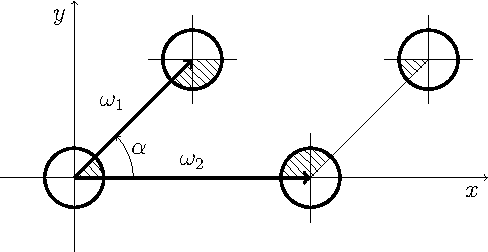
\includegraphics[width=7.5cm]{monoclin.pdf}
\caption{Моноклинная структура упаковки композиционной среды
\label{f:7:1}}}\hfil\hfil
\parbox[b]{7.5cm}{\centering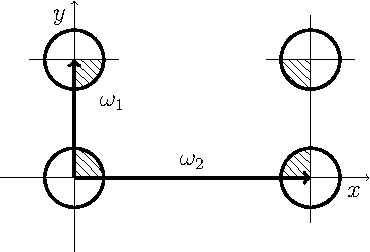
\includegraphics[width=5.8cm]{orthoromb.pdf}
\caption{Орторомбическая структура упаковки композиционной среды
\label{f:7:2}}}
\end{figure}

%\begin{figure}[h!]
%\centering
%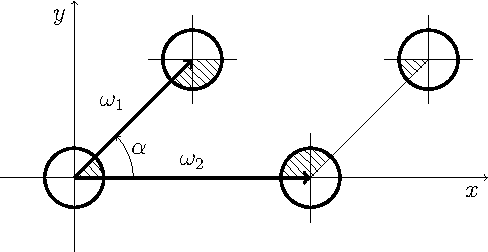
\includegraphics[width=8cm]{monoclin.pdf}
%\caption{Моноклинная структура упаковки композиционной среды}
%\label{f:7:1}
%\end{figure}

\textit{Орторомбическая структура} (рис.~\ref{f:7:2}), образованная цилиндрами с осями в вершинах прямоугольников. Эта структура соответствует ортотропной анизотропии.

%\begin{figure}[h!]
%\centering
%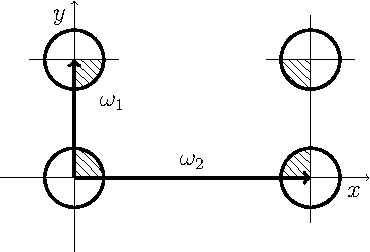
\includegraphics[width=6.5cm]{orthoromb.pdf}
%\caption{Орторомбическая структура упаковки композиционной среды}
%\label{f:7:2}
%\end{figure}

\textit{Тетрагональная структура} (рис.~\ref{f:7:3}), также соответствующая ортотропной анизотропии.

\begin{figure}[h!]
\centering\footnotesize
\parbox[b]{7.5cm}{\centering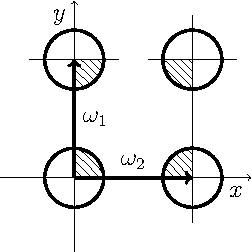
\includegraphics[width=4.5cm]{tetrahon.pdf}
\caption{Тетрагональная структура упаковки композиционной среды
\label{f:7:3}}}\hfil\hfil
\parbox[b]{7.5cm}{\centering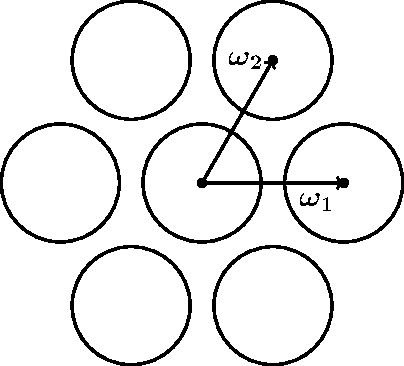
\includegraphics[width=4.5cm]{hexagonal-centroid-structure.pdf}
\caption{Гексагональная структура упаковки композиционной среды
\label{f:7:4}}}
\end{figure}

%\begin{figure}[h!]
%\centering
%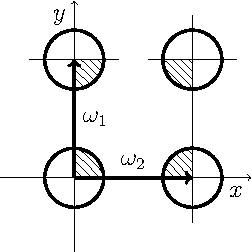
\includegraphics[width=4.5cm]{tetrahon.pdf}
%\caption{Тетрагональная структура упаковки композиционной среды}
%\label{f:7:3}
%\end{figure}

\textit{Гексагональная структура} (рис.~\ref{f:7:4}), обладающая наибольшей симметрией. Она соответствует трансверсально-изотропной анизотропии материала.

%\begin{figure}[h!]
%\centering
%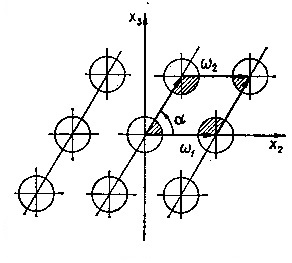
\includegraphics[width=8cm]{hexagon.jpg}
%\caption{Гексагональная структура упаковки композиционной среды}
%\label{f:7:4}
%\end{figure}

Важной характеристикой композита является объемное содержание волокна в матрице. Для разных структур упаковок можно вычислить предельное объемное содержание, при котором волокна в упаковке касаются друг друга. В работе~\cite{Vanin1985} приведены результаты
$$
\zeta_{max}=\frac{\pi}{2\sqrt{3}}\approx 0.91,
$$
$$
\zeta_{max}=\frac{\pi}{4}\approx 0.79
$$
соответственно для гексагональной и тетрагональной структур.

\section{Упругое состояние пористого материала с линейной регулярной структурой}

Рассмотрим цилиндрический образец однонаправленного пористого материала. Поры имеют форму одинаковых бесконечных круговых цилиндров радиуса $R$ (рис.~\ref{fig:cyl-4a}). Представительскую ячейку материала будем характеризовать расположением центров $\{O_j\}_{j=1}^N$ круговых сечений волокон плоскостью, перпендикулярной оси образца. Пусть $O_0$~--- центр представительской ячейки. Если ячейка объемно центрирована, то считаем, что $O_0$ совпадает с $O_1$, в противном случае $O_0$ не совпадает с $O_j$ $(j=\overline{1,N})$.

Введем цилиндрические системы координат $\left( {{\rho _j},{z_j},{\varphi _j}} \right)$ с началами в точках $O_j$, оси $O_jz_j$ которых совпадают с осями цилиндров.

Координаты в введенных системах координат связаны соотношениями

\begin{equation}
\left\{ {\begin{array}{*{20}{l}}
{{x_j} = {x_\alpha } + {x_{j\alpha }},}\\
{{y_j} = {y_\alpha } + {y_{j\alpha }},}\\
{{z_j} = {z_\alpha },}
\end{array}} \right.\qquad {\kern 1pt} j \ne \alpha ,\quad j,\alpha  = \overline {1,N},
\label{eq:7:25}
\end{equation}

\begin{equation}
\left\{ \begin{array}{l}
{x_j} = {\rho _j}\cos {\varphi _j},\\
{y_j} = {\rho _j}\sin {\varphi _j},
\end{array} \right.
\label{eq:7:26}
\end{equation}
где $\mathbf{O_jO_\alpha}=(x_{j\alpha},y_{j\alpha})=(\rho_{j\alpha},\varphi_{j\alpha})$.
 
\begin{figure}
\centering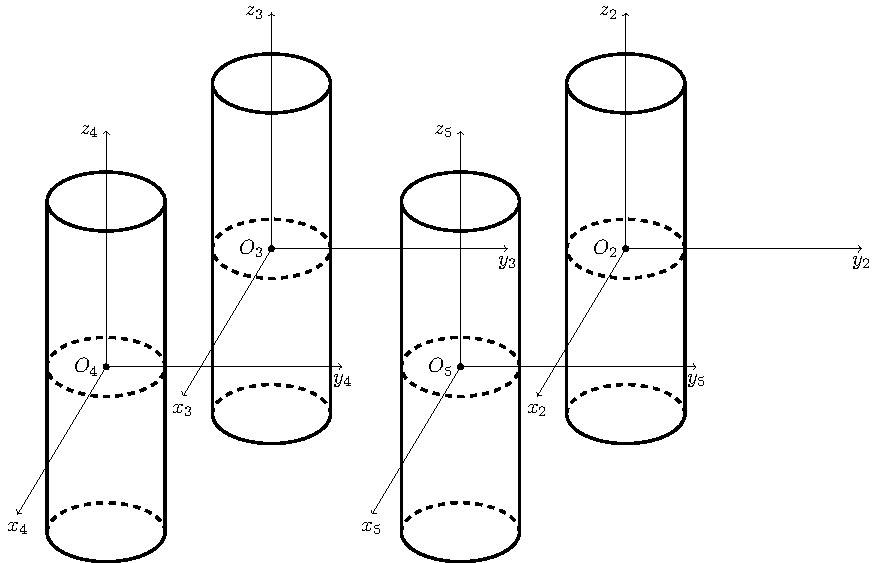
\includegraphics[width=12cm]{cylinders-4.pdf}
\caption{Схематическое представление задачи}
\label{fig:cyl-4a}
\end{figure}

Считаем, что цилиндрические полости свободны от нагрузки. Для определения НДС в рассматриваемом теле необходимо решить краевую задачу для уравнения Ламе

\begin{equation}
\Delta {\bf{U}} + \frac{1}{{1 - 2\sigma }}\nabla div{\bf{U}} = 0
\label{eq:7:27}
\end{equation}

\noindent с граничными условиями

\begin{equation}
{\bf{FU}}{|_{{\Gamma _j}}} = 0
\label{eq:7:18}
\end{equation}

\noindent и кусочно-постоянными напряжениями на цилиндрическом образце

\begin{equation}
{\left. {{\bf{FU}}} \right|_{{\Gamma _0}}} = \left\{ \begin{array}{l}
T,\;\;\;{\mkern 1mu} {\kern 1pt} |z| \le h/2\\
0,\;\;\;{\mkern 1mu} {\kern 1pt} |z| > h/2
\end{array} \right\}{{\bf{e}}_\rho },
\label{eq:7:19}
\end{equation}

\noindent где $\mathbf{U}$~--- вектор перемещений; $\mathbf{FU}$~--- отвечающий $\mathbf{U}$ вектор усилий на соответствующей граничной поверхности; границы цилиндров $\Gamma_j$ задаются уравнениями $\rho_j=R_j$ ($j=\overline{1,N}$).

Решение задачи будем искать в виде

\begin{equation}
\mathbf{U}^++\mathbf{U}^-,
\end{equation}

\noindent где

\begin{equation}
{\bf{U}}^+ = \sum\limits_{j = 1}^N {\sum\limits_{s = 1}^3 {\sum\limits_{m =  - \infty }^\infty  {\int\limits_{ - \infty }^\infty  {A_{s,m}^{(j)}} } } } (\lambda ){\bf{U}}_{s,\lambda ,m}^{ + (3)}\left( {{\rho _j},{z_j},{\varphi _j}} \right)d\lambda;
\end{equation}

\begin{equation}
{{\bf{U}}}^- = \sum\limits_{s = 1}^3 {\sum\limits_{m =  - \infty }^\infty  {\mathop \int \limits_{ - \infty }^\infty  } } A_{s,m}^{(0)}(\lambda ){\bf{U}}_{s,\lambda ,m}^{ - (3)}\left( {{\rho _1},{z_1},{\varphi _1}} \right)d\lambda;
\end{equation}

\noindent $A_{s,m}^{(j)}(\lambda )$~--- неизвестные функции;

\begin{equation}
\mathbf{U}_{s,\lambda,m}^{\pm(3)}(\rho,\varphi,z)=\lambda^{-1}\mathbf{D}_s u_{\lambda,m}^{\pm(3)}(\rho,\varphi,z);\quad s=1,3;
\label{eq:7:1}
\end{equation}

\begin{equation}
\mathbf{U}_{2,\lambda,m}^{\pm(3)}(\rho,\varphi,z)=\lambda^{-1}\mathbf{B}_2 u_{\lambda,m}^{\pm(3)}(\rho,\varphi,z),
\label{eq:7:2}
\end{equation}

\begin{equation}
\mathbf{B}_2=\left(x\frac{\partial}{\partial x}+y\frac{\partial}{\partial y}\right)\nabla-\chi\Big[\mathbf{e}_z\times[\nabla\times\mathbf{e}_z]\Big];
\end{equation}

\begin{equation*}
u_{\lambda,m}^{+(3)}(\rho,\varphi,z)=e^{i\lambda z+im\varphi}\tilde K_m(\lambda\rho),
\end{equation*}

\begin{equation*}
u_{\lambda,m}^{-(3)}(\rho,\varphi,z)=e^{i\lambda z+im\varphi}I_m(\lambda\rho),
\end{equation*}

\noindent где $\mathbf{D}_1=\nabla$, $\mathbf{D}_2=z\nabla-\chi\mathbf{e}_z$, $\mathbf{D}_3=i[\nabla\times\mathbf{e}_z]$ (здесь $i$~--- мнимая единица); $I_m(x)$~--- модифицированная функция Бесселя, $\tilde K_m(x)=(\mathrm{sign}\,x)^m K_m(|x|)$, $K_m(x)$~--- функция Макдональда; $\chi=3-4\sigma$, $u_{\lambda,m}^{\pm(3)}$~--- полный набор частных решений уравнения Лапласа в цилиндрических координатах.

В развернутой координатной форме базисные решения~\eqref{eq:7:1}, \eqref{eq:7:2} имеют вид:

\begin{equation}
\mathbf{U}_{1,\lambda,m}^{\pm(3)}(\rho,\varphi,z)=\mp u_{\lambda,m-1}^{\pm(3)}\mathbf{e}_{-1}\mp u_{\lambda,m+1}^{\pm(3)}\mathbf{e}_1+iu_{\lambda,m}^{\pm(3)}\mathbf{e}_0;
\label{eq:7:4}
\end{equation}

\begin{equation}
\mathbf{U}_{2,\lambda,m}^{\pm(3)}(\rho,\varphi,z)=\mp(D-\chi)\left[u_{\lambda,m-1}^{\pm(3)}\mathbf{e}_{-1}+
u_{\lambda,m+1}^{\pm(3)}\mathbf{e}_1\right]+iDu_{\lambda,m}^{\pm(3)}\mathbf{e}_0;
\label{eq:7:5}
\end{equation}

\begin{equation}
\mathbf{U}_{3,\lambda,m}^{\pm(3)}(\rho,\varphi,z)=\pm u_{\lambda,m-1}^{\pm(3)}\mathbf{e}_{-1}\mp u_{\lambda,m+1}^{\pm(3)}\mathbf{e}_1,
\label{eq:7:6}
\end{equation}

\noindent где $D=\rho\dfrac{\partial}{\partial\rho}$; $\mathbf{e}_{-1}=\dfrac{1}{2}(\mathbf{e}_\rho+i\mathbf{e}_\varphi)e^{i\varphi}$; $\mathbf{e}_1=\dfrac{1}{2}(\mathbf{e}_\rho-i\mathbf{e}_\varphi)e^{-i\varphi}$; $\mathbf{e}_0=\mathbf{e}_z$; $(\mathbf{e}_\rho,\mathbf{e}_\varphi,\mathbf{e}_z)$~--- орты цилиндрической системы координат.

Вектор напряжений на площадке с нормалью $\mathbf{n}$

\begin{equation}
\mathbf{FU}=2G\left[\frac{\sigma}{1-2\sigma}\mathbf{n}\,\mathrm{div}\mathbf{U}+\frac{\partial\mathbf{U}}{\partial\mathbf{n}}+\frac{1}{2}(\mathbf{n}\times\mathrm{rot}\mathbf{U})\right],
\label{eq:7:3}
\end{equation}

\noindent где $G$~--- модуль сдвига.

Применив к формулам~\eqref{eq:7:4}~--- \eqref{eq:7:6} оператор~\eqref{eq:7:3} на площадке с нормалью $\mathbf{n}=\mathbf{e}_\rho$, получим

\begin{equation}
\mathbf{FU}_{1,\lambda,m}^{\pm(3)}=\frac{2G}{\rho}\left\{\mp Du_{\lambda,m-1}^{\pm(3)}\mathbf{e}_{-1}\mp Du_{\lambda,m+1}^{\pm(3)}\mathbf{e}_1+iDu_{\lambda,m}^{\pm(3)}\mathbf{e}_0\right\};
\end{equation}

\begin{multline}
\mathbf{FU}_{2,\lambda,m}^{\pm(3)}= \\
= \frac{2G}{\rho}\left\{\mp\Big[(m-1)(m-1+2\sigma)+\lambda^2\rho^2+(2\sigma-3)D\Big]u_{\lambda,m-1}^{\pm(3)}\mathbf{e}_{-1}\mp\right.\\
\mp[(m+1)(m+1-2\sigma)+\lambda^2\rho^2+(2\sigma-3)D]u_{\lambda,m+1}^{\pm(3)}\mathbf{e}_1+\\
\left.+i[m^2+\lambda^2\rho^2(2\sigma-2)D]u_{\lambda,m}^{\pm(3)}\mathbf{e}_0\right\};
\end{multline}

\begin{multline}
\mathbf{FU}_{3,\lambda,m}^{\pm(3)}=\frac{G}{\rho}\left\{\pm(D+m-1)u_{\lambda,m-1}^{\pm(3)}\mathbf{e}_{-1}\mp\right.\\
\left.\mp(D-m-1)u_{\lambda,m+1}^{\pm(3)}\mathbf{e}_1-imu_{\lambda,m}^{\pm(3)}\mathbf{e}_0\right\}.
\end{multline}

Для удовлетворения граничных условий нам понадобятся теоремы сложения базисных решений уравнения Ламе для цилиндра:

\begin{equation}
{\bf{U}}_{s,\lambda ,m}^{ + (3)}\left( {{\rho _j},{z_j},{\varphi _j}} \right) = \sum\limits_{l =  - \infty }^\infty  {{{( - 1)}^l}} f_{\lambda ,m,j,\alpha }^{ + (33)l}{\bf{U}}_{s,\lambda ,l}^{ - (3)}\left( {{\rho _\alpha },{z_\alpha },{\varphi _\alpha }} \right);
\label{eq:7:7}
\end{equation}

\begin{multline}
{\bf{U}}_{2,\lambda ,m}^{ + (3)}\left( {{\rho _j},{z_j},{\varphi _j}} \right) = \sum\limits_{l =  - \infty }^\infty  {{{( - 1)}^l}} \left[ {f_{\lambda ,m,j,\alpha }^{ + (33)l}{\bf{U}}_{2,\lambda ,l}^{ - (3)}\left( {{\rho _\alpha },{z_\alpha },{\varphi _\alpha }} \right) + } \right.\\
\left. { + \tilde f_{\lambda ,m,j,\alpha }^{ + (33)l}{\bf{U}}_{1,\lambda ,l}^{ - (3)}\left( {{\rho _\alpha },{z_\alpha },{\varphi _\alpha }} \right)} \right];
\label{eq:7:8}
\end{multline}

$$
f_{\lambda ,m,j,\alpha }^{ + (33)l} = u_{\lambda ,m - l}^{ + (3)}\left( {{\rho _{j\alpha }},{z_{j\alpha }},{\varphi _{j\alpha }}} \right),
$$
$$
\tilde f_{\lambda ,m,j,\alpha }^{ + (33)l} = {\rho _{j\alpha }}\frac{\partial }{{\partial {\rho _{j\alpha }}}}u_{\lambda ,m - l}^{ + (3)}\left( {{\rho _{j\alpha }},{z_{j\alpha }},{\varphi _{j\alpha }}} \right);
$$

\begin{equation}
{\bf{U}}_{s,\lambda ,m}^{ - (3)}\left( {{\rho _0},{z_0},{\varphi _0}} \right) = \sum\limits_{l =  - \infty }^\infty  {f_{\lambda ,m,j}^{ - (33)l}{\bf{U}}_{s,\lambda ,l}^{ - (3)}\left( {{\rho _j},{z_j},{\varphi _j}} \right)};
\label{eq:7:9}
\end{equation}

\begin{multline}
{\bf{U}}_{2,\lambda ,m}^{ - (3)}\left( {{\rho _0},{z_0},{\varphi _0}} \right) = \sum\limits_{l =  - \infty }^\infty  {\left[ {f_{\lambda ,m,j}^{ - (33)l}{\bf{U}}_{2,\lambda ,l}^{ - (3)}\left( {{\rho _j},{z_j},{\varphi _j}} \right) + } \right.} \\
\left. { + \tilde f_{\lambda ,m,j}^{ - (33)l}{\bf{U}}_{1,\lambda ,l}^{ - (3)}\left( {{\rho _j},{z_j},{\varphi _j}} \right)} \right];
\label{eq:7:10}
\end{multline}

$$
f_{\lambda ,m,j}^{ - (33)l} = u_{\lambda ,m - l}^{ - (3)}\left( {{\rho _{0j}},{z_{0j}},{\varphi _{0j}}} \right),
$$
$$
\tilde f_{\lambda ,m,j}^{ - (33)l} = {\rho _{0j}}\frac{\partial }{{\partial {\rho _{0j}}}}u_{\lambda ,m - l}^{ - (3)}\left( {{\rho _{0j}},{z_{0j}},{\varphi _{0j}}} \right);
$$

\begin{equation}
{\bf{U}}_{s,\lambda ,m}^{ + (3)}\left( {{\rho _j},{z_j},{\varphi _j}} \right) = \sum\limits_{l =  - \infty }^\infty  {f_{\lambda ,m,j}^{ - (33)l}{\bf{U}}_{s,\lambda ,l}^{ + (3)}\left( {{\rho _0},{z_0},{\varphi _0}} \right)};
\label{eq:7:11}
\end{equation}

\begin{multline}
{\bf{U}}_{2,\lambda ,m}^{ + (3)}\left( {{\rho _j},{z_j},{\varphi _j}} \right) = \sum\limits_{l =  - \infty }^\infty  {\left[ {f_{\lambda ,m,j}^{ - (33)l}{\bf{U}}_{2,\lambda ,l}^{ - (3)}\left( {{\rho _0},{z_0},{\varphi _0}} \right) + } \right.} \\
\left. { + \tilde f_{\lambda ,m,j}^{ - (33)l}{\bf{U}}_{1,\lambda ,l}^{ + (3)}\left( {{\rho _0},{z_0},{\varphi _0}} \right)} \right];
\label{eq:7:12}
\end{multline}

$$
f_{\lambda ,m,j}^{ - (33)l} = u_{\lambda ,m - l}^{ - (3)}\left( {{\rho _{0j}},{z_{0j}},{\varphi _{0j}}} \right),
$$
$$
\tilde f_{\lambda ,m,j}^{ - (33)l} = {\rho _{0j}}\frac{\partial }{{\partial {\rho _{0j}}}}u_{\lambda ,m - l}^{ - (3)}\left( {{\rho _{0j}},{z_{0j}},{\varphi _{0j}}} \right).
$$

Запишем общее решение в системе координат с началами $O_0$ и $O_\alpha$ с помощью теорем сложения~\eqref{eq:7:7}~--- \eqref{eq:7:12}. В случае, если ячейка не является объемно центрированной,

\begin{multline}
{\bf{U}} = \sum\limits_{s = 1}^3 {\sum\limits_{m =  - \infty }^\infty  {\int\limits_{ - \infty }^\infty\bigg\{  } } A_{s,m}^{(0)}(\lambda ){\bf{U}}_{s,\lambda ,m}^{ - (3)}({\rho _0},{z_0},{\varphi _0}) + \\
+ {\bf{U}}_{s,\lambda ,m}^{ + (3)}({\rho _0},{z_0},{\varphi _0})\sum\limits_{\alpha  = 1}^N {\sum\limits_{t = 1}^3 {\sum\limits_{l =  - \infty }^\infty  {A_{t,l}^{(\alpha )}} } } (\lambda )\bigg[{\delta _{st}} + \\
+ {\delta _{s1}}{\delta _{t2}}{\rho _{0\alpha }}\frac{\partial }{{\partial {\rho _{0\alpha }}}}\bigg]u_{\lambda ,l - m}^{ - (3)}({\rho _{0\alpha }},0,{\varphi _{0\alpha }})\bigg\} d\lambda;
\label{eq:7:13}
\end{multline}

\begin{multline}
{\bf{U}} = \sum\limits_{s = 1}^3 {\sum\limits_{m =  - \infty }^\infty  {\int\limits_{ - \infty }^\infty  \bigg\{  } } A_{s,m}^{(\alpha )}(\lambda ){\bf{U}}_{s,\lambda ,m}^{ + (3)}({\rho _\alpha },{z_\alpha },{\varphi _\alpha }) + \\
+ {\bf{U}}_{s,\lambda ,m}^{ - (3)}({\rho _\alpha },{z_\alpha },{\varphi _\alpha })\sum\limits_{t = 1}^3 {\sum\limits_{l =  - \infty }^\infty  {A_{t,l}^{(0)}} } (\lambda )\bigg[{\delta _{st}} + \\
+ {\delta _{s1}}{\delta _{t2}}{\rho _{0\alpha }}\frac{\partial }{{\partial {\rho _{0\alpha }}}}\bigg]u_{\lambda ,l - m}^{ - (3)}({\rho _{0\alpha }},0,{\varphi _{0\alpha }}) + \\
+ \sum\limits_{j \ne \alpha } {{\bf{U}}_{s,\lambda ,m}^{ - (3)}} ({\rho _\alpha },{z_\alpha },{\varphi _\alpha })\sum\limits_{t = 1}^3 {\sum\limits_{l =  - \infty }^\infty  {A_{t,l}^{(j)}} } (\lambda ){( - 1)^m}\bigg[{\delta _{st}} + \\
+ {\delta _{s1}}{\delta _{t2}}{\rho _{j\alpha }}\frac{\partial }{{\partial {\rho _{j\alpha }}}}\bigg]u_{\lambda ,l - m}^{ + (3)}({\rho _{j\alpha }},0,{\varphi _{j\alpha }})\bigg\} d\lambda.
\label{eq:7:14}
\end{multline}

В случае объемно центрированной ячейки вектор перемещения имеет вид:

\begin{multline}
{\bf{U}} = \sum\limits_{s = 1}^3 {\sum\limits_{m =  - \infty }^\infty  {\int\limits_{ - \infty }^\infty  \bigg\{  } } A_{s,m}^{(0)}(\lambda ){\bf{U}}_{s,\lambda ,m}^{ - (3)}({\rho _1},{z_1},{\varphi _1}) + \\
+ A_{s,m}^{(1)}(\lambda ){\bf{U}}_{s,\lambda ,m}^{ + (3)}({\rho _1},{z_1},{\varphi _1}) + {\bf{U}}_{s,\lambda ,m}^{ + (3)}({\rho _1},{z_1},{\varphi _1})\sum\limits_{\alpha  = 2}^N {\sum\limits_{t = 1}^3 {\sum\limits_{l =  - \infty }^\infty  {A_{t,l}^{(\alpha )}} } } (\lambda )\bigg[{\delta _{st}} + \\
+ {\delta _{s1}}{\delta _{t2}}{\rho _{1\alpha }}\frac{\partial }{{\partial {\rho _{1\alpha }}}}\bigg]u_{\lambda ,l - m}^{ - (3)}({\rho _{1\alpha }},0,{\varphi _{1\alpha }})\bigg\} d\lambda;
\label{eq:7:15}
\end{multline}

\begin{multline}
{\bf{U}} = \sum\limits_{s = 1}^3 {\sum\limits_{m =  - \infty }^\infty  {\int\limits_{ - \infty }^\infty  \bigg\{  } } A_{s,m}^{(0)}(\lambda ){\bf{U}}_{s,\lambda ,m}^{ - (3)}({\rho _1},{z_1},{\varphi _1}) + \\
+ A_{s,m}^{(1)}(\lambda ){\bf{U}}_{s,\lambda ,m}^{ + (3)}({\rho _1},{z_1},{\varphi _1}) + \\
+ {\bf{U}}_{s,\lambda ,m}^{ - (3)}({\rho _1},{z_1},{\varphi _1})\sum\limits_{\alpha  = 2}^N {\sum\limits_{t = 1}^3 {\sum\limits_{l =  - \infty }^\infty  {A_{t,l}^{(\alpha )}} } } (\lambda ){( - 1)^l}\bigg[{\delta _{st}} + \\
+ {\delta _{s1}}{\delta _{t2}}{\rho _{1\alpha }}\frac{\partial }{{\partial {\rho _{1\alpha }}}}\bigg]u_{\lambda ,l - m}^{ + (3)}({\rho _{1\alpha }},0,{\varphi _{1\alpha }})\bigg\} d\lambda;
\label{eq:7:16}
\end{multline}

\begin{multline}
{\bf{U}} = \sum\limits_{s = 1}^3 {\sum\limits_{m =  - \infty }^\infty  {\int\limits_{ - \infty }^\infty  \bigg\{  } } A_{s,m}^{(\alpha )}(\lambda ){\bf{U}}_{s,\lambda ,m}^{ + (3)}({\rho _\alpha },{z_\alpha },{\varphi _\alpha }) + \\
+ {\bf{U}}_{s,\lambda ,m}^{ - (3)}({\rho _\alpha },{z_\alpha },{\varphi _\alpha })\sum\limits_{t = 1}^3 {\sum\limits_{l =  - \infty }^\infty  {A_{t,l}^{(0)}} } (\lambda )\bigg[{\delta _{st}} + \\
+ {\delta _{s1}}{\delta _{t2}}{\rho _{0\alpha }}\frac{\partial }{{\partial {\rho _{0\alpha }}}}\bigg]u_{\lambda ,l - m}^{ - (3)}({\rho _{0\alpha }},0,{\varphi _{0\alpha }}) + \\
+ \sum\limits_{j \ne \alpha } {{\bf{U}}_{s,\lambda ,m}^{ - (3)}} ({\rho _\alpha },{z_\alpha },{\varphi _\alpha })\sum\limits_{t = 1}^3 {\sum\limits_{l =  - \infty }^\infty  {A_{t,l}^{(j)}} } (\lambda ){( - 1)^m}\bigg[{\delta _{st}} + \\
+ {\delta _{s1}}{\delta _{t2}}{\rho _{j\alpha }}\frac{\partial }{{\partial {\rho _{j\alpha }}}}\bigg]u_{\lambda ,l - m}^{ + (3)}({\rho _{j\alpha }},0,{\varphi _{j\alpha }})\bigg\} d\lambda ,\qquad {\kern 1pt} \alpha  \ne 1.
\label{eq:7:17}
\end{multline}

Переходя в формулах~\eqref{eq:7:13}~--- \eqref{eq:7:17} к напряжениям на поверхности $\Gamma_j$, согласно соотношениям~\eqref{eq:7:18}, \eqref{eq:7:19}, относительно неизвестных функций $A_{s,m}^{(j)}(\lambda)$ получаем бесконечную систему линейных алгебраических уравнений\sloppy

\begin{multline}
\sum\limits_{s = 1}^3 \bigg\{  A_{s,m}^{(0)}(\lambda ){\bf{G}}_{s,\lambda ,m}^{ - (3)}({R_0},G,\sigma ) + {\bf{G}}_{s,\lambda ,m}^{ + (3)}({R_0},G,\sigma ) \times \\
\times \sum\limits_{\alpha  = 1}^N {\sum\limits_{t = 1}^3 {\sum\limits_{l =  - \infty }^\infty  {A_{t,l}^{(\alpha )}} } } (\lambda )\bigg[{\delta _{st}} + {\delta _{s1}}{\delta _{t2}}{\rho _{0\alpha }}\frac{\partial }{{\partial {\rho _{0\alpha }}}}\bigg]u_{\lambda ,l - m}^{ - (3)}({\rho _{0\alpha }},0,{\varphi _{0\alpha }})\bigg\}  = \\
= \frac{T}{\pi }\frac{{\sin \lambda h}}{\lambda }{\delta _{m0}}(1,1,0),
\label{eq:7:20}
\end{multline}

\begin{multline}
\sum\limits_{s = 1}^3 \bigg\{  A_{s,m}^{(\alpha )}(\lambda ){\bf{G}}_{s,\lambda ,m}^{ + (3)}(R,G,\sigma ) + {\bf{G}}_{s,\lambda ,m}^{ - (3)}(R,G,\sigma ) \times \\
\times \sum\limits_{t = 1}^3 {\sum\limits_{l =  - \infty }^\infty  {A_{t,l}^{(0)}} } (\lambda )\bigg[{\delta _{st}} + {\delta _{s1}}{\delta _{t2}}{\rho _{0\alpha }}\frac{\partial }{{\partial {\rho _{0\alpha }}}}\bigg]u_{\lambda ,l - m}^{ - (3)}({\rho _{0\alpha }},0,{\varphi _{0\alpha }}) + \\
+ \sum\limits_{j \ne \alpha } {{\bf{G}}_{s,\lambda ,m}^{ - (3)}} (R,G,\sigma )\sum\limits_{t = 1}^3 {\sum\limits_{l =  - \infty }^\infty  {A_{t,l}^{(j)}} } (\lambda ){( - 1)^m}\bigg[{\delta _{st}} + {\delta _{s1}}{\delta _{t2}}{\rho _{j\alpha }}\frac{\partial }{{\partial {\rho _{j\alpha }}}}\bigg] \times \\
\times u_{\lambda ,l - m}^{ + (3)}({\rho _{j\alpha }},0,{\varphi _{j\alpha }})\bigg\}  = 0.
\label{eq:7:21}
\end{multline}

Система записана в случае отсутствия объемного центрирования. Для объем\-но-цент\-ри\-ро\-ван\-ной ячейки разрешающая система имеет вид:

\begin{multline}
\sum\limits_{s = 1}^3 \bigg\{  A_{s,m}^{(0)}(\lambda ){\bf{G}}_{s,\lambda ,m}^{ - (3)}({R_0},G,\sigma ) + A_{s,m}^{(1)}(\lambda ){\bf{G}}_{s,\lambda ,m}^{ + (3)}({R_0},G,\sigma ) + \\
+ {\bf{G}}_{s,\lambda ,m}^{ + (3)}({R_0},G,\sigma )\sum\limits_{\alpha  = 2}^N {\sum\limits_{t = 1}^3 {\sum\limits_{l =  - \infty }^\infty  {A_{t,l}^{(\alpha )}} } } (\lambda )\bigg[{\delta _{st}} + \\
+ {\delta _{s1}}{\delta _{t2}}{\rho _{0\alpha }}\frac{\partial }{{\partial {\rho _{0\alpha }}}}\bigg]u_{\lambda ,l - m}^{ - (3)}({\rho _{0\alpha }},0,{\varphi _{0\alpha }})\bigg\}  = \frac{T}{\pi }\frac{{\sin \lambda h}}{\lambda }{\delta _{m0}}(1,1,0);
\label{eq:7:22}
\end{multline}

\begin{multline}
\sum\limits_{s = 1}^3 \bigg\{  A_{s,m}^{(\alpha )}(\lambda ){\bf{G}}_{s,\lambda ,m}^{ + (3)}(R,G,\sigma ) + {\bf{G}}_{s,\lambda ,m}^{ - (3)}(R,G,\sigma ) \times \\
\times \sum\limits_{t = 1}^3 {\sum\limits_{l =  - \infty }^\infty  {A_{t,l}^{(0)}} } (\lambda )\bigg[{\delta _{st}} + {\delta _{s1}}{\delta _{t2}}{\rho _{0\alpha }}\frac{\partial }{{\partial {\rho _{0\alpha }}}}\bigg]u_{\lambda ,l - m}^{ - (3)}({\rho _{0\alpha }},0,{\varphi _{0\alpha }}) + \\
+ \sum\limits_{j \ne \alpha } {{\bf{G}}_{s,\lambda ,m}^{ - (3)}} (R,G,\sigma )\sum\limits_{t = 1}^3 {\sum\limits_{l =  - \infty }^\infty  {A_{t,l}^{(j)}} } (\lambda ){( - 1)^m}\bigg[{\delta _{st}} + {\delta _{s1}}{\delta _{t2}}{\rho _{j\alpha }}\frac{\partial }{{\partial {\rho _{j\alpha }}}}\bigg] \times \\
\times u_{\lambda ,l - m}^{ + (3)}({\rho _{j\alpha }},0,{\varphi _{j\alpha }})\bigg\}  = 0,\qquad {\kern 1pt} \alpha  \ne 1;
\label{eq:7:23}
\end{multline}

\begin{multline}
\sum\limits_{s = 1}^3 \bigg\{  A_{s,m}^{(0)}(\lambda ){\bf{G}}_{s,\lambda ,m}^{ - (3)}(R,G,\sigma ) + A_{s,m}^{(1)}(\lambda ){\bf{G}}_{s,\lambda ,m}^{ + (3)}(R,G,\sigma ) + \\
+ \mathop \sum \limits_{j = 2}^N {\bf{G}}_{s,\lambda ,m}^{ - (3)}(R,G,\sigma )\sum\limits_{t = 1}^3 {\sum\limits_{l =  - \infty }^\infty  {A_{t,l}^{(j)}} } (\lambda ){( - 1)^m}\bigg[{\delta _{st}} + {\delta _{s1}}{\delta _{t2}}{\rho _{j1}}\frac{\partial }{{\partial {\rho _{j1}}}}\bigg] \times \\
\times u_{\lambda ,l - m}^{ + (3)}({\rho _{j1}},0,{\varphi _{j1}})\bigg\}  = 0;
\label{eq:7:24}
\end{multline}

\begin{equation}
G_{1,\lambda ,m}^{ \pm ( - 1)}(R) =  \mp \frac{{2G}}{R}D\tilde u_{\lambda ,m - 1}^{ \pm (3)}(R),\, G_{1,\lambda ,m}^{ \pm (1)}(R) =  \pm \frac{{2G}}{R}D\tilde u_{\lambda ,m + 1}^{ \pm (3)}(R);
\label{eq:7:35}
\end{equation}
\begin{equation}
G_{1,\lambda ,m}^{ \pm (0)}(R) = \frac{{2G}}{R}iD\tilde u_{\lambda ,m}^{ \pm (3)}(R);
\label{eq:7:36}
\end{equation}
\begin{multline}
G_{2,\lambda ,m}^{ \pm ( - 1)}(R) = \mp \frac{{2G}}{R}\bigg[(m - 1)(m - 1 + 2\sigma ) + \\
+ {\lambda ^2}{R^2} + (2\sigma  - 3)D\bigg]\tilde u_{\lambda ,m - 1}^{ \pm (3)}(R);
\label{eq:7:37}
\end{multline}
\begin{multline}
G_{2,\lambda ,m}^{ \pm (1)}(R) = \mp \frac{{2G}}{R}\bigg[ (m + 1)(m + 1 - 2\sigma ) + \\
+ {\lambda ^2}{R^2} + (2\sigma  - 3)D \bigg]\tilde u_{\lambda ,m + 1}^{ \pm (3)}(R);
\label{eq:7:38}
\end{multline}
\begin{equation}
G_{2,\lambda ,m}^{ \pm (0)}(R) = \frac{{2G}}{R}i\left[ {{m^2} + {\lambda ^2}{R^2} + (2\sigma  - 2)D} \right]\tilde u_{\lambda ,m}^{ \pm (3)}(R);
\label{eq:7:39}
\end{equation}
\begin{equation}
G_{3,\lambda ,m}^{ \pm ( - 1)}(R) =  \pm \frac{G}{R}\left( {D + m - 1} \right)\tilde u_{\lambda ,m - 1}^{ \pm (3)}(R);
\label{eq:7:40}
\end{equation}
\begin{equation}
G_{3,\lambda ,m}^{ \pm (1)}(R) =  \mp \frac{G}{R}\left( {D - m - 1} \right)\tilde u_{\lambda ,m + 1}^{ \pm (3)}(R);
\label{eq:7:41}
\end{equation}
\begin{equation}
G_{3,\lambda ,m}^{ \pm (0)}(R) =  - \frac{G}{R}im\tilde u_{\lambda ,m}^{ \pm (3)}(R);
\label{eq:7:41a}
\end{equation}
\begin{equation}
\tilde u_{\lambda ,m}^{ \pm (3)}(R) = \left\{ \begin{array}{l}
{{\tilde K}_m}\left( {\lambda R} \right)\\
{I_m}\left( {\lambda R} \right)
\end{array} \right\}.
\label{eq:7:42}
\end{equation}

\section{Анализ разрешающей системы}

\begin{theorem}
При любом $\lambda\neq 0$ оператор системы~\eqref{eq:7:20}, \eqref{eq:7:21} является фредгольмовым в гильбертовом пространстве $l_2$ при выполнении условий $R_j+R_\alpha<\rho_{j\alpha}$ ($j\neq\alpha$; $j,\alpha=1\div N$), $\rho_{0\alpha}+R_\alpha<R_0$ ($\alpha=1\div N$). 
\end{theorem}
\begin{proof}
Путем переобозначения неизвестных функций
\begin{equation}
A_{s,m}^{(j)}(\lambda)=\frac{\tilde A_{s,m}^{(j)}(\lambda)}{K_m(|\lambda|R_j)},\quad(j=1\div N),\quad A_{s,m}^{(0)}(\lambda)=\frac{\tilde A_{s,m}^{(0)}(\lambda)}{I_m(\lambda R_0)}
\end{equation}
и решения системы относительно $\tilde A_{s,m}^{(j)}(\lambda)$ можно представить систему~\eqref{eq:7:20}, \eqref{eq:7:21} в виде
\begin{multline}
\tilde A_{s,m}^{(\alpha)}(\lambda)+\sum\limits_{j\neq\alpha}\sum\limits_{p=1}^3\sum\limits_{l=-\infty}^\infty T_{1,\alpha,s,m}^{j,p,l}\tilde A_{p,l}^{(j)}(\lambda)+ \\
+ \sum\limits_{p=1}^3\sum\limits_{l=-\infty}^\infty T_{2,\alpha,s,m}^{p,l}\tilde A_{p,l}^{(0)}(\lambda)=0,
\label{eq:27}
\end{multline}
\begin{equation}
\tilde A_{s,m}^{(0)}(\lambda)+\sum\limits_{j=1}^N\sum\limits_{p=1}^3\sum\limits_{l=-\infty}^\infty T_{3,s,m}^{j,p,l}\tilde A_{p,l}^{(j)}(\lambda)=F_{s,m}(\lambda).
\label{eq:28}
\end{equation}
Опустим явную запись матричных коэффициентов. Заметим, что модули матричных коэффициентов $\left|T_{1,\alpha,s,m}^{j,p,l}\right|$, $\left|T_{2,\alpha,s,m}^{p,l}\right|$, $\left|T_{3,s,m}^{j,p,l}\right|$ оцениваются сверху конечными линейными комбинациями выражений вида~\eqref{eq:24}~--- \eqref{eq:26} соответственно:
\begin{equation}
\bigg|\frac{I_m(\lambda R_\alpha)}{K_l(|\lambda|R_j)}K_{m-l}(|\lambda|\rho_{j\alpha})\bigg|;
\label{eq:24}
\end{equation}
\begin{equation}
\bigg|\frac{I_m(\lambda R_\alpha)}{I_l(\lambda R_0)}I_{m-l}(|\lambda|\rho_{0\alpha})\bigg|;
\label{eq:25}
\end{equation}
\begin{equation}
\bigg|\frac{K_m(|\lambda|R_0)}{K_l(|\lambda|R_j)}I_{m-l}(\lambda\rho_{j0})\bigg|.
\label{eq:26}
\end{equation}
При этом были использованы оценки определителей разрешающих систем первой краевой задачи теории упругости для внутренности и внешности цилиндра, полученные в работе~\cite{Nikolaev1998}.

Для доказательства теоремы достаточно показать, выполнение следующих условий для матричных коэффициентов системы~\eqref{eq:27}, \eqref{eq:28}:
\begin{equation}
\sum\limits_{m=-\infty}^\infty\sum\limits_{l=-\infty}^\infty\bigg|T_{1,\alpha,s,m}^{j,p,l}\bigg|^2<\infty,
\end{equation}
\begin{equation}
\sum\limits_{m=-\infty}^\infty\sum\limits_{l=-\infty}^\infty\bigg|T_{2,\alpha,s,m}^{p,l}\bigg|^2<\infty,
\end{equation}
\begin{equation}
\sum\limits_{m=-\infty}^\infty\sum\limits_{l=-\infty}^\infty\bigg|T_{3,s,m}^{j,p,l}\bigg|^2<\infty.
\end{equation}
\par Рассмотрим теорему сложения гармонических функций~\cite{Nikolaev2011}:
\begin{multline}
u_{\lambda,m}^{+(3)}(\rho_j,\varphi_j,z_j)=\\
=\sum\limits_{l=-\infty}^\infty(-1)^l u_{\lambda,m-l}^{+(3)}(\rho_{j\alpha},\varphi_{j\alpha},z_{j\alpha}) u_{\lambda,l}^{-(3)}(\rho_\alpha,\varphi_\alpha,z_\alpha).
\end{multline}
Это разложение можно интепретировать как представление функции $u_{\lambda,m}^{+(3)}(\rho_j,\varphi_j,z_j)$ рядом Фурье по переменной $\varphi_\alpha\in[0,2\pi]$. Тогда для этого разложения справедливо равенство Парсеваля{\sloppy\par}
\begin{equation}
\sum\limits_{l=-\infty}^\infty\bigg|K_{m-l}(|\lambda|\rho_{j\alpha})\bigg|^2\bigg|I_l(\lambda\rho_\alpha)\bigg|^2=\frac{1}{2\pi}\int\limits_0^{2\pi}\bigg|K_m(|\lambda|\rho_j)\bigg|^2d\varphi_\alpha.
\label{eq:32}
\end{equation}
В силу оценок~\eqref{eq:24}~--- \eqref{eq:26} для доказательства теоремы достаточно показать сходимость рядов
\begin{equation}
\sum\limits_{m=-\infty}^\infty\sum\limits_{l=-\infty}^\infty\bigg|\frac{I_m(\lambda R_\alpha)}{K_l(|\lambda|R_j)}K_{m-l}(|\lambda|\rho_{j\alpha})\bigg|^2,
\label{eq:29}
\end{equation}
\begin{equation}
\sum\limits_{m=-\infty}^\infty\sum\limits_{l=-\infty}^\infty\bigg|\frac{I_m(\lambda R_\alpha)}{I_l(\lambda R_0)}I_{m-l}(|\lambda|\rho_{0\alpha})\bigg|^2,
\label{eq:30}
\end{equation}
\begin{equation}
\sum\limits_{m=-\infty}^\infty\sum\limits_{l=-\infty}^\infty\bigg|\frac{K_m(|\lambda|R_0)}{K_l(|\lambda|R_j)}I_{m-l}(\lambda\rho_{j0})\bigg|^2.
\label{eq:31}
\end{equation}
\par В работе~\cite{Nikolaev1998} доказана оценка
\begin{equation}
I_m(z)K_m(z)>\frac{c}{m^2+1}(1+2z)^{-1},\quad m\ge 0,\quad z>0,
\label{eq:37}
\end{equation}
где $c>0$~--- некоторая постоянная. Тогда ряд~\eqref{eq:29} можно мажорировать рядом
\begin{equation*}
\sum\limits_{m=-\infty}^\infty\sum\limits_{l=-\infty}^\infty\bigg|I_l(\lambda R_\alpha)I_m(\lambda R_j)K_{m-l}(|\lambda|\rho_{j\alpha})\bigg|^2.
\end{equation*}
Подставим в тождество~\eqref{eq:32} $\rho_\alpha=R_\alpha$, после чего домножим обе его части на $|I_m(\lambda R_j)|^2$ и просуммируем по $m$ от $-\infty$ до $\infty$. В результате получим
\begin{multline}
\sum\limits_{m=-\infty}^\infty\sum\limits_{l=-\infty}^\infty\bigg|I_l(\lambda R_\alpha)I_m(\lambda R_j)K_{m-l}(|\lambda|\rho_{j\alpha})\bigg|^2=\\
=\frac{1}{2\pi}\int\limits_0^{2\pi}\sum\limits_{m=0}^\infty\bigg|I_m(\lambda R_j)\bigg|^2\bigg|K_m(|\lambda|\rho_j)\bigg|_{|_{\rho_\alpha=R_\alpha}}^2d\varphi_\alpha.
\label{eq:33}
\end{multline}
Из асимптотических формул при $m\rightarrow\infty$~\cite{Lebedev}
\begin{equation}
I_m(z)=\bigg(\frac{z}{2}\bigg)^m\frac{1}{m!}\bigg[1+O(m^{-1})\bigg],
\label{eq:35}
\end{equation}
\begin{equation}
K_m(z)=\frac{2^{m-1}(m-1)!}{z^m}\bigg[1+O(m^{-1})\bigg]
\label{eq:36}
\end{equation}
следует, что ряд в левой части~\eqref{eq:33} сходится при условии $\rho_j>R_j$. Определим минимальное значение $\rho_j^{min}$ при произвольных значениях угла $\varphi_\alpha$. Из соотношений между цилиндрическими координатами в системах с началами $O_j$ и $O_\alpha$ следует, что при $\rho_\alpha=R_\alpha$
\begin{equation*}
\rho_j=\sqrt{\rho_{j\alpha}^2+R_\alpha^2+2\rho_{j\alpha}R_\alpha\cos{(\varphi_\alpha-\varphi_{j\alpha})}}
\end{equation*}
и минимальное значение $\rho_j$ достигается при условии $\varphi_\alpha-\varphi_{j\alpha}=\pi$ и равняется $\rho_j^{min}=\rho_{j\alpha}-R_\alpha$ ($\rho_{j\alpha}>R_\alpha$~--- естественное геометрическое условие в постановке задачи).

Таким образом, условие сходимости ряда будет удовлетворено, если $\rho_j^{min}>R_j$. Оно означает, что $R_j+R_\alpha<\rho_{j\alpha}$.{\sloppy\par}

Аналогично можно записать такое равенство:
\begin{multline}
\sum\limits_{m=-\infty}^\infty\sum\limits_{l=-\infty}^\infty\bigg|K_m(|\lambda| R_0)I_l(\lambda R_\alpha)I_{m-l}(\lambda\rho_{0\alpha})\bigg|^2=\\
=\frac{1}{2\pi}\int\limits_0^{2\pi}\sum\limits_{m=0}^\infty\bigg|K_m(|\lambda|R_0)\bigg|^2\bigg|I_m(\lambda\rho_0)\bigg|_{|_{\rho_\alpha=R_\alpha}}^2d\varphi_\alpha.
\label{eq:34}
\end{multline}
На основании асимптотик~\eqref{eq:35}, \eqref{eq:36} ряд в формуле~\eqref{eq:34} сходится при условии $\rho_0<R_0$. На поверхности $\rho_\alpha=R_\alpha$ справедливо $\rho_0^{max}=\rho_{0\alpha}+R_\alpha$. Поэтому условием сходимости ряда~\eqref{eq:34} является неравенство $\rho_0^{max}<R_0$ или $\rho_{0\alpha}+R_\alpha<R_0$.

В силу оценки~\eqref{eq:37} сходимость ряда~\eqref{eq:31} при условии $\rho_{0j}+R_j<R_0$ следует из сходимости ряда~\eqref{eq:34}.
\end{proof}


\section{Анализ напряженного состояния пористого материала}

Численное решение разрешающих систем~\eqref{eq:7:20}~--- \eqref{eq:7:24} позволяет найти распределение напряжений в пористом материале при любой структуре упаковки. Далее будут рассмотрены следующие варианты упаковки волокон: тетрагональная и гексагональная и их центрированные модификации.

Рассмотрим геометрическую конфигурацию, представленную на рис.~\ref{f:7:6}.

\begin{figure}[h!]
\centering
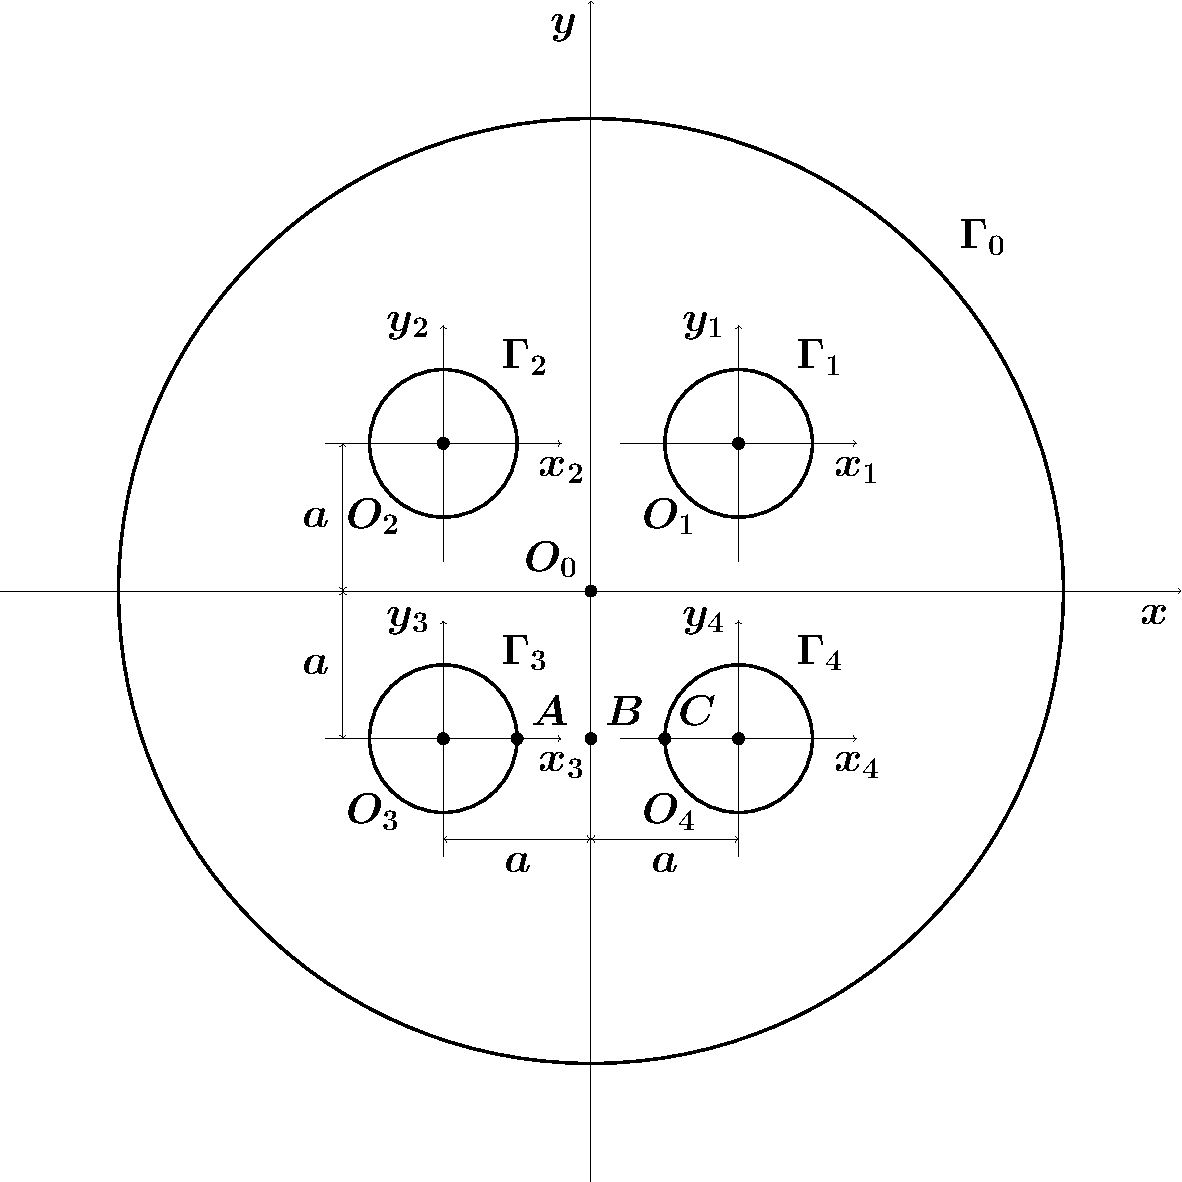
\includegraphics[width=12.2cm]{fig_7-6.pdf}
\caption{\centering Цилиндрический образец пористого материала с тетрагональной структурой упаковки}
\label{f:7:6}
\end{figure}

Коэффициент Пуассона материала $\sigma=0.38$, что соответствует материалу матрицы из эпоксидных смол. Толщина кольца, по которому прикладывается постоянная внешняя нагрузка $T$, $h=0.5R_0$; также считаем, что $R=1$, $R_0=10R$.

Несобственные интегралы, фигурирующие в формулах для определения напряжений, вычисляются по квадратурным формулам Гаусса~--- Лагерра с количеством узлов $n=20$.

Квадратурная формула Гаусса~--- Лагерра аппроксимирует значения интегралов вида

\begin{equation}
\int\limits_0^{ + \infty } {{e^{ - x}}} f(x)dx
\end{equation}

\noindent рядом по $n$ точкам

\begin{equation}
\int\limits_0^{ + \infty } {{e^{ - x}}} f(x)dx \approx \sum\limits_{i = 1}^n {{w_i}} f({x_i}),
\end{equation}

\noindent где $x_i$~--- это $i$-й корень полинома Лагерра $L_n(x)$, а коэффициенты

\begin{equation}
{w_i} = \frac{{{x_i}}}{{{{(n + 1)}^2}L_{n + 1}^2({x_i})}}.
\end{equation}

\begin{table}[h!]
\caption{Проверка граничных условий}
\centering
$
\begin{array}{|c|c|c|c|c|}
\hline
\varphi & 0 & \dfrac{\pi}{2} & \pi & \dfrac{3\pi}{2} \\
\hline
\sigma_\rho & -5.2303\times 10^{-7} & -5.22332\times 10^{-7} & 1.65745\times 10^{-7} & 1.65171\times 10^{-7} \\
\hline
\end{array}
$
\label{t:7:1}
\end{table}

Результаты вычислений, приведенные в табл.~\ref{t:7:1}, свидетельствуют о том, что граничные условия на поверхности полостей выполняются с высокой точностью. Численный анализ показывает, что точность выполнения граничных условий можно повышать, увеличивая количество удерживаемых слагаемых $m_{max}$ в бесконечных суммах по методу редукции.

\begin{table}[h!]
\caption{Сходимость метода редукции}
\centering
$
\begin{array}{|c|c|c|c|c|}
\hline
m_{max} & 3 & 5 & 10 & 20 \\
\hline
\sigma_x & 0.278206 & 0.283708 & 0.283728 & 0.283728 \\
\hline
\sigma_y & 0.694919 & 0.693852 & 0.693843 & 0.693843 \\
\hline
\sigma_z & -0.220889 & -0.219252 & -0.219248 & -0.219248 \\
\hline
\end{array}
$
\label{t:7:2}
\end{table}

Сходимость метода редукции проверена в средней точке на оси, соединяющей центры 4-й и 5-й полостей. Из данных, приведенных в табл.~\ref{t:7:2}, можно сделать вывод, что метод редукции для данной системы сходится достаточно быстро. Для получения по крайней мере четырех верных значащих цифр в величине напряжений достаточно удерживать 11 слагаемых в бесконечных суммах, тогда как 21 слагаемое дает все шесть верных значащих цифр.

\begin{table}[h!]
\caption{Сравнение локальных и глобальных моделей}
\centering
$
\begin{array}{|c|c|c|c|c|}
\hline
\text{Кол-во полостей} & 1 & 2 & 4 & 16 \\
\hline
\sigma_x & 0.35721 & 0.293982 & 0.283728 & 0.414127 \\
\hline
\sigma_y & 0.601521 & 0.728503 & 0.693843 & 0.56664 \\
\hline
\sigma_z & -0.212649 & -0.202628 & -0.219248 & -0.227097 \\
\hline
\end{array}
$
\label{t:7:3}
\end{table}

Сравнение локальных и глобальных моделей проводится численно путем сравнения величин напряжений в одной точке образца для различного количества полостей, окружающих эту точку. Из анализа данных, приведенных в табл.~\ref{t:7:3}, можно сделать вывод, что напряженное состояние ($\sigma_z$) в направлении, поперечном плоскости действия нагрузки (вдоль оси образца), практически не зависит от количества рассматриваемых полостей в модели. Добавление учета внешнего слоя полостей приводит к незначительному перераспределению напряжений $\sigma_x$ и $\sigma_y$. Таким образом, можно сделать вывод, что в целом напряженное состояние в пористом материале для данной геометрической конфигурации можно моделировать локально, учитывая только самых ближних ``соседей''.

\subsection{Одиночная полость в цилиндрическом образце}

\sidefig(75mm){
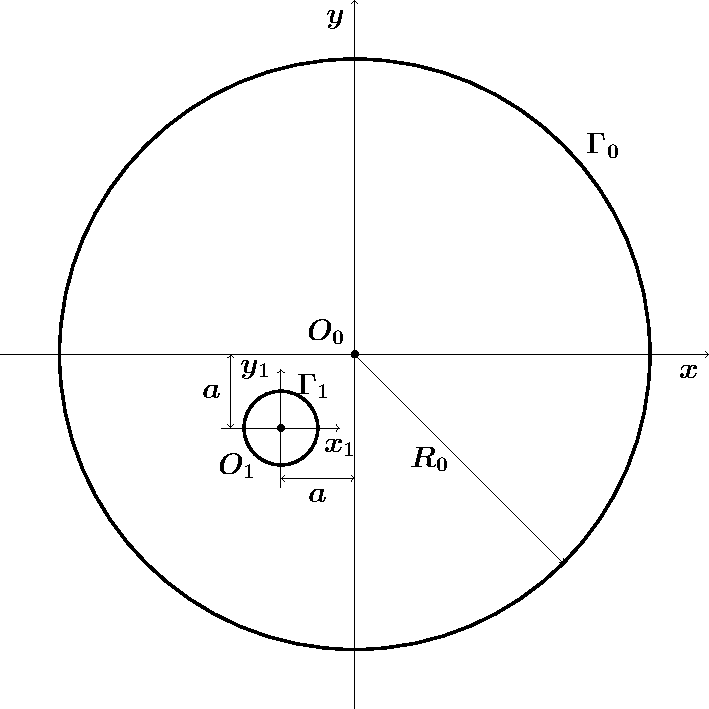
\includegraphics[width=7.5cm]{cav1.pdf}
\caption{\centering Одиночная полость в цилиндрическом образце}
\label{f:7:7}
}{На рис.~\ref{f:7:8} представлены графики распределения напряжений $\sigma_\rho/T$ на диаметре цилиндрического образца, проходящего через центр полости вне ее границы в плоскостях $z=0$, $z=h/2$ и $z=h$ при фиксированных параметрах $\sigma=0.38$, $R_0=10R$, $h/R_0=0.5$; линиям 1, 2, 3 соответствуют графики напряжений в плоскостях $z=0$, $z=h/2$ и $z=h$ на большей части диаметра, а линиям 4, 5, 6~--- на меньшей части. Отрезок $[0,1]$ на оси $Ox$ на графике задает относительное расстояние между точками, соединяющими граничные поверхности внешнего цилиндра и полости на рис.~\ref{f:7:7}. Из анализа графиков, приведенных на рис.~\ref{f:7:8}, можно сделать вывод,} что выполняются граничные условия на цилиндрической полости, свободной от нагрузок по условию задачи, и на внешней границе цилиндра, где приложена кусочно-постоянная нормальная нагрузка.

\begin{figure}
\centering\footnotesize
\parbox[b]{7.5cm}{\centering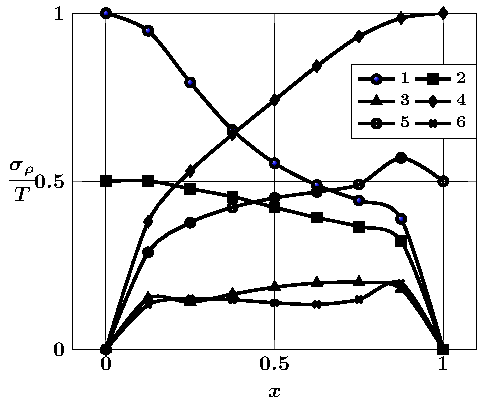
\includegraphics[width=7.5cm]{image-1.pdf}
\caption{Напряжения $\sigma_\rho/T$ для конфигурации, представленной на~рис.~\ref{f:7:7}
\label{f:7:8}}}\hfil\hfil
\parbox[b]{7.5cm}{\centering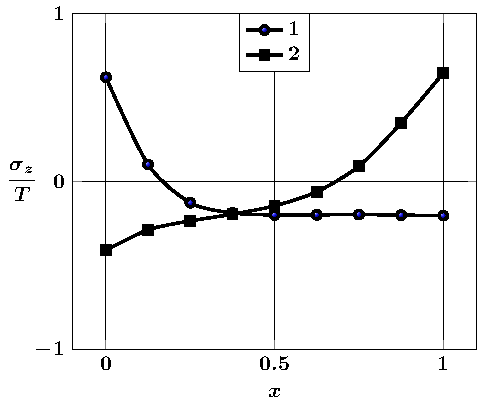
\includegraphics[width=7.5cm]{image-1-z.pdf}
\caption{Напряжения $\sigma_z/T$ для конфигурации, представленной на~рис.~\ref{f:7:7}
\label{f:7:9}}}
\end{figure}

На рис.~\ref{f:7:8} представлены графики распределения напряжений $\sigma_\rho/T$ на диаметре цилиндрического образца, проходящего через центр полости вне ее границы в плоскостях $z=0$, $z=h/2$ и $z=h$ при фиксированных параметрах $\sigma=0.38$, $R_0=10R$, $h/R_0=0.5$; линиям 1, 2, 3 соответствуют графики напряжений в плоскостях $z=0$, $z=h/2$ и $z=h$ на большей части диаметра, а линиям 4, 5, 6~--- на меньшей части. Отрезок $[0,1]$ на оси $Ox$ на графике задает относительное расстояние между точками, соединяющими граничные поверхности внешнего цилиндра и полости на рис.~\ref{f:7:7}. Из анализа графиков, приведенных на рис.~\ref{f:7:8}, можно сделать вывод, что выполняются граничные условия на цилиндрической полости, свободной от нагрузок по условию задачи, и на внешней границе цилиндра, где приложена кусочно-постоянная нормальная нагрузка.

На рис.~\ref{f:7:9} представлены графики распределения напряжений $\sigma_z/T$ на диаметре цилиндрического образца, проходящего через центр полости вне ее границы в плоскости $z=0$ при фиксированных параметрах $\sigma=0.38$, $R_0=10R$, $h/R_0=0.5$; линия 1 соответствует графику на большей части диаметра, линия 2~--- на меньшей части.

\subsection{Две полости в цилиндрическом образце}

На рис.~\ref{f:7:83}, \ref{f:7:85}, \ref{f:7:87}, \ref{f:7:89}, \ref{f:7:91}, \ref{f:7:93}, \ref{f:7:11}, \ref{f:7:12} представлены нормальные компоненты тензора напряжений в декартовых координатах на оси, соединяющей пару цилиндрических полостей (рис.~\ref{f:7:10a}). Фиксированными являются параметры $\sigma=0.38$, $R_0=10R$, $a/R=2.0$, полости сдвинуты относительно центра цилиндрического образца на величину $a$ вдоль осей $x$ и $y$. Изменяется параметр приложенной к образцу нормальной внешней нагрузки $h/R_0=0.5$ и $h/R_0=1.0$.

Из анализа графиков, представленных на рис.~\ref{f:7:11}, можно сделать вывод, что выполняются граничные условия на цилиндрических полостях.

Максимальные по модулю напряжения наблюдаются в средней точке отрезка для напряжений $\sigma_x/T$ и $\sigma_z/T$ и на концах отрезка, т.~е. на границе цилиндров, для напряжений $\sigma_y/T$. Таким образом, основная концентрация напряжений наблюдается на границах полостей, на площадках, к ним перпендикулярных. Следует отметить, что увеличение интенсивности приложенной внешней нагрузки в два раза не приводит к аналогичному увеличению нормальных напряжений: напряжения $\sigma_y/T$ увеличиваются в среднем примерно в полтора раза, напряжения $\sigma_x/T$ по максимальной величине~--- менее чем в два раза, напряжения $\sigma_z/T$ практически не меняются при этом. 

Таким образом, определяющими для напряженного состояния данного образца при данных нагрузках являются напряжения $\sigma_y/T$, максимальные величины которых почти в два раза превышают интенсивность приложенной внешней нагрузки.

Косвенным элементом верификации полученных результатов может служить симметричный характер кривых при симметричных граничных условиях задачи.

\begin{figure}
\centering\footnotesize
\parbox[b]{7.5cm}{\centering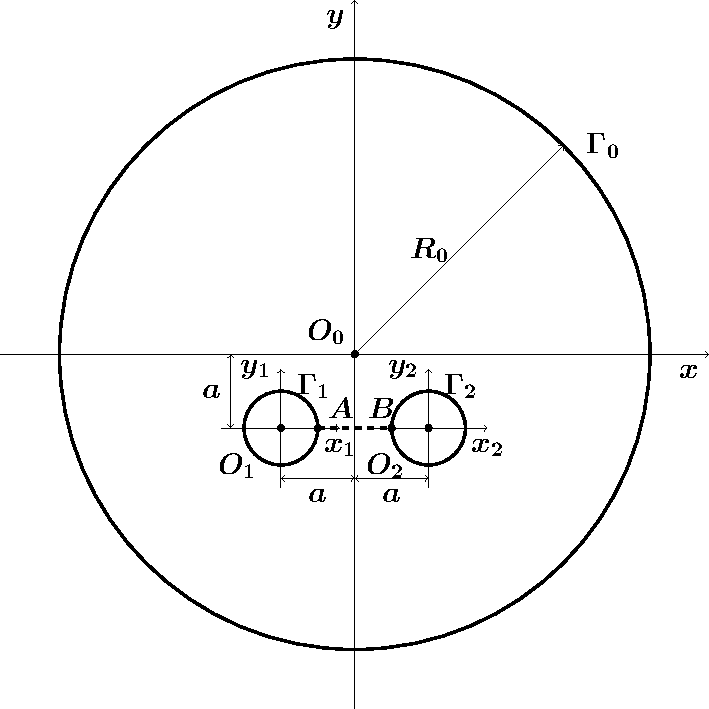
\includegraphics[width=7.5cm]{cav2a.pdf}
\caption{Две полости в цилиндрическом образце, симметричные относительно оси $O_0y$ (конфигурация I)
\label{f:7:10a}}}\hfil\hfil
\parbox[b]{7.5cm}{\centering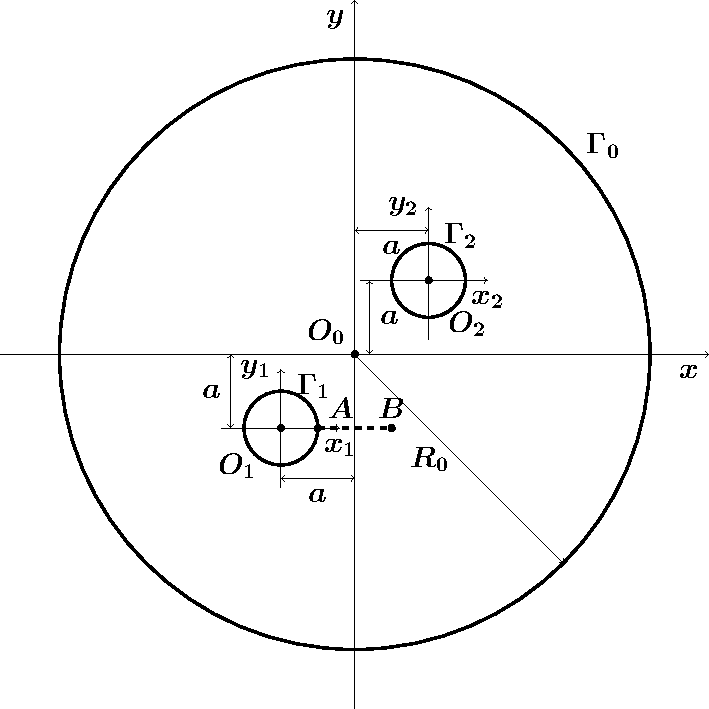
\includegraphics[width=7.5cm]{cav2b.pdf}
\caption{Две центрально симметричные полости в цилиндрическом образце (конфигурация II)
\label{f:7:10b}}}
\end{figure}

\begin{figure}
\centering\footnotesize
\parbox[b]{7.5cm}{\centering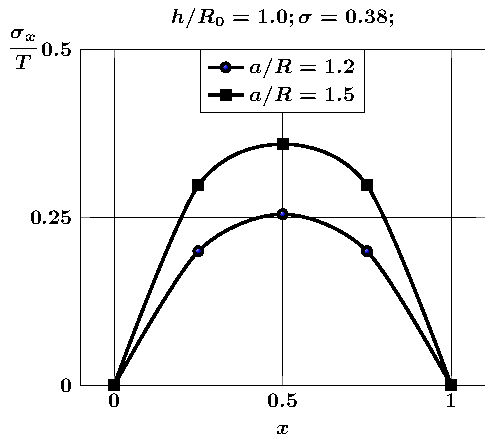
\includegraphics[width=7.5cm]{cav2-a-h10-r10-z0-sig_x.pdf}
\caption{Распределение напряжений $\sigma_x/T$ на линии $AB$ в зависимости от относительного расстояния между полостями в плоскости $z=0$ в конфигурации I
\label{f:7:83}}}\hfil\hfil
\parbox[b]{7.5cm}{\centering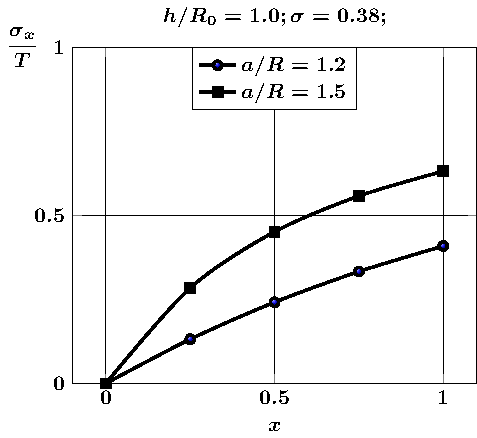
\includegraphics[width=7.5cm]{cav2a-a-h10-r10-z0-sig_x.pdf}
\caption{Распределение напряжений $\sigma_x/T$ на линии $AB$ в зависимости от относительного расстояния между полостями в плоскости $z=0$ в конфигурации II
\label{f:7:84}}}
\end{figure}

\begin{figure}
\centering\footnotesize
\parbox[b]{7.5cm}{\centering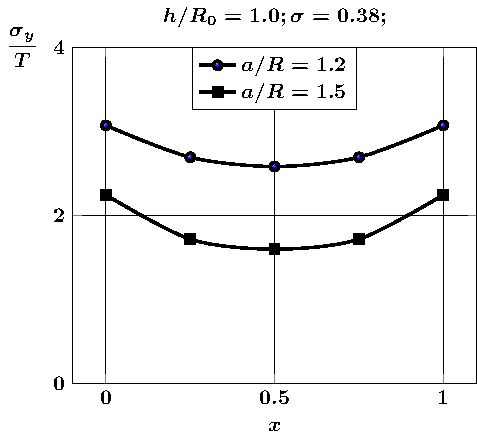
\includegraphics[width=7.5cm]{cav2-a-h10-r10-z0-sig_y.pdf}
\caption{Распределение напряжений $\sigma_y/T$ на линии $AB$ в зависимости от относительного расстояния между полостями в плоскости $z=0$ в конфигурации I
\label{f:7:85}}}\hfil\hfil
\parbox[b]{7.5cm}{\centering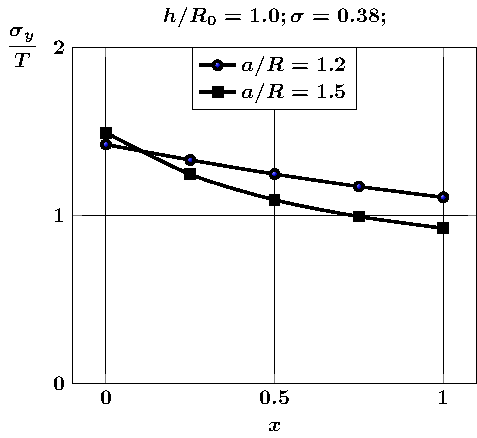
\includegraphics[width=7.5cm]{cav2a-a-h10-r10-z0-sig_y.pdf}
\caption{Распределение напряжений $\sigma_y/T$ на линии $AB$ в зависимости от относительного расстояния между полостями в плоскости $z=0$ в конфигурации II
\label{f:7:86}}}
\end{figure}

\begin{figure}
\centering\footnotesize
\parbox[b]{7.5cm}{\centering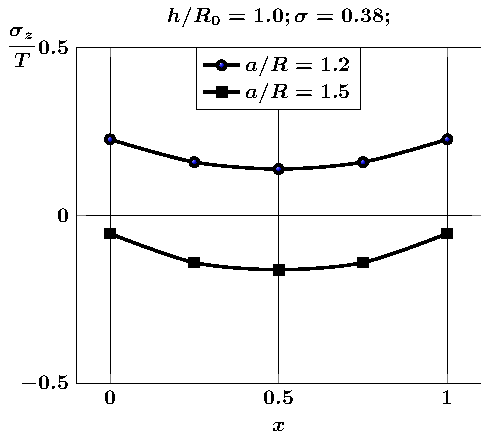
\includegraphics[width=7.5cm]{cav2-a-h10-r10-z0-sig_z.pdf}
\caption{Распределение напряжений $\sigma_z/T$ на линии $AB$ в зависимости от относительного расстояния между полостями в плоскости $z=0$ в конфигурации I
\label{f:7:87}}}\hfil\hfil
\parbox[b]{7.5cm}{\centering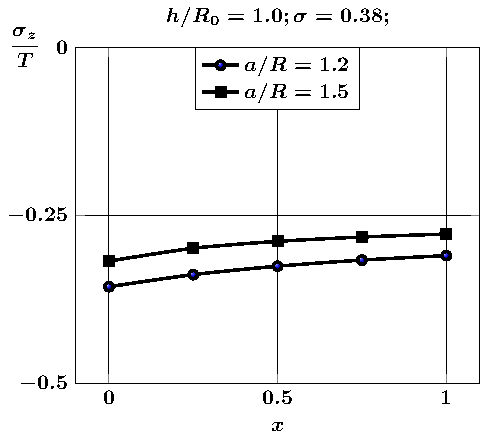
\includegraphics[width=7.5cm]{cav2a-a-h10-r10-z0-sig_z.pdf}
\caption{Распределение напряжений $\sigma_z/T$ на линии $AB$ в зависимости от относительного расстояния между полостями в плоскости $z=0$ в конфигурации II
\label{f:7:88}}}
\end{figure}

\begin{figure}
\centering\footnotesize
\parbox[b]{7.5cm}{\centering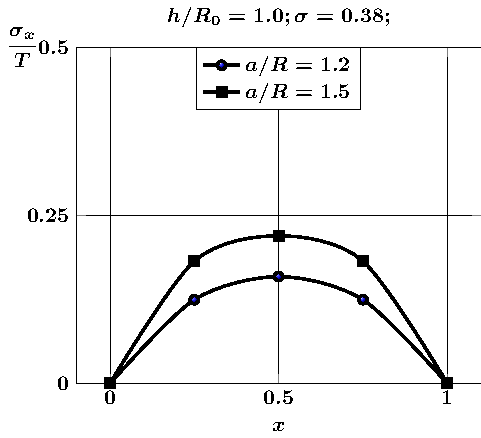
\includegraphics[width=7.5cm]{cav2-a-h10-r10-z1-sig_x.pdf}
\caption{Распределение напряжений $\sigma_x/T$ на линии $AB$ в зависимости от относительного расстояния между полостями в плоскости $z=h/2$ в конфигурации I
\label{f:7:89}}}\hfil\hfil
\parbox[b]{7.5cm}{\centering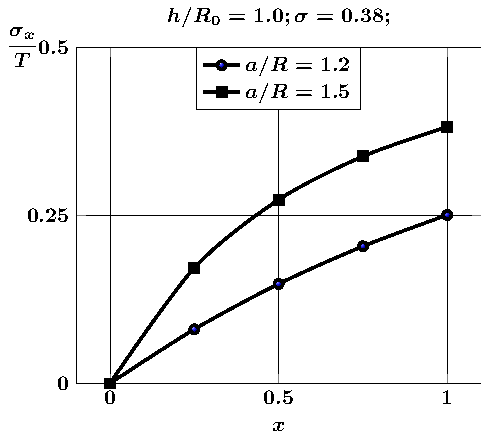
\includegraphics[width=7.5cm]{cav2a-a-h10-r10-z1-sig_x.pdf}
\caption{Распределение напряжений $\sigma_x/T$ на линии $AB$ в зависимости от относительного расстояния между полостями в плоскости $z=h/2$ в конфигурации II
\label{f:7:90}}}
\end{figure}

\begin{figure}
\centering\footnotesize
\parbox[b]{7.5cm}{\centering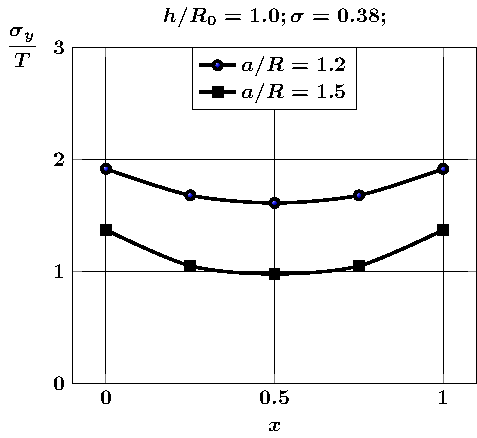
\includegraphics[width=7.5cm]{cav2-a-h10-r10-z1-sig_y.pdf}
\caption{Распределение напряжений $\sigma_y/T$ на линии $AB$ в зависимости от относительного расстояния между полостями в плоскости $z=h/2$ в конфигурации I
\label{f:7:91}}}\hfil\hfil
\parbox[b]{7.5cm}{\centering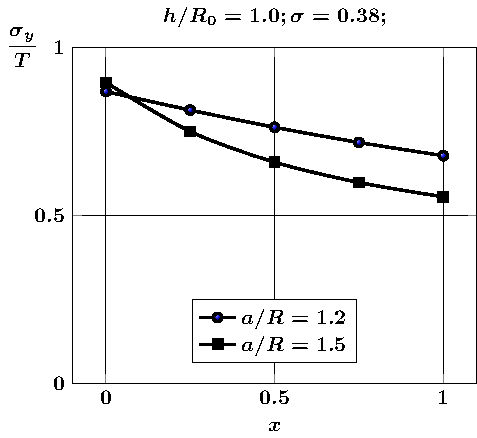
\includegraphics[width=7.5cm]{cav2a-a-h10-r10-z1-sig_y.pdf}
\caption{Распределение напряжений $\sigma_y/T$ на линии $AB$ в зависимости от относительного расстояния между полостями в плоскости $z=h/2$ в конфигурации II
\label{f:7:92}}}
\end{figure}

\begin{figure}
\centering\footnotesize
\parbox[b]{7.5cm}{\centering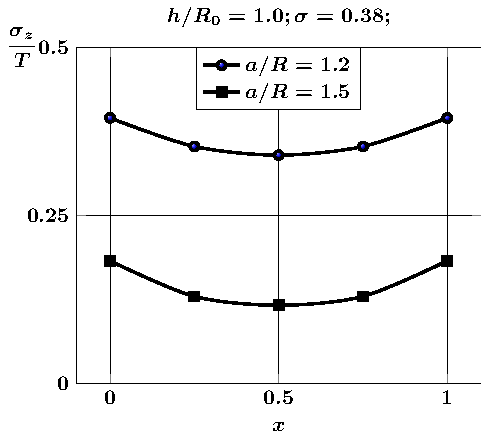
\includegraphics[width=7.5cm]{cav2-a-h10-r10-z1-sig_z.pdf}
\caption{Распределение напряжений $\sigma_z/T$ на линии $AB$ в зависимости от относительного расстояния между полостями в плоскости $z=h/2$ в конфигурации I
\label{f:7:93}}}\hfil\hfil
\parbox[b]{7.5cm}{\centering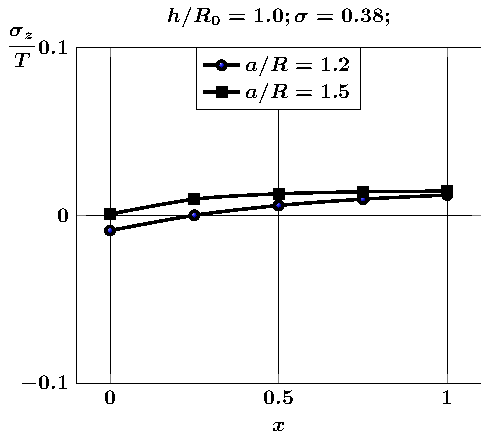
\includegraphics[width=7.5cm]{cav2a-a-h10-r10-z1-sig_z.pdf}
\caption{Распределение напряжений $\sigma_z/T$ на линии $AB$ в зависимости от относительного расстояния между полостями в плоскости $z=h/2$ в конфигурации II
\label{f:7:94}}}
\end{figure}

\begin{figure}
\centering\footnotesize
\parbox[b]{7.5cm}{\centering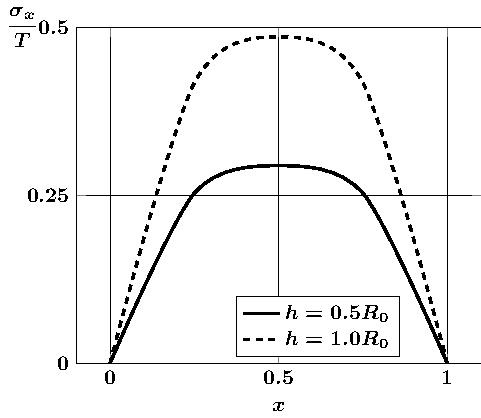
\includegraphics[width=7.5cm]{image-2-x.pdf}
\caption{Напряжения $\sigma_x/T$ на линии $AB$ в зависимости от $h/R_0$ для конфигурации I
\label{f:7:11}}}\hfil\hfil
\parbox[b]{7.5cm}{\centering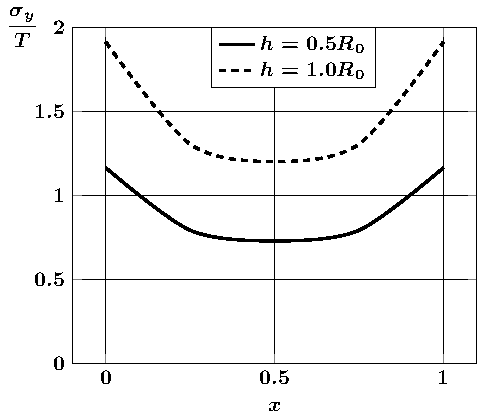
\includegraphics[width=7.5cm]{image-2-y.pdf}
\caption{Напряжения $\sigma_y/T$ на линии $AB$ в зависимости от $h/R_0$ для конфигурации I
\label{f:7:12}}}
\end{figure}

%\begin{figure}
%\centering
%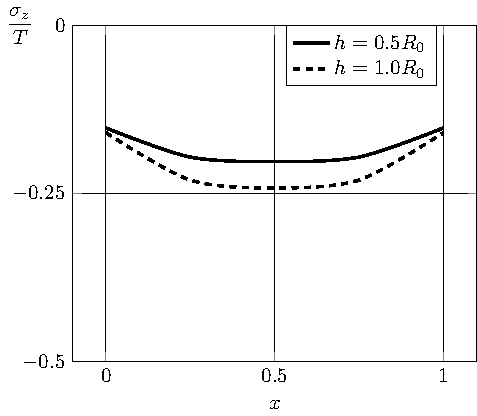
\includegraphics[width=12cm]{image-2-z.pdf}
%\caption{Относительные напряжения $\sigma_z/T$ для конфигурации, представленной на рис.~\ref{f:7:10} в зависимости от изменения параметра $h/R_0$}
%\label{f:7:13}
%\end{figure}

\subsection{Тетрагональная структура расположения полостей в~цилиндрическом образце}

Рассмотрим цилиндрический образец пористого материала с тетрагональной структурой расположения полостей, как представлено на рис.~\ref{f:7:6}. Вычисления проведены при фиксированных параметрах $\sigma=0.38$, $h/R_0=1.0$, $R_0=10R$ в плоскости $z=0$. Каждая из полостей сдвинута относительно центра цилиндрического образца вдоль осей $x$ и $y$ на величину $a$. Относительное расстояние между цилиндрическими полостями изменялось следующим образом: $a/R=2.0$, $a/R=1.5$ и $a/R=1.2$, что соответствует пористости материала $\zeta=0.1964$, $\zeta=0.3491$ и $\zeta=0.5454$.

На рис.~\ref{f:7:15} приведены относительные напряжения $\sigma_x/T$ на линии, соединяющей центры соседних полостей для конфигурации, представленной на рис.~\ref{f:7:6} в зависимости от изменения относительного расстояния между полостями. Из графиков, приведенных на рис.~\ref{f:7:15}, видно, что граничные условия на полостях выполняются для всех значений параметра $a/R$, а также падает концентрация напряжений $\sigma_x/T$ в средней точке отрезка при приближении полостей друг к другу.

\begin{figure}[h!]
\centering\footnotesize
\parbox[b]{7.5cm}{\centering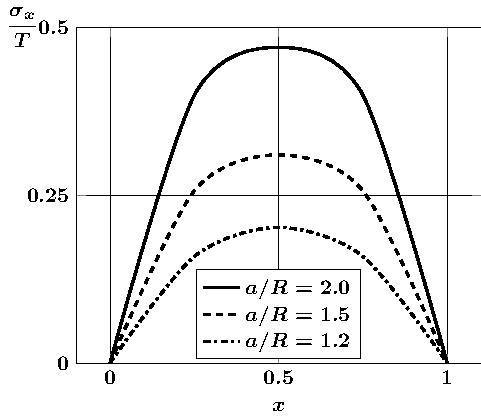
\includegraphics[width=7.5cm]{cav4_sig-x.pdf}
\caption{Напряжения $\sigma_x/T$ на линии $AB$ для конфигурации, представленной на рис.~\ref{f:7:6}, в зависимости от относительного расстояния между полостями
\label{f:7:15}}}\hfil\hfil
\parbox[b]{7.5cm}{\centering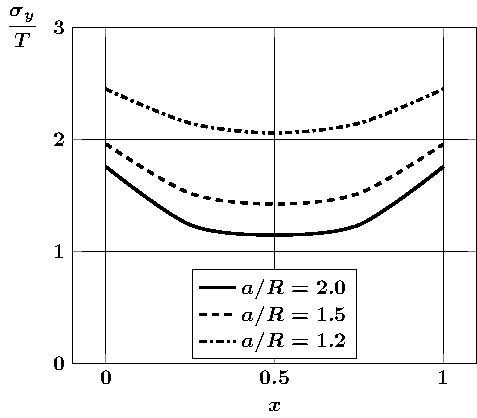
\includegraphics[width=7.5cm]{cav4_sig-y.pdf}
\caption{Напряжения $\sigma_y/T$ на линии $AB$ для конфигурации, представленной на рис.~\ref{f:7:6}, в зависимости от относительного расстояния между полостями
\label{f:7:16}}}
\end{figure}

На рис.~\ref{f:7:16} приведены относительные напряжения $\sigma_y/T$ на линии, соединяющей центры соседних полостей для конфигурации, представленной на рис.~\ref{f:7:6}, в зависимости от изменения относительного расстояния между полостями. Из графиков, приведенных на рис.~\ref{f:7:16}, видно, что растет концентрация напряжений $\sigma_y/T$ у смежных полюсов цилиндров при приближении полостей друг к другу. Следует также обратить внимание, что при достаточно высокой пористости материала (более 50~\%) максимальные по величине относительные напряжения $\sigma_y/T$ могут в 2.5 раза превосходить интенсивность внешних нагрузок, приложенных к образцу.

На рис.~\ref{f:7:17} приведены относительные напряжения $\sigma_z/T$ на линии, соединяющей центры соседних полостей для конфигурации, представленной на рис.~\ref{f:7:6}, в зависимости от изменения относительного расстояния между полостями. Из графиков, приведенных на рис.~\ref{f:7:17}, видно, что напряжения $\sigma_z/T$ в несколько раз уменьшаются по абсолютной величине при приближении полостей друг к другу. При этом характер кривых сохраняется. Характерным также является то, что относительные напряжения $\sigma_z/T<0$ на всем рассматриваемом отрезке, то есть цилиндрический образец пористого материала в данном случае сжимается в продольном направлении.

\sidefig(75mm){
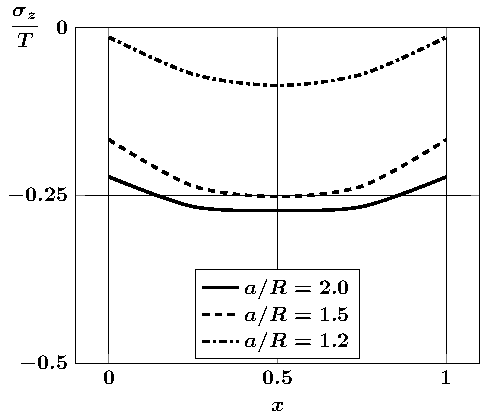
\includegraphics[width=7.5cm]{cav4_sig-z.pdf}
\caption{Напряжения $\sigma_y/T$ на линии $AB$ для конфигурации, представленной на рис.~\ref{f:7:6}, в зависимости от относительного расстояния между полостями}
\label{f:7:17}
}{В табл.~\ref{t:7:4} приведены данные проверки граничных условий на одной из полостей в тетрагональной структуре при $R_0=10R$, $h/R_0=1.0$, $a/R=1.2$ и $m_{max}=20$, то есть в бесконечных суммах удерживаем 41 слагаемое. Из анализа приведенных данных видно, что граничные условия на полостях при близком их расположении в тетрагональной структуре выполняются достаточно хорошо.

На рис.~\ref{f:7:27} представлена тетрагональная структура расположения полостей в цилиндрическом образце с шестнадцатью полостями.
}

\begin{table}[h!]
\caption{Проверка граничных условий}
\centering
$
\begin{array}{|c|c|c|c|c|}
\hline
\varphi & 0 & \dfrac{\pi}{2} & \pi & \dfrac{3\pi}{2} \\
\hline
\sigma_\rho & -4.42278\times10^{-6} & -4.4263\times10^{-6} & 2.43255\times 10^{-6} & 2.42862\times 10^{-6} \\
\hline
\end{array}
$
\label{t:7:4}
\end{table}

На рис.~\ref{f:7:28}~--- \ref{f:7:30} представлены графики напряжений $\sigma_x/T$, $\sigma_y/T$ и $\sigma_z/T$ на линии, соединяющей центры соседних полостей для конфигурации, представленной на рис.~\ref{f:7:27}, в зависимости от изменения относительного расстояния между полостями в плоскостях $z=0$ и $z=h$. Из анализа данных графиков можно сделать вывод, что при приближении полостей концентрация напряжений $\sigma_y/T$ растет, а напряжения $\sigma_x/T$ уменьшаются как в плоскости $z=0$, так и в плоскости $z=h$. При переходе от плоскости $z=0$ к плоскости $z=h$ величины нормальных напряжений $\sigma_x/T$ и $\sigma_y/T$ уменьшаются, а напряжения $\sigma_z/T$ меняют знаки с отрицательных на положительные.

В табл.~\ref{t:7:5} приведены данные о сходимости метода редукции для случая шестнадцати полостей в тетрагональной структуре при $a/R=1.5$ и $h/R_0=1.0$ в средней точке отрезка $AB$. Данные таблицы говорят о том, что удовлетворительную точность можно получить уже при $m_{max}=5$.

\sidefig(75mm){
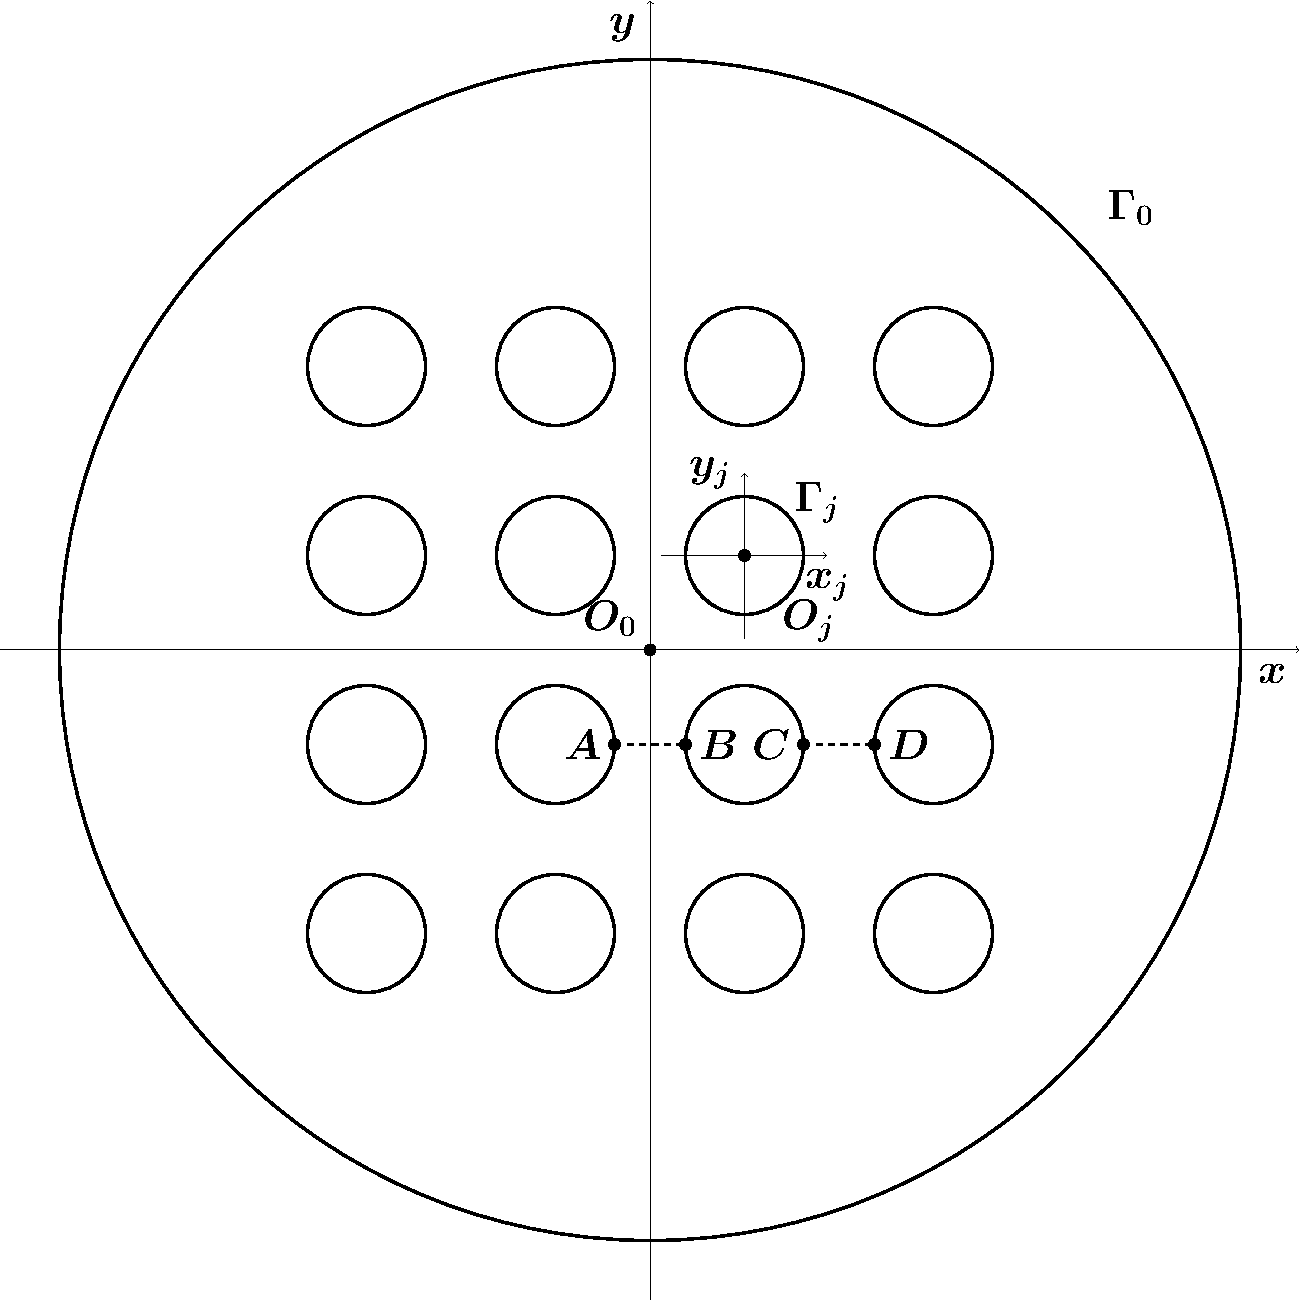
\includegraphics[width=7.5cm]{tetragonal-16.pdf}
\caption{Тетрагональная структура расположения полостей в цилиндрическом образце с шестнадцатью полостями}
\label{f:7:27}
}{На рис.~\ref{f:7:31} приведен график относительного напряжения $\sigma_y/T$ на линии, соединяющей центры соседних полостей, для конфигурации, представленной на рис.~\ref{f:7:27}, в зависимости от изменения интенсивности приложенной внешней нагрузки $h/R_0$ в плоскостях $z=0$ и $z=h$. График распределения напряжений $\sigma_y/T$ показывает, что области концентрации напряжений находятся вблизи границ полостей. При увеличении ширины кольца приложения внешней нормальной нагрузки в два раза напряжения $\sigma_y/T$ на линии $AB$ в плоскости $z=0$ увеличиваются более чем в полтора раза.\par\sloppy
}

\begin{figure}[h!]
\centering\footnotesize
\parbox[b]{7.5cm}{\centering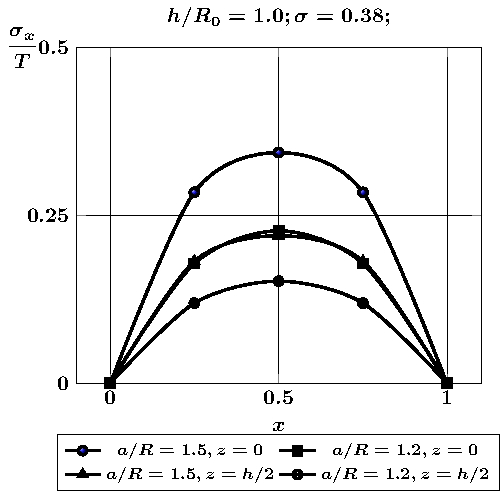
\includegraphics[width=7.5cm]{cav16-sig_x.pdf}
\caption{Напряжения $\sigma_x/T$ на линии $AB$ для конфигурации, представленной на рис.~\ref{f:7:27}, в зависимости от относительного расстояния между полостями в плоскостях $z=0$ и $z=h/2$
\label{f:7:28}}}\hfil\hfil
\parbox[b]{7.5cm}{\centering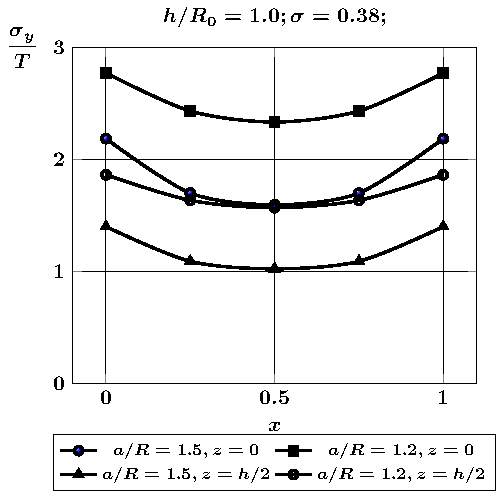
\includegraphics[width=7.5cm]{cav16-sig_y.pdf}
\caption{Напряжения $\sigma_y/T$ на линии $AB$ для конфигурации, представленной на рис.~\ref{f:7:27}, в зависимости от относительного расстояния между полостями в плоскостях $z=0$ и $z=h/2$
\label{f:7:29}}}
\end{figure}

\begin{figure}[h!]
\centering\footnotesize
\parbox[b]{7.5cm}{\centering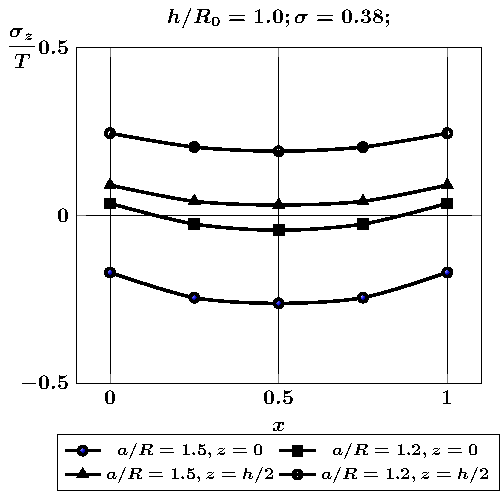
\includegraphics[width=7.5cm]{cav16-sig_z.pdf}
\caption{Напряжения $\sigma_z/T$ на линии $AB$ для конфигурации, представленной на рис.~\ref{f:7:27}, в зависимости от относительного расстояния между полостями в плоскостях $z=0$ и $z=h/2$
\label{f:7:30}}}\hfil\hfil
\parbox[b]{7.5cm}{\centering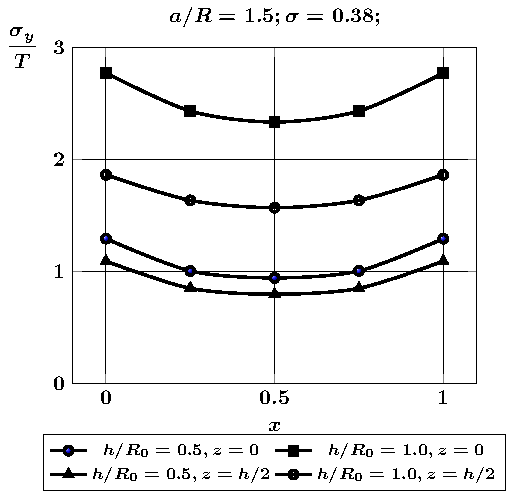
\includegraphics[width=7.5cm]{cav16-h-sig_y.pdf}
\caption{Напряжения $\sigma_y/T$ на линии $AB$ для конфигурации, представленной на рис.~\ref{f:7:27}, в зависимости от интенсивности приложенной внешней нагрузки $h/R_0$ в плоскостях $z=0$ и $z=h/2$
\label{f:7:31}}}
\end{figure}

\begin{figure}[h!]
\centering\footnotesize
\parbox[b]{7.5cm}{\centering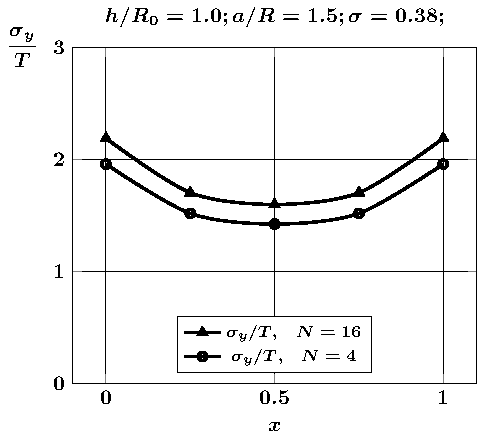
\includegraphics[width=7.5cm]{cav16-4-sig_y.pdf}
\caption{Напряжения $\sigma_y/T$ на линии $AB$ для конфигураций, представленных на рис.~\ref{f:7:6} и~\ref{f:7:27}, в зависимости от количества полостей в тетрагональной структуре
\label{f:7:32}}}\hfil\hfil
\parbox[b]{7.5cm}{\centering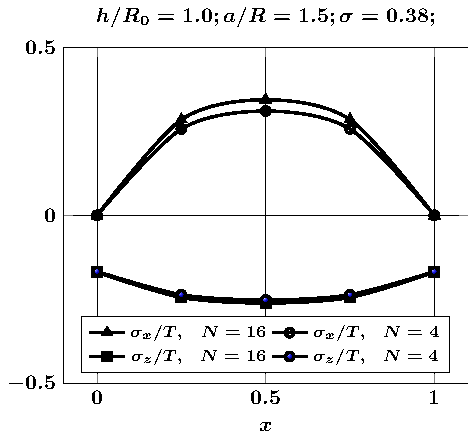
\includegraphics[width=7.5cm]{cav16-4-sig_x_z.pdf}
\caption{Напряжения $\sigma_x/T$ и $\sigma_z/T$ на линии $AB$ для конфигураций, представленных на рис.~\ref{f:7:6} и~\ref{f:7:27}, в зависимости от количества полостей в тетрагональной структуре
\label{f:7:33}}}
\end{figure}

\begin{table}[h!]
\caption{Сходимость метода редукции для случая шестнадцати полостей}
\centering
\begin{tabular}{|c|c|c|c|c|}
\hline
$m_{max}$ & 5 & 10 & 15 & 20 \\
\hline
$\sigma_x/T$ & $0.343729$ & $0.344384$ & $0.344381$ & $0.344382$ \\
\hline
$\sigma_y/T$ & $1.5964$ & $1.59645$ & $1.59648$ & $1.59648$ \\
\hline
$\sigma_z/T$ & $-0.260994$ & $-0.260695$ & $-0.260671$ & $-0.260669$ \\
\hline
\end{tabular}
\label{t:7:5}
\end{table}

На рис.~\ref{f:7:32} и~\ref{f:7:33} приведены графики напряжений $\sigma_x/T$, $\sigma_y/T$ и $\sigma_z/T$ на линии, соединяющей центры соседних полостей, для конфигураций, представленных на рис.~\ref{f:7:6} и~\ref{f:7:27}, в зависимости от количества полостей в тетрагональной структуре. Можно сделать вывод, что значения напряжений $\sigma_x/T$ и $\sigma_z/T$ и их распределения на линии $AB$ практически не зависят от числа полостей, в то время как напряжения $\sigma_y/T$ в случае шестнадцати полостей увеличиваются примерно на 10~\%. Характер распределения напряжений от числа полостей не зависит. Приведенные данные позволяют использовать локальные модели при описании напряженно-деформированного состояния пористого материала с параллельными цилиндрическими порами.

\subsection{Тетрагональная объемно центрированная структура расположения полостей в цилиндрическом образце}

\sidefig(75mm){
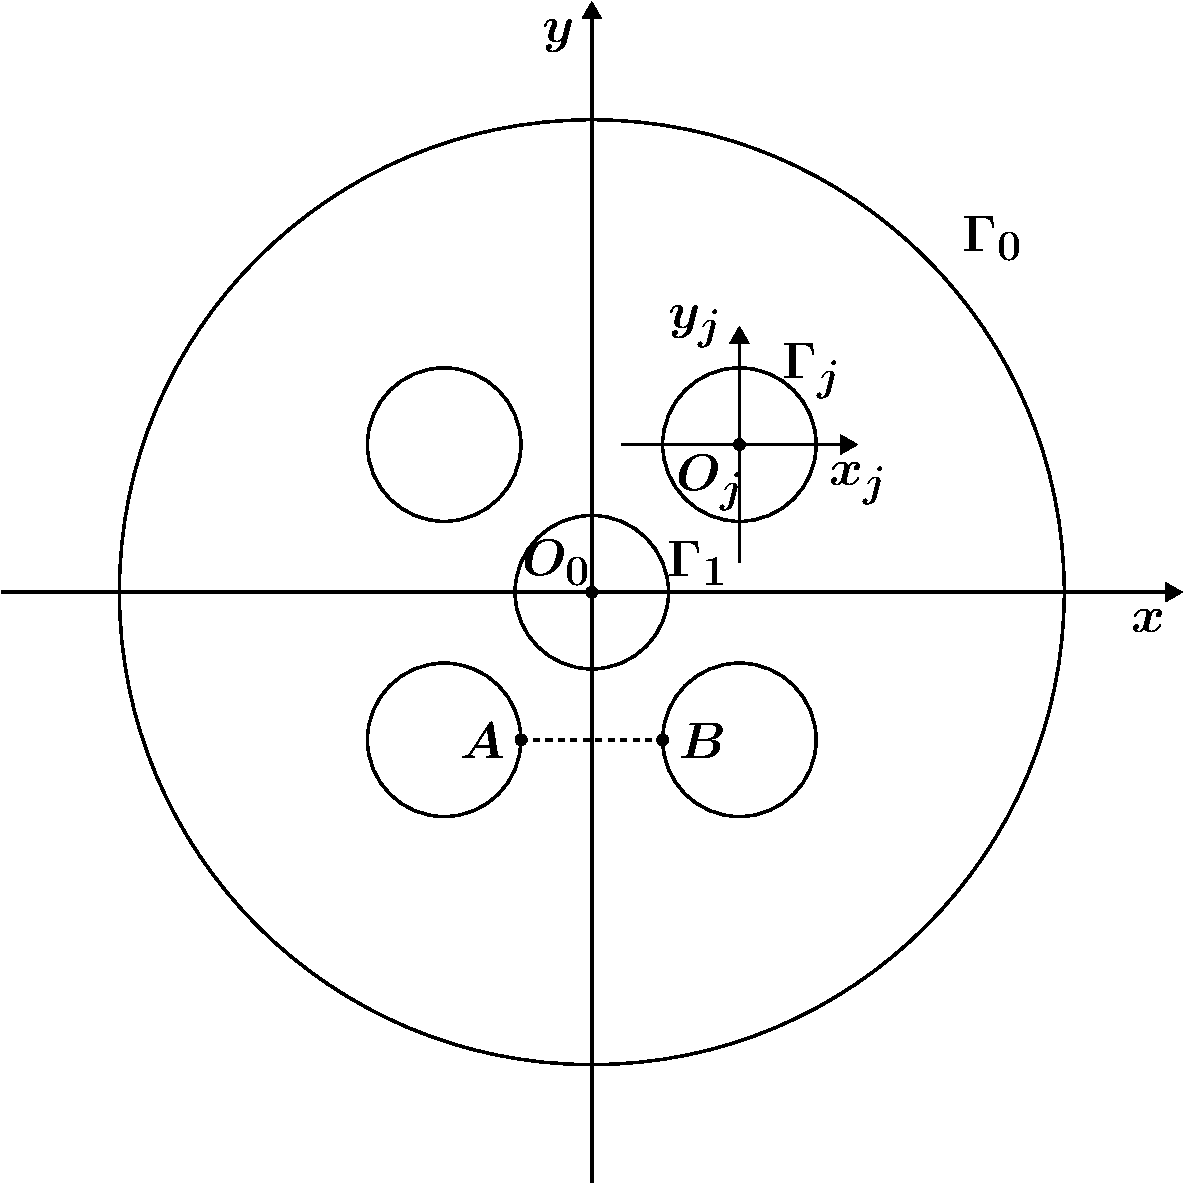
\includegraphics[width=7.5cm]{tetragonal-centroid.pdf}
\caption{Тетрагональная объемно центрированная структура расположения полостей в цилиндрическом образце}
\label{f:7:18}
}{Рассмотрим тетрагональную объемно центрированную структуру расположения полостей в цилиндрическом образце, представленную на рис.~\ref{f:7:18}. Компьютерный эксперимент показывает качественно иной характер в распределении напряжений при переходе от тетрагональной упаковки к объемно центрированному ее варианту. Поэтому изучение такого вида упаковки является важным для оптимального определения геометрических параметров, приводящих к наименьшей концентрации напряжений в теле.
 
Заметим, что формулы~\eqref{eq:7:22}~--- \eqref{eq:7:24} из параграфа 2.2 отражают другую структуру разрешающей системы для определения неизвестных коэффициентов в общем решении.
}

На рис.~\ref{f:7:19} и~\ref{f:7:20} приводится сравнение относительных напряжений $\sigma_x/T$ и $\sigma_y/T$ на линии, соединяющей центры соседних полостей для тетрагональной и центрированной тетрагональной структур при прочих одинаковых параметрах.

\begin{figure}[h!]
\centering\footnotesize
\parbox[b]{7.5cm}{\centering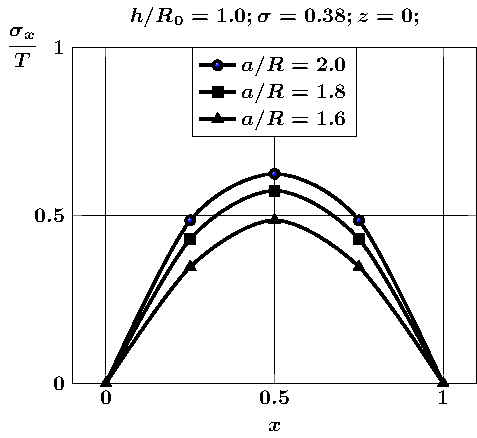
\includegraphics[width=7.5cm]{cav5-a-h10-r10-z0-sig_x.pdf}
\caption{Напряжения $\sigma_x/T$ на линии $AB$ для центрированной тетрагональной структуры в зависимости от относительного расстояния между полостями в плоскости $z=0$ 
\label{f:7:95}}}\hfil\hfil
\parbox[b]{7.5cm}{\centering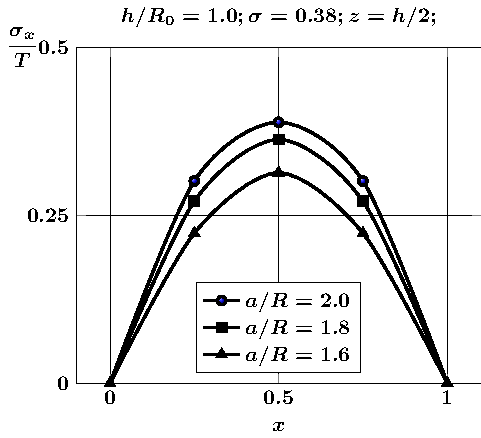
\includegraphics[width=7.5cm]{cav5-a-h10-r10-z1-sig_x.pdf}
\caption{Напряжения $\sigma_x/T$ на линии $AB$ для центрированной тетрагональной структуры в зависимости от относительного расстояния между полостями в плоскости $z=h/2$
\label{f:7:96}}}
\end{figure}

\begin{figure}[h!]
\centering\footnotesize
\parbox[b]{7.5cm}{\centering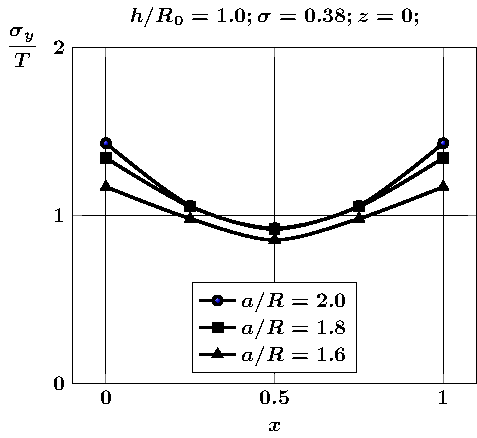
\includegraphics[width=7.5cm]{cav5-a-h10-r10-z0-sig_y.pdf}
\caption{Напряжения $\sigma_y/T$ на линии $AB$ для центрированной тетрагональной структуры в зависимости от относительного расстояния между полостями в плоскости $z=0$ 
\label{f:7:97}}}\hfil\hfil
\parbox[b]{7.5cm}{\centering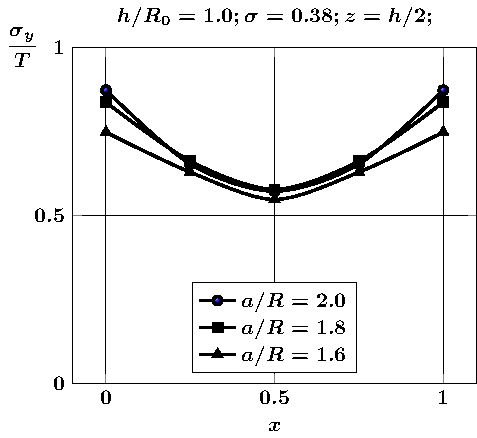
\includegraphics[width=7.5cm]{cav5-a-h10-r10-z1-sig_y.pdf}
\caption{Напряжения $\sigma_y/T$ на линии $AB$ для центрированной тетрагональной структуры в зависимости от относительного расстояния между полостями в плоскости $z=h/2$
\label{f:7:98}}}
\end{figure}

\begin{figure}[h!]
\centering\footnotesize
\parbox[b]{7.5cm}{\centering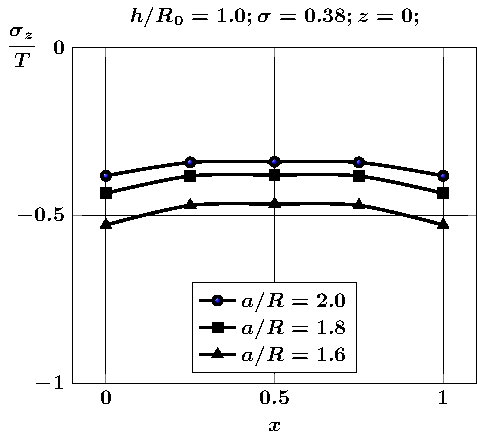
\includegraphics[width=7.5cm]{cav5-a-h10-r10-z0-sig_z.pdf}
\caption{Напряжения $\sigma_z/T$ на линии $AB$ для центрированной тетрагональной структуры в зависимости от относительного расстояния между полостями в плоскости $z=0$ 
\label{f:7:99}}}\hfil\hfil
\parbox[b]{7.5cm}{\centering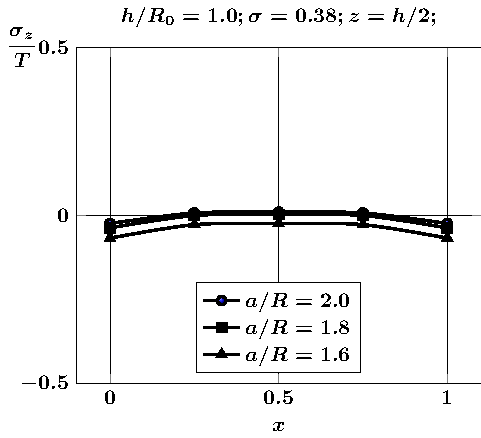
\includegraphics[width=7.5cm]{cav5-a-h10-r10-z1-sig_z.pdf}
\caption{Напряжения $\sigma_z/T$ на линии $AB$ для центрированной тетрагональной структуры в зависимости от относительного расстояния между полостями в плоскости $z=h/2$
\label{f:7:100}}}
\end{figure}

\begin{figure}[h!]
\centering\footnotesize
\parbox[b]{7.5cm}{\centering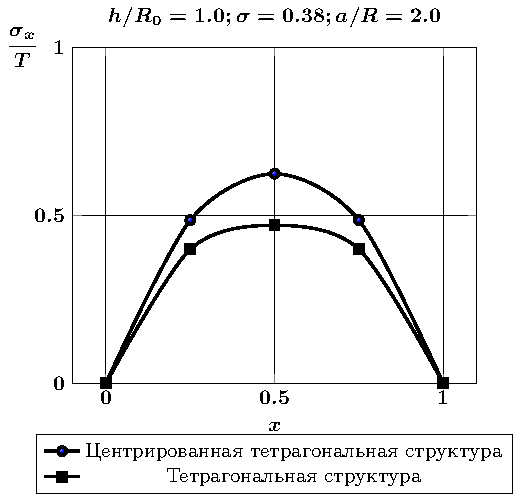
\includegraphics[width=7.5cm]{cav5-4-sig_x.pdf}
\caption{Напряжения $\sigma_x/T$ на линии $AB$ для тетрагональной и центрированной тетрагональной структур
\label{f:7:19}}}\hfil\hfil
\parbox[b]{7.5cm}{\centering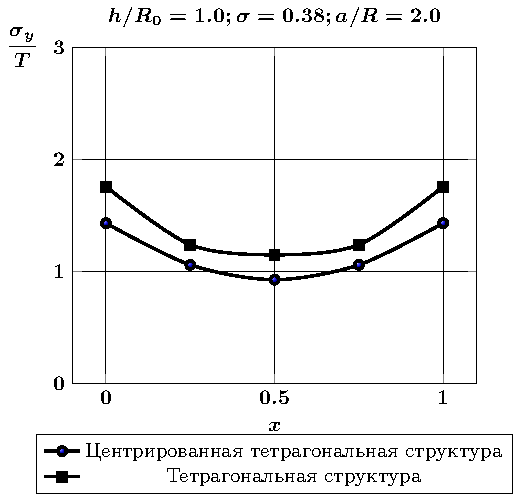
\includegraphics[width=7.5cm]{cav5-4-sig_y.pdf}
\caption{Напряжения $\sigma_y/T$ на линии $AB$ для тетрагональной и центрированной тетрагональной структур
\label{f:7:20}}}
\end{figure}

\subsection{Гексагональная структура расположения полостей в~цилиндрическом образце}

Рассмотрим гексагональную структуру расположения полостей в цилиндрическом образце, представленную на рис.~\ref{f:7:21}. Гексагональная упаковка обладает максимальной степенью симметрии по отношению к упаковкам, рассмотренным ранее. При вычислении эффективных упругих модулей для материала с подобным расположением полостей можно считать, что этот материал обладает трансверсальной изотропией при условии, что на его границе приложено однородное напряженно-деформированное состояние.

\sidefig*(75mm){
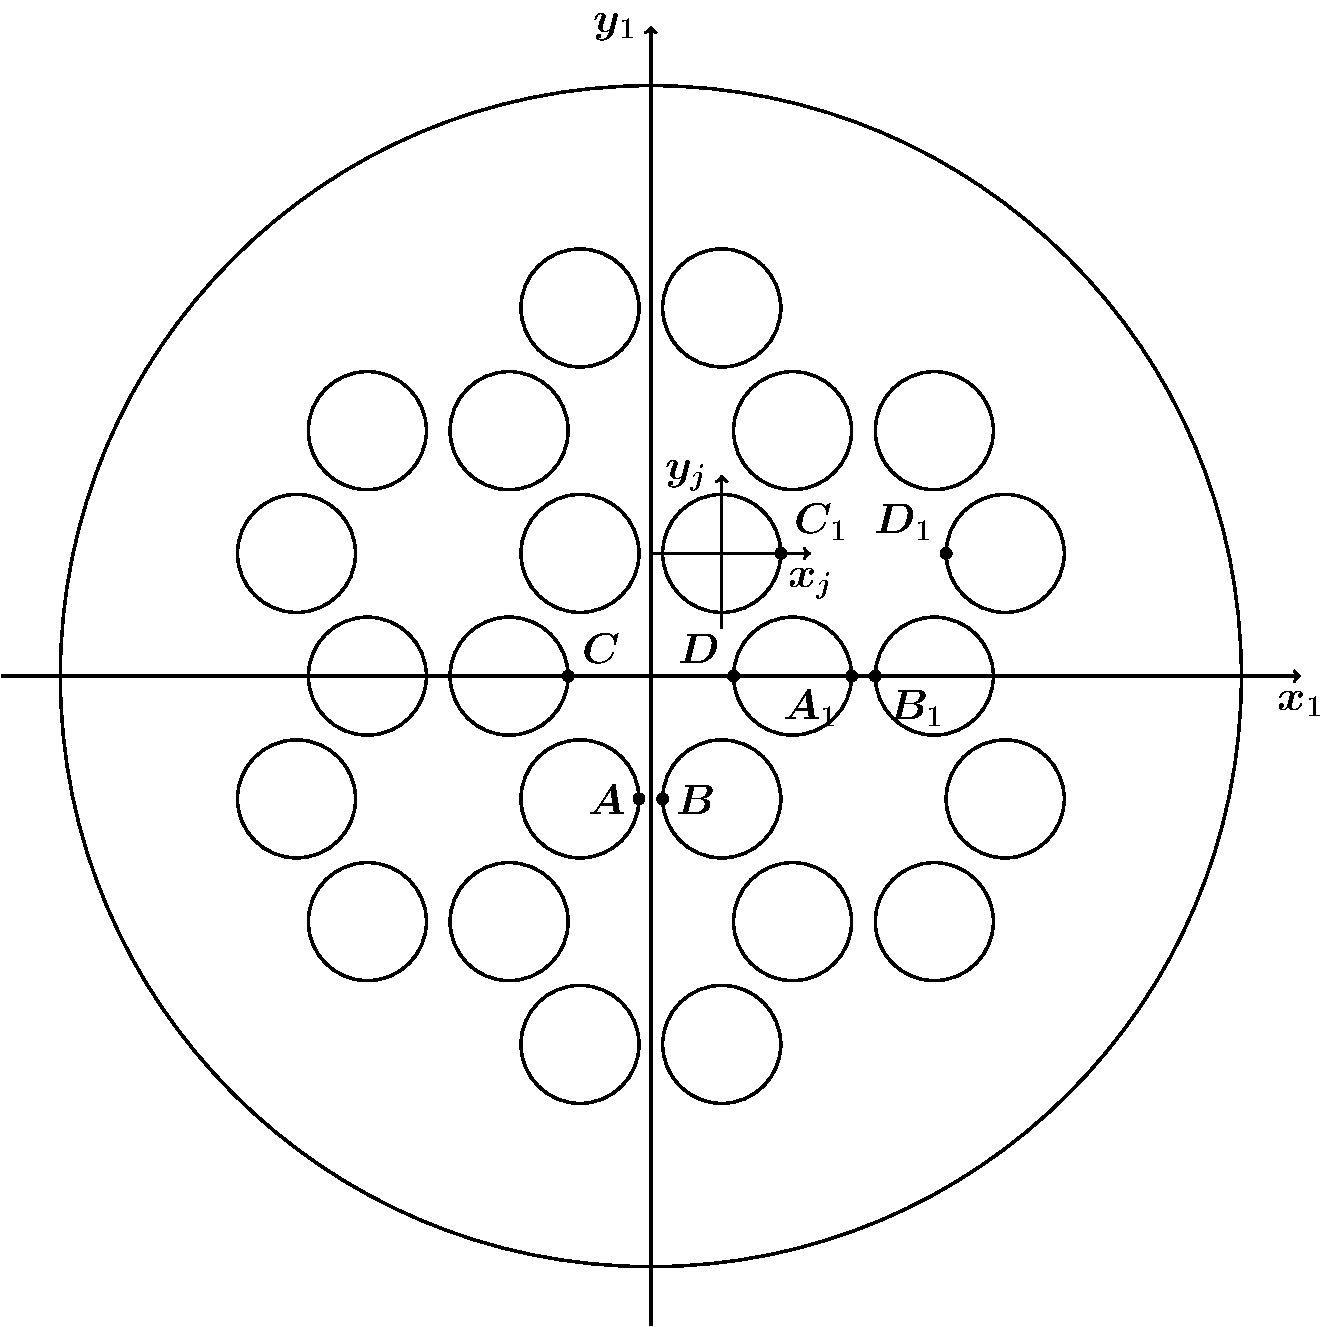
\includegraphics[width=7.5cm]{hexagonal.pdf}
\caption{Гексагональная структура расположения полостей в цилиндрическом образце}
\label{f:7:21}
}{
На рис.~\ref{f:7:126} и \ref{f:7:127} приведены графики нормальных напряжений на линии $AB$ в плоскостях $z=0$ и $z=h/2$ в зависимости от относительного расстояния между полостями. При уменьшении расстояния между полостями наблюдается рост напряжений $\sigma_y/T$. Для напряжений $\sigma_x/T$ наблюдается обратная картина. Напряжения $\sigma_z/T$ при приближении полостей меняют знак с сжимающих на растягивающие. Основной вклад в напряженное состояние вносят напряжения $\sigma_y/T$. На эти напряжения в наибольшей степени оказывает влияние расстояние между полостями.
}

\begin{figure}[h!]
\centering\footnotesize
\parbox[b]{7.5cm}{\centering\includegraphics[width=8cm]{cav24-a-h10-r10-z0.pdf}
\caption{Нормальные напряжения на линии $AB$ в зависимости от относительного расстояния между полостями в плоскости $z=0$
\label{f:7:126}}}\hfil\hfil
\parbox[b]{7.5cm}{\centering\includegraphics[width=8cm]{cav24-a-h10-r10-z1.pdf}
\caption{Нормальные напряжения на линии $AB$ в зависимости от относительного расстояния между полостями в плоскости $z=h/2$
\label{f:7:127}}}
\end{figure}

На рис.~\ref{f:7:128} и \ref{f:7:129} представлены графики нормальных напряжений на линии $CD$ в плоскостях $z=0$ и $z=h/2$ в зависимости от относительного расстояния между полостями. При уменьшении расстояния между полостями наблюдается уменьшение напряжений $\sigma_x/T$ и $\sigma_y/T$. Напряжения $\sigma_z/T$ растут по абсолютной величине при приближении полостей и являются сжимающими вне зависимости от расстояния между ними. В сравнении с отрезком $AB$ напряжения $\sigma_y/T$ на линии $CD$ уменьшаются в среднем в 2--2.5~раза.

\begin{figure}[h!]
\centering\footnotesize
\parbox[b]{7.5cm}{\centering\includegraphics[width=8cm]{cav24-a-h10-r10-z0-diag.pdf}
\caption{Нормальные напряжения на линии $CD$ в зависимости от относительного расстояния между полостями в плоскости $z=0$
\label{f:7:128}}}\hfil\hfil
\parbox[b]{7.5cm}{\centering\includegraphics[width=8cm]{cav24-a-h10-r10-z1-diag.pdf}
\caption{Нормальные напряжения на линии $CD$ в зависимости от относительного расстояния между полостями в плоскости $z=h/2$
\label{f:7:129}}}
\end{figure}

В табл.~\ref{t:7:7} приведены результаты, показывающие скорость сходимости метода редукции для 24 цилиндрических полостей. Сравниваются значения напряжений $\sigma_x/T$, $\sigma_y/T$, $\sigma_z/T$ в средней точке отрезка $AB$ при $m_{max}=\\=10,12,15$, $a/R=1.5$, $h/R_0=1.0$. Метод показал хорошую сходимость уже для $m_{max}=10$.\par\sloppy

\begin{table}[h!]
\caption{Сходимость метода редукции для 24 цилиндрических полостей}
\centering
$
\begin{array}{|c|c|c|c|}
\hline
m_{max} & 10 & 12 & 15 \\
\hline
\sigma_x & 0.441673 & 0.440023 & 0.440023 \\
\hline
\sigma_y & 1.9923 & 1.98469 & 1.98469 \\
\hline
\sigma_z & -0.219197 & -0.219834 & -0.219834 \\
\hline
\end{array}
$
\label{t:7:7}
\end{table}

На рис.~\ref{f:7:130} и \ref{f:7:131} приведены графики нормальных напряжений на линиях $A_1B_1$ и $C_1D_1$ в плоскости $z=0$ в зависимости от относительного расстояния между полостями. При сохранении характера распределения напряжений по сравнению с центрально расположенной ячейкой наблюдается характерная асимметрия поля напряжений относительно срединных точек отрезков.

\begin{figure}[h!]
\centering\footnotesize
\parbox[b]{7.5cm}{\centering\includegraphics[width=8cm]{cav24-a-h10-r10-z0-a1b1.pdf}
\caption{Нормальные напряжения на линии $A_1B_1$ в зависимости от относительного расстояния между полостями в плоскости $z=0$
\label{f:7:130}}}\hfil\hfil
\parbox[b]{7.5cm}{\centering\includegraphics[width=8cm]{cav24-a-h10-r10-z0-c1d1.pdf}
\caption{Нормальные напряжения на линии $C_1D_1$ в зависимости от относительного расстояния между полостями в плоскости $z=0$
\label{f:7:131}}}
\end{figure}

На рис.~\ref{f:7:132} и~\ref{f:7:133} приводится сравнение нормальных напряжений на линиях $AB$ и $CD$ в зависимости от количества ячеек в гексагональной упаковке. Заметное отличие наблюдается для напряжений $\sigma_y/T$ на отрезке $AB$ и напряжений $\sigma_x/T$ и $\sigma_y/T$ на отрезке $CD$.

\begin{figure}[h!]
\centering\footnotesize
\parbox[b]{7.5cm}{\centering\includegraphics[width=8cm]{cav24-6-a12-h10-r10-z0.pdf}
\caption{Нормальные напряжения на линии $AB$ для гексагональной структуры при 6 и 24 полостях
\label{f:7:132}}}\hfil\hfil
\parbox[b]{7.5cm}{\centering\includegraphics[width=8cm]{cav24-6-a12-h10-r10-z0-diag.pdf}
\caption{Нормальные напряжения на линии $CD$ для гексагональной структуры при 6 и 24 полостях
\label{f:7:133}}}
\end{figure}

\subsection{Гексагональная центрированная структура расположения полостей в цилиндрическом образце}

\sidefig(75mm){
\includegraphics[width=7.5cm]{hexagonal-centroid.pdf}
\caption{Гексагональная центрированная структура расположения полостей в цилиндрическом образце}
\label{f:7:24}
}{Рассмотрим гексагональную центрированную структуру расположения полостей в цилиндрическом образце, представленную на рис.~\ref{f:7:24}. Эта структура соответствует наибольшему объемному содержанию пор в пористом материале.

На рис.~\ref{f:7:134} и~\ref{f:7:135} приводятся графики нормальных напряжений на линии $AB$ в плоскостях $z=0$ и $z=h/2$ в зависимости от относительного расстояния $a/R$ между полостями. Наибольший вклад в тензор напряжений вносят напряжения $\sigma_y/T$, которые растут с приближением полостей друг к другу. Область их концентрации расположена вблизи границ полостей. Напряжения $\sigma_x/T$, напротив, растут с увеличением расстояния между полостями. 
}

\begin{figure}[h!]
\centering\footnotesize
\parbox[b]{7.5cm}{\centering\includegraphics[width=8cm]{cav31-a-h10-r10-z0.pdf}
\caption{Нормальные напряжения на линии $AB$ в зависимости от относительного расстояния между полостями в плоскости $z=0$
\label{f:7:134}}}\hfil\hfil
\parbox[b]{7.5cm}{\centering\includegraphics[width=8cm]{cav31-a-h10-r10-z1.pdf}
\caption{Нормальные напряжения на линии $AB$ в зависимости от относительного расстояния между полостями в плоскости $z=h/2$
\label{f:7:135}}}
\end{figure}

Напряжения $\sigma_z/T$ всюду на отрезке $AB$ в плоскости $z=0$ являются сжимающими и практически постоянны. Напряжения $\sigma_x/T$, $\sigma_z/T$ на отрезке $AB$ в плоскости $z=h/2$ в 1.5--2 раза меньше, чем в плоскости $z=0$. При этом характер их распределения остается тем же.

\begin{figure}[h!]
\centering\footnotesize
\parbox[b]{7.5cm}{\centering\includegraphics[width=7.8cm]{cav31-a-h10-r10-z0-a1b1.pdf}
\caption{Нормальные напряжения на линии $A_1B_1$ в зависимости от относительного расстояния между полостями в плоскости $z=0$
\label{f:7:136}}}\hfil\hfil
\parbox[b]{7.5cm}{\centering\includegraphics[width=7.8cm]{cav31-a-h10-r10-z1-a1b1.pdf}
\caption{Нормальные напряжения на линии $A_1B_1$ в зависимости от относительного расстояния между полостями в плоскости $z=h/2$
\label{f:7:137}}}
\end{figure}

\begin{figure}[h!]
\centering\footnotesize
\parbox[b]{7.5cm}{\centering\includegraphics[width=7.8cm]{cav31-24-a12-h10-r10-z0.pdf}
\caption{Сравнение нормальных напряжений на линии $AB$ для гексагональной и центрированной гексагональной упаковок при $a/R=1.2$
\label{f:7:138}}}\hfil\hfil
\parbox[b]{7.5cm}{\centering\includegraphics[width=7.8cm]{cav31-24-a15-h10-r10-z0.pdf}
\caption{Сравнение нормальных напряжений на линии $AB$ для гексагональной и центрированной гексагональной упаковок при $a/R=1.5$
\label{f:7:139}}}
\end{figure}

На рис.~\ref{f:7:136} и~\ref{f:7:137} представлены графики нормальных напряжений на линии $A_1B_1$ в плоскостях $z=0$ и $z=h/2$ в зависимости от относительного расстояния $a/R$ между полостями.

Наблюдаются те же особенности в распределении напряжений, что и для отрезка $AB$, с характерной асимметрией, которая имеет место для смещенной относительно центра образца ячейки.

На рис.~\ref{f:7:138} и~\ref{f:7:139} приведено сравнение нормальных напряжений на линии $AB$ для гексагональной и центрированной гексагональной упаковок в плоскости $z=0$ при $a/R=1.2$ и $a/R=1.5$. Интересно отметить, что в центрированном случае, при большем объемном содержании пор, напряжения $\sigma_y/T$ примерно на 20~\% меньше, чем в нецентрированном случае. По-видимому, это обусловлено более равномерным распределением напряжений по ячейке в центрированной структуре, чем в нецентрированной.

На рис.~\ref{f:7:25} и~\ref{f:7:26} показано сравнение относительных напряжений $\sigma_x/T$ и $\sigma_y/T$ на линии $AB$ в случае одной ячейки для гексагональной и тетрагональной центрированных структур при $a/R=2.0$ в плоскости $z=0$. Характер распределения напряжений показывает, что гексагональная центрированная ячейка в силу большей симметрии более равномерно перераспределяет напряжения по ячейке, поэтому максимальные значения рассматриваемых напряжений в гексагональном случае ниже, чем в тетрагональном.

\begin{figure}[h!]
\centering\footnotesize
\parbox[b]{7.5cm}{\centering\includegraphics[width=7.5cm]{cav7-5-sig_x.pdf}
\caption{Напряжения $\sigma_x/T$ на линии, соединяющей центры соседних полостей, для гексагональной и тетрагональной центрированных структур
\label{f:7:25}}}\hfil\hfil
\parbox[b]{7.5cm}{\centering\includegraphics[width=7.5cm]{cav7-5-sig_y.pdf}
\caption{Напряжения $\sigma_y/T$ на линии, соединяющей центры соседних полостей, для гексагональной и тетрагональной центрированных структур
\label{f:7:26}}}
\end{figure}

Можно сделать вывод, что структура материала оказывает влияние на численные значения нормальных напряжений, которые возникают в материале под действием внешней нагрузки.

\section{Упругое состояние композита с линейной регулярной структурой}

\sidefig*(75mm){
\includegraphics[width=7.5cm]{incl-scheme.pdf}
\caption{Схематическое представление задачи}
\label{f:7:34}
}{Рассмотрим цилиндрический образец однонаправленного волокнистого композиционного материала. Включения имеют форму бесконечных круговых цилиндров радиуса $R_\alpha$. Представительскую ячейку материала будем характеризовать расположением центров $\{O_j\}_{j=1}^N$ круговых сечений волокон плоскостью, перпендикулярной оси образца. Пусть $O_0$~--- центр представительской ячейки. Если ячейка объемно центрирована, то считаем, что $O_0$ совпадает с $O_1$, в противном случае $O_0$ не совпадает с $O_1$ $(j=\overline{1,N})$ (рис.~\ref{f:7:34}).

Будем считать, что упругие постоянные матрицы и включений равны $(\sigma_0, G_0)$, $(\sigma_j,G_j)$ соответственно.} Предполагается, что к внешней границе цилиндра приложена ку\-соч\-но-пос\-то\-ян\-ная радиальная нагрузка.

Введем цилиндрические системы координат $(\rho_j,\varphi_j,z_j)$ c началами в точках $O_j$, оси $O_jz_j$ которых совпадают с осями цилиндров. Координаты в введенных системах координат связаны соотношениями~\eqref{eq:7:25}, \eqref{eq:7:26}.

Цилиндрический образец представляем как объединение областей матрицы $\Omega_0$ и включений $\Omega_j$. Обозначим через $\Gamma_0$ и $\Gamma_j$ внешнюю границу области $\Omega_0$ и границу $\Omega_j$.

Для определения НДС в рассматриваемом теле необходимо решить краевую задачу для уравнения Ламе~\eqref{eq:7:27} с граничным условием~\eqref{eq:7:19} и условиями сопряжения на границах включений

\begin{equation}
\left.\mathbf{U}^+\right|_{\Gamma_j}=\left.\mathbf{U}_j\right|_{\Gamma_j},
\label{eq:7:33}
\end{equation}

\begin{equation}
\left.\mathbf{FU}^+\right|_{\Gamma_j}=\left.\mathbf{FU}_j\right|_{\Gamma_j},
\label{eq:7:34}
\end{equation}

\noindent где $\mathbf{U}^+$~--- вектор перемещений в матрице; $\mathbf{U}_j$~--- вектор перемещений в $j$-м волокне; $\mathbf{FU}$~--- отвечающий $\mathbf{U}$ вектор усилий на соответствующей граничной поверхности; границы цилиндров $\Gamma_j$ задаются уравнениями $\rho_j=R_j$ ($j=\\=\overline{1,N}$).\par\sloppy

Решение задачи будем искать в виде

\begin{multline}
{{\bf{U}}^ + } = \sum\limits_{j = 1}^N {\sum\limits_{s = 1}^3 {\sum\limits_{m =  - \infty }^\infty  {\int\limits_{ - \infty }^\infty  {A_{s,m}^{(j)}} } } } (\lambda ){\bf{U}}_{s,\lambda ,m}^{ + (3)}\left( {{\rho _j},{z_j},{\varphi _j}} \right)d\lambda  + \\
+ \sum\limits_{s = 1}^3 {\sum\limits_{m =  - \infty }^\infty  {\mathop \smallint \limits_{ - \infty }^\infty  } } A_{s,m}^{(0)}(\lambda ){\bf{U}}_{s,\lambda ,m}^{ - (3)}\left( {{\rho _1},{z_1},{\varphi _1}} \right)d\lambda \;\;\;{\mkern 1mu} {\kern 1pt} {\kern 1pt} \left( {x,y,z} \right) \in {\Omega _0},
\end{multline}

\begin{equation}
{{\bf{U}}_j} = \sum\limits_{s = 1}^3 {\sum\limits_{m =  - \infty }^\infty  {\int\limits_{ - \infty }^\infty  {B_{s,m}^{(j)}} } } (\lambda ){\bf{U}}_{s,\lambda ,m}^{ - (3)}\left( {{\rho _j},{z_j},{\varphi _j}} \right)d\lambda \;\;\;{\mkern 1mu} {\kern 1pt} \left( {x,y,z} \right) \in {\Omega _j},
\end{equation}

\noindent где $A_{s,m}^{(j)}$, $B_{s,m}^{(j)}$~--- неизвестные функции; $\mathbf{U}_{s,\lambda,m}^{\pm(3)}(\rho,\varphi,z)$ определены в~\eqref{eq:7:1}, \eqref{eq:7:2}.

Используя теоремы сложения~\eqref{eq:7:7}~--- \eqref{eq:7:12}, представим вектор перемещения $\mathbf{U}^+$ в каждой из цилиндрических систем координат с центрами $O_j$ $(j=0\div N)$.

В случае, если ячейка не является объемно центрированной,
	
\begin{multline}
{{\bf{U}}^ + } = \sum\limits_{s = 1}^3 {\sum\limits_{m =  - \infty }^\infty  {\int\limits_{ - \infty }^\infty  \bigg\{  } } A_{s,m}^{(0)}(\lambda ){\bf{U}}_{s,\lambda ,m}^{ - (3)}({\rho _0},{z_0},{\varphi _0}) + {\bf{U}}_{s,\lambda ,m}^{ + (3)}({\rho _0},{z_0},{\varphi _0}) \times \\
\times \sum\limits_{\alpha  = 1}^N {\sum\limits_{t = 1}^3 {\sum\limits_{l =  - \infty }^\infty  {A_{t,l}^{(\alpha )}} } } (\lambda )\bigg[{\delta _{st}} + \\
+ {\delta _{s1}}{\delta _{t2}}{\rho _{0\alpha }}\frac{\partial }{{\partial {\rho _{0\alpha }}}}\bigg]u_{\lambda ,l - m}^{ - (3)}({\rho _{0\alpha }},0,{\varphi _{0\alpha }})\bigg\} d\lambda,
\label{eq:7:28}
\end{multline}

\begin{multline}
{{\bf{U}}^ + } = \sum\limits_{s = 1}^3 {\sum\limits_{m =  - \infty }^\infty  {\int\limits_{ - \infty }^\infty  \bigg\{  } } A_{s,m}^{(\alpha )}(\lambda ){\bf{U}}_{s,\lambda ,m}^{ + (3)}({\rho _\alpha },{z_\alpha },{\varphi _\alpha }) + {\bf{U}}_{s,\lambda ,m}^{ - (3)}({\rho _\alpha },{z_\alpha },{\varphi _\alpha }) \times \\
\times \sum\limits_{t = 1}^3 {\sum\limits_{l =  - \infty }^\infty  {A_{t,l}^{(0)}} } (\lambda )\bigg[{\delta _{st}} + {\delta _{s1}}{\delta _{t2}}{\rho _{0\alpha }}\frac{\partial }{{\partial {\rho _{0\alpha }}}}\bigg]u_{\lambda ,l - m}^{ - (3)}({\rho _{0\alpha }},0,{\varphi _{0\alpha }}) + \\
+ \sum\limits_{j \ne \alpha } {{\bf{U}}_{s,\lambda ,m}^{ - (3)}} ({\rho _\alpha },{z_\alpha },{\varphi _\alpha })\sum\limits_{t = 1}^3 {\sum\limits_{l =  - \infty }^\infty  {A_{t,l}^{(j)}} } (\lambda ){( - 1)^m}\bigg[{\delta _{st}} + {\delta _{s1}}{\delta _{t2}}{\rho _{j\alpha }}\frac{\partial }{{\partial {\rho _{j\alpha }}}}\bigg] \times \\
\times u_{\lambda ,l - m}^{ + (3)}({\rho _{j\alpha }},0,{\varphi _{j\alpha }})\bigg\} d\lambda.
\label{eq:7:29}
\end{multline}

В случае объемно центрированной ячейки вектор перемещения имеет вид

\begin{multline}
{{\bf{U}}^ + } = \sum\limits_{s = 1}^3 {\sum\limits_{m =  - \infty }^\infty  {\int\limits_{ - \infty }^\infty  \bigg\{  } } A_{s,m}^{(0)}(\lambda ){\bf{U}}_{s,\lambda ,m}^{ - (3)}({\rho _1},{z_1},{\varphi _1}) + \\
+ A_{s,m}^{(1)}(\lambda ){\bf{U}}_{s,\lambda ,m}^{ + (3)}({\rho _1},{z_1},{\varphi _1}) + {\bf{U}}_{s,\lambda ,m}^{ + (3)}({\rho _1},{z_1},{\varphi _1})\sum\limits_{\alpha  = 2}^N {\sum\limits_{t = 1}^3 {\sum\limits_{l =  - \infty }^\infty  {A_{t,l}^{(\alpha )}} } } (\lambda )\bigg[{\delta _{st}} + \\
+ {\delta _{s1}}{\delta _{t2}}{\rho _{1\alpha }}\frac{\partial }{{\partial {\rho _{1\alpha }}}}\bigg]u_{\lambda ,l - m}^{ - (3)}({\rho _{1\alpha }},0,{\varphi _{1\alpha }})\bigg\} d\lambda,
\label{eq:7:30}
\end{multline}

\begin{multline}
{{\bf{U}}^ + } = \sum\limits_{s = 1}^3 {\sum\limits_{m =  - \infty }^\infty  {\int\limits_{ - \infty }^\infty  \bigg\{  } } A_{s,m}^{(0)}(\lambda ){\bf{U}}_{s,\lambda ,m}^{ - (3)}({\rho _1},{z_1},{\varphi _1}) + \\
+ A_{s,m}^{(1)}(\lambda ){\bf{U}}_{s,\lambda ,m}^{ + (3)}({\rho _1},{z_1},{\varphi _1}) + \\
+ {\bf{U}}_{s,\lambda ,m}^{ - (3)}({\rho _1},{z_1},{\varphi _1})\sum\limits_{\alpha  = 2}^N {\sum\limits_{t = 1}^3 {\sum\limits_{l =  - \infty }^\infty  {A_{t,l}^{(\alpha )}} } } (\lambda ){( - 1)^l}\bigg[{\delta _{st}} + \\
+ {\delta _{s1}}{\delta _{t2}}{\rho _{1\alpha }}\frac{\partial }{{\partial {\rho _{1\alpha }}}}\bigg]u_{\lambda ,l - m}^{ + (3)}({\rho _{1\alpha }},0,{\varphi _{1\alpha }})\bigg\} d\lambda,
\label{eq:7:31}
\end{multline}

\begin{multline}
{\bf{U}} = \sum\limits_{s = 1}^3 {\sum\limits_{m =  - \infty }^\infty  {\int\limits_{ - \infty }^\infty  \bigg\{  } } A_{s,m}^{(\alpha )}(\lambda ){\bf{U}}_{s,\lambda ,m}^{ + (3)}({\rho _\alpha },{z_\alpha },{\varphi _\alpha }) + {\bf{U}}_{s,\lambda ,m}^{ - (3)}({\rho _\alpha },{z_\alpha },{\varphi _\alpha }) \times \\
\times \sum\limits_{t = 1}^3 {\sum\limits_{l =  - \infty }^\infty  {A_{t,l}^{(0)}} } (\lambda )\bigg[{\delta _{st}} + {\delta _{s1}}{\delta _{t2}}{\rho _{0\alpha }}\frac{\partial }{{\partial {\rho _{0\alpha }}}}\bigg]u_{\lambda ,l - m}^{ - (3)}({\rho _{0\alpha }},0,{\varphi _{0\alpha }}) + \\
+ \sum\limits_{j \ne \alpha } {{\bf{U}}_{s,\lambda ,m}^{ - (3)}} ({\rho _\alpha },{z_\alpha },{\varphi _\alpha })\sum\limits_{t = 1}^3 {\sum\limits_{l =  - \infty }^\infty  {A_{t,l}^{(j)}} } (\lambda ){( - 1)^m}\bigg[{\delta _{st}} + {\delta _{s1}}{\delta _{t2}}{\rho _{j\alpha }}\frac{\partial }{{\partial {\rho _{j\alpha }}}}\bigg] \times \\
\times u_{\lambda ,l - m}^{ + (3)}({\rho _{j\alpha }},0,{\varphi _{j\alpha }})\bigg\} d\lambda ,\qquad {\kern 1pt} \alpha  \ne 1.
\label{eq:7:32}
\end{multline}

Используя формулы~\eqref{eq:7:28}~--- \eqref{eq:7:32}, в результате удовлетворения граничным условиям~\eqref{eq:7:19} и условиям сопряжения~\eqref{eq:7:33}, \eqref{eq:7:34} для случая необъемно центрированной ячейки получаем бесконечную систему линейных алгебраических уравнений относительно неизвестных функций $A_{s,m}^{(j)}(\lambda)$, $B_{s,m}^{(j)}(\lambda)$:

\begin{multline}
\sum\limits_{s = 1}^3 \bigg\{  A_{s,m}^{(0)}(\lambda ){\bf{G}}_{s,\lambda ,m}^{ - (3)}({R_0},{G_0},{\sigma _0}) + {\bf{G}}_{s,\lambda ,m}^{ + (3)}({R_0},{G_0},{\sigma _0}) \times \\
\times \sum\limits_{\alpha  = 1}^N {\sum\limits_{t = 1}^3 {\sum\limits_{l =  - \infty }^\infty  {A_{t,l}^{(\alpha )}} } } (\lambda )\bigg[{\delta _{st}} + {\delta _{s1}}{\delta _{t2}}{\rho _{1\alpha }}\frac{\partial }{{\partial {\rho _{1\alpha }}}}\bigg]u_{\lambda ,l - m}^{ - (3)}({\rho _{1\alpha }},0,{\varphi _{1\alpha }})\bigg\}  = \\
= \frac{T}{\pi }\frac{{\sin \lambda h}}{\lambda }{\delta _{m0}}(1,1,0),
\end{multline}

\begin{multline}
\sum\limits_{s = 1}^3 \bigg\{  A_{s,m}^{(\alpha )}(\lambda ){\bf{H}}_{s,\lambda ,m}^{ + (3)}({R_\alpha },{\sigma _0}) + {\bf{H}}_{s,\lambda ,m}^{ - (3)}({R_\alpha },{\sigma _0}) \times \\
\times \sum\limits_{t = 1}^3 {\sum\limits_{l =  - \infty }^\infty  {A_{t,l}^{(1)}} } (\lambda )\bigg[{\delta _{st}} + {\delta _{s1}}{\delta _{t2}}{\rho _{1\alpha }}\frac{\partial }{{\partial {\rho _{1\alpha }}}}\bigg]u_{\lambda ,l - m}^{ - (3)}({\rho _{1\alpha }},0,{\varphi _{1\alpha }}) + \\
+ \sum\limits_{j \ne \alpha } {{\bf{H}}_{s,\lambda ,m}^{ - (3)}} ({R_\alpha },{\sigma _0})\sum\limits_{t = 1}^3 {\sum\limits_{l =  - \infty }^\infty  {A_{t,l}^{(j)}} } (\lambda ){( - 1)^m}\bigg[{\delta _{st}} + {\delta _{s1}}{\delta _{t2}}{\rho _{j\alpha }}\frac{\partial }{{\partial {\rho _{j\alpha }}}}\bigg] \times \\
\times u_{\lambda ,l - m}^{ + (3)}({\rho _{j\alpha }},0,{\varphi _{j\alpha }})\bigg\}  = \sum\limits_{s = 1}^3 {B_{s,m}^{(\alpha )}} (\lambda ){\bf{H}}_{s,\lambda ,m}^{ - (3)}({R_\alpha },{\sigma _\alpha }),\;\;\;{\mkern 1mu} {\kern 1pt} \alpha  = \overline {1,N};
\end{multline}

\begin{multline}
\sum\limits_{s = 1}^3 \bigg\{  A_{s,m}^{(\alpha )}(\lambda ){\bf{G}}_{s,\lambda ,m}^{ + (3)}({R_\alpha },{G_0},{\sigma _0}) + {\bf{G}}_{s,\lambda ,m}^{ - (3)}({R_\alpha },{G_0},{\sigma _0}) \times \\
\times \sum\limits_{t = 1}^3 {\sum\limits_{l =  - \infty }^\infty  {A_{t,l}^{(1)}} } (\lambda )\bigg[{\delta _{st}} + {\delta _{s1}}{\delta _{t2}}{\rho _{1\alpha }}\frac{\partial }{{\partial {\rho _{1\alpha }}}}\bigg]u_{\lambda ,l - m}^{ - (3)}({\rho _{1\alpha }},0,{\varphi _{1\alpha }}) + \\
+ \sum\limits_{j \ne \alpha } {{\bf{G}}_{s,\lambda ,m}^{ - (3)}} ({R_\alpha },{G_0},{\sigma _0})\sum\limits_{t = 1}^3 {\sum\limits_{l =  - \infty }^\infty  {A_{t,l}^{(j)}} } (\lambda ){( - 1)^m}\bigg[{\delta _{st}} + {\delta _{s1}}{\delta _{t2}}{\rho _{j\alpha }}\frac{\partial }{{\partial {\rho _{j\alpha }}}}\bigg] \times \\
\times u_{\lambda ,l - m}^{ + (3)}({\rho _{j\alpha }},0,{\varphi _{j\alpha }})\bigg\}  = \sum\limits_{s = 1}^3 {B_{s,m}^{(\alpha )}} (\lambda ){\bf{G}}_{s,\lambda ,m}^{ - (3)}({R_\alpha },{G_\alpha },{\sigma _\alpha }),\;\;\;{\mkern 1mu} {\kern 1pt} \alpha  = \overline {1,N}; 
\end{multline}
$$
\lambda\in\mathbb{R},\quad\lambda\neq 0;\quad m\in\mathbb{Z},\quad k=-1,0,1;
$$
$$
H_{1,\lambda ,m}^{ \pm ( - 1)}(R,{\sigma _r}) =  \mp \tilde u_{\lambda ,m - 1}^{ \pm (3)}(R),\quad H_{1,\lambda ,m}^{ \pm (1)}(R,{\sigma _r}) =  \mp \tilde u_{\lambda ,m + 1}^{ \pm (3)}(R),
$$
$$
H_{1,\lambda ,m}^{ \pm (0)}(R,{\sigma _r}) = i\tilde u_{\lambda ,m}^{ \pm (3)}(R);\quad H_{2,\lambda ,m}^{ \pm ( - 1)}(R,{\sigma _r}) =  \mp \left( {D - {\chi _r}} \right)\tilde u_{\lambda ,m - 1}^{ \pm (3)}(R),
$$
$$
H_{2,\lambda ,m}^{ \pm (1)}(R,{\sigma _r}) =  \mp \left( {D - {\chi _r}} \right)\tilde u_{\lambda ,m + 1}^{ \pm (3)}(R),\quad H_{2,\lambda ,m}^{ \pm (0)}(R,{\sigma _r}) = iD\tilde u_{\lambda ,m}^{ \pm (3)}(R);
$$
$$
H_{3,\lambda ,m}^{ \pm ( - 1)}(R,{\sigma _r}) =  \pm \tilde u_{\lambda ,m - 1}^{ \pm (3)}(R),\quad H_{3,\lambda ,m}^{ \pm (1)}(R,{\sigma _r}) =  \mp \tilde u_{\lambda ,m + 1}^{ \pm (3)}(R).
$$

Коэффициенты $\mathbf{G}_{s,\lambda,m}^{\pm(3)}(R,G_r,\sigma_r)$ получаются из коэффициентов $G_{s,\lambda,m}^{\pm(k)}$, определенных в формулах~\eqref{eq:7:35}~--- \eqref{eq:7:41} путем подстановки в последние вместо параметров $\sigma$ и $G$ упругих постоянных $\sigma_r$ и $G_r$ $(r=0,1,2)$ соответственно. Функции $\tilde u_{\lambda,m}^{\pm(3)}$ определены в~\eqref{eq:7:42}.

Аналогично для случая объемно центрированной ячейки разрешающая система уравнений имеет вид:

\begin{multline}
\sum\limits_{s = 1}^3 \bigg\{  A_{s,m}^{(0)}(\lambda ){\bf{G}}_{s,\lambda ,m}^{ - (3)}({R_0},{G_0},{\sigma _0}) + A_{s,m}^{(1)}(\lambda ){\bf{G}}_{s,\lambda ,m}^{ + (3)}({R_0},{G_0},{\sigma _0}) + \\
+ {\bf{G}}_{s,\lambda ,m}^{ + (3)}({R_0},{G_0},{\sigma _0}) \times \\
\times \sum\limits_{\alpha  = 2}^N {\sum\limits_{t = 1}^3 {\sum\limits_{l =  - \infty }^\infty  {A_{t,l}^{(\alpha )}} } } (\lambda )\bigg[{\delta _{st}} + {\delta _{s1}}{\delta _{t2}}{\rho _{1\alpha }}\frac{\partial }{{\partial {\rho _{1\alpha }}}}\bigg]u_{\lambda ,l - m}^{ - (3)}({\rho _{1\alpha }},0,{\varphi _{1\alpha }})\bigg\}  = \\
= \frac{T}{\pi }\frac{{\sin \lambda h}}{\lambda }{\delta _{m0}}(1,1,0);
\end{multline}

\begin{multline}
\sum\limits_{s = 1}^3 \bigg\{  A_{s,m}^{(\alpha )}(\lambda ){\bf{H}}_{s,\lambda ,m}^{ + (3)}({R_\alpha },{\sigma _0}) + {\bf{H}}_{s,\lambda ,m}^{ - (3)}({R_\alpha },{\sigma _0}) \times \\
\times \sum\limits_{t = 1}^3 {\sum\limits_{l =  - \infty }^\infty  {A_{t,l}^{(1)}} } (\lambda )\bigg[{\delta _{st}} + {\delta _{s1}}{\delta _{t2}}{\rho _{1\alpha }}\frac{\partial }{{\partial {\rho _{1\alpha }}}}\bigg]u_{\lambda ,l - m}^{ - (3)}({\rho _{1\alpha }},0,{\varphi _{1\alpha }}) + \\
+ \sum\limits_{j \ne \alpha } {{\bf{H}}_{s,\lambda ,m}^{ - (3)}} ({R_\alpha },{\sigma _0})\sum\limits_{t = 1}^3 {\sum\limits_{l =  - \infty }^\infty  {A_{t,l}^{(j)}} } (\lambda ){( - 1)^m}\bigg[{\delta _{st}} + {\delta _{s1}}{\delta _{t2}}{\rho _{j\alpha }}\frac{\partial }{{\partial {\rho _{j\alpha }}}}\bigg] \times \\
\times u_{\lambda ,l - m}^{ + (3)}({\rho _{j\alpha }},0,{\varphi _{j\alpha }})\bigg\}  = \sum\limits_{s = 1}^3 {B_{s,m}^{(\alpha )}} (\lambda ){\bf{H}}_{s,\lambda ,m}^{ - (3)}({R_\alpha },{\sigma _\alpha }),\;\;\;{\mkern 1mu} {\kern 1pt} \alpha  = \overline {1,N};
\end{multline}

\begin{multline}
\sum\limits_{s = 1}^3 \bigg\{  A_{s,m}^{(\alpha )}(\lambda ){\bf{G}}_{s,\lambda ,m}^{ + (3)}({R_\alpha },{G_0},{\sigma _0}) + {\bf{G}}_{s,\lambda ,m}^{ - (3)}({R_\alpha },{G_0},{\sigma _0}) \times \\
\times \sum\limits_{t = 1}^3 {\sum\limits_{l =  - \infty }^\infty  {A_{t,l}^{(1)}} } (\lambda )\bigg[{\delta _{st}} + {\delta _{s1}}{\delta _{t2}}{\rho _{1\alpha }}\frac{\partial }{{\partial {\rho _{1\alpha }}}}\bigg]u_{\lambda ,l - m}^{ - (3)}({\rho _{1\alpha }},0,{\varphi _{1\alpha }}) + \\
+ \sum\limits_{j \ne \alpha } {{\bf{G}}_{s,\lambda ,m}^{ - (3)}} ({R_\alpha },{G_0},{\sigma _0})\sum\limits_{t = 1}^3 {\sum\limits_{l =  - \infty }^\infty  {A_{t,l}^{(j)}} } (\lambda ){( - 1)^m}\bigg[{\delta _{st}} + {\delta _{s1}}{\delta _{t2}}{\rho _{j\alpha }}\frac{\partial }{{\partial {\rho _{j\alpha }}}}\bigg] \times \\
\times u_{\lambda ,l - m}^{ + (3)}({\rho _{j\alpha }},0,{\varphi _{j\alpha }})\bigg\}  = \sum\limits_{s = 1}^3 {B_{s,m}^{(\alpha )}} (\lambda ){\bf{G}}_{s,\lambda ,m}^{ - (3)}({R_\alpha },{G_\alpha },{\sigma _\alpha });
\end{multline}
$$
\lambda\in\mathbb{R},\quad\lambda\neq 0;\quad m\in\mathbb{Z},\quad k=-1,0,1;\quad\alpha  = \overline {1,N}.
$$

\section[Анализ численных результатов моделирования на\-пря\-же\-н\-но-де\-фор\-ми\-ро\-ва\-н\-но\-го состояния волокнистого композита]{Анализ численных результатов моделирования на\-пря\-же\-н\-но-де\-фор\-ми\-ро\-ва\-н\-но\-го состояния волокнистого композита\sectionmark{Анализ напряженно-деформированного состояния волокнистого композита}}\sectionmark{Анализ напряженно-деформированного состояния волокнистого композита}

В каждой конкретной задаче разрешающая система решается методом редукции по параметру $m$. Как известно~\cite{Kantorovich}, фредгольмовость операторов разрешающих систем обеспечивает сходимость метода редукции. Будем считать, что $m\in\mathbb{Z}$, $|m|\le m_{max}$. Постоянную $m_{max}$ выбирают равной 5, 10 и 20. Контроль сходимости осуществляют по стабилизации значащих цифр в численных величинах главных напряжений в некоторых точках образца.

%\subsection{Цилиндрический образец композита с одним волокном}
%
%Рассматриваем следующую конфигурацию, аналогичную представленной на рис.~\ref{f:7:7} для случая одиночного волокна в цилиндрическом образце материала.
%
%На рис.~\ref{f:7:35}~--- \ref{f:7:37} приведены графики напряжений $\sigma_x/T$, $\sigma_y/T$ и $\sigma_z/T$ в окрестности одного цилиндрического волокна в зависимости от изменения параметра $h/R_0$.
%
%\begin{figure}[h!]
%\centering\footnotesize
%\parbox[b]{7.5cm}{\centering\includegraphics[width=7.5cm]{inclusion-1-x.pdf}
%\caption{Относительные напряжения $\sigma_x/T$ в окрестности одного цилиндрического волокна в зависимости от изменения параметра $h/R_0$
%\label{f:7:35}}}\hfil\hfil
%\parbox[b]{7.5cm}{\centering\includegraphics[width=7.5cm]{inclusion-1-y.pdf}
%\caption{Относительные напряжения $\sigma_y/T$ в окрестности одного цилиндрического волокна в зависимости от изменения параметра $h/R_0$
%\label{f:7:36}}}
%\end{figure}
%
%\sidefig*(75mm){
%\includegraphics[width=7.5cm]{inclusion-1-z.pdf}
%\caption{Относительные напряжения $\sigma_z/T$ в окрестности одного цилиндрического волокна в зависимости от изменения параметра $h/R_0$}
%\label{f:7:37}
%}{Текст текст текст текст текст текст текст текст текст текст текст текст текст текст текст текст текст текст текст текст текст текст текст текст текст текст текст текст текст текст текст текст текст текст текст текст текст текст текст текст текст текст текст текст текст текст текст текст текст текст текст текст текст текст текст текст текст текст текст текст текст текст текст текст текст текст текст текст текст текст текст текст текст текст текст текст текст текст текст текст текст текст текст текст текст текст текст текст текст текст текст текст текст текст текст текст текст текст текст}
%
%%\begin{figure}
%%\centering
%%\includegraphics[width=12cm]{inclusion-1-z.pdf}
%%\caption{Относительные напряжения $\sigma_z/T$ в окрестности одного цилиндрического волокна в зависимости от изменения параметра $h/R_0$}
%%\label{f:7:37}
%%\end{figure}

\subsection{Цилиндрический образец композита с двумя волокнами}

Рассматривается цилиндрический образец композиционного материала с парой включений, расположенных так, как представлено на рис.~\ref{f:7:38a} и~\ref{f:7:38b}. На приведенных ниже графиках представлены результаты расчета на\-пря\-же\-н\-но-де\-фор\-ми\-ро\-ва\-н\-но\-го состояния для низкомодульных $G_j/G\approx 25$, среднемодульных $G_j/G\approx 50$ и высокомодульных волокон $G_j/G\approx 100$. Коэффициент Пуассона материала волокон $\sigma_j=0.21$, коэффициент Пуассона материала матрицы $\sigma=0.38$.

%На рис.~\ref{f:7:39}~--- \ref{f:7:41} представлены графики изменения напряжений $\sigma_\rho/T$ между включениями для геометрической конфигурации, представленной на рис.~\ref{f:7:38b} для высокомодульных волокон при $z=0;\;h/2;\;h$ и варьировании геометрических параметров задачи $a/R$, $h/R_0$.

%На рис.~\ref{f:7:42} приведено сравнение напряжений $\sigma_\rho/T$ между волокнами для геометрической конфигурации, представленной на рис.~\ref{f:7:38b} для низкомодульных, среднемодульных и высокомодульных волокон.

\begin{figure}
\centering\footnotesize
\parbox[b]{7.5cm}{\centering\includegraphics[width=7.5cm]{inc2a.pdf}
\caption{Два включения в цилиндрическом образце, симметричные относительно оси $O_0y$ (конфигурация I)
\label{f:7:38a}}}\hfil\hfil
\parbox[b]{7.5cm}{\centering\includegraphics[width=7.5cm]{inc2b.pdf}
\caption{Два центрально симметричных включения в цилиндрическом образце (конфигурация II)
\label{f:7:38b}}}
\end{figure}

\begin{figure}[h!]
\centering\footnotesize
\parbox[b]{7.5cm}{\centering\includegraphics[width=7.5cm]{inc2a-a-h10-r10-g25-z0-sig_x.pdf}
\caption{Напряжения $\sigma_x/T$ в зависимости от относительного расстояния между включениями на линии $AB$ в плоскости $z=0$ для низкомодульных волокон для конфигурации I
\label{f:7:39}}}\hfil\hfil
\parbox[b]{7.5cm}{\centering\includegraphics[width=7.5cm]{inc2b-a-h10-r10-g25-z0-sig_x.pdf}
\caption{Напряжения $\sigma_x/T$ в зависимости от относительного расстояния между включениями на линии $AB$ в плоскости $z=0$ для низкомодульных волокон для конфигурации II
\label{f:7:40}}}
\end{figure}

%\begin{figure}
%\centering
%\includegraphics[width=12cm]{sigmarho-1.jpg}
%\caption{Графики изменения напряжений $\sigma_\rho/T$ между включениями для геометрической конфигурации, представленной на рис.~\ref{f:7:38} для высокомодульных волокон при $z=0;\;h/2;\;h$, $a/R=1.5$, $h/R_0=0.5$}
%\label{f:7:39}
%\end{figure}
%
%\begin{figure}
%\centering
%\includegraphics[width=12cm]{sigmarho-2.jpg}
%\caption{Графики изменения напряжений $\sigma_\rho/T$ между включениями для геометрической конфигурации, представленной на рис.~\ref{f:7:38} для высокомодульных волокон в зависимости от расстояния между ними}
%\label{f:7:40}
%\end{figure}

\begin{figure}[h!]
\centering\footnotesize
\parbox[b]{7.5cm}{\centering\includegraphics[width=7.5cm]{inc2a-a-h10-r10-g25-z0-sig_y.pdf}
\caption{Напряжения $\sigma_y/T$ в зависимости от относительного расстояния между включениями на линии $AB$ в плоскости $z=0$ для низкомодульных волокон для конфигурации I
\label{f:7:41}}}\hfil\hfil
\parbox[b]{7.5cm}{\centering\includegraphics[width=7.5cm]{inc2b-a-h10-r10-g25-z0-sig_y.pdf}
\caption{Напряжения $\sigma_y/T$ в зависимости от относительного расстояния между включениями на линии $AB$ в плоскости $z=0$ для низкомодульных волокон для конфигурации II
\label{f:7:42}}}
\end{figure}

%\begin{figure}
%\centering
%\includegraphics[width=12cm]{sigmarho-3.jpg}
%\caption{Графики изменения напряжений $\sigma_\rho/T$ между включениями для геометрической конфигурации, представленной на рис.~\ref{f:7:38b} для высокомодульных волокон при $z=0;\;h/2;\;h$, $a/R=2.0$, $h/R_0=0.25$}
%\label{f:7:41}
%\end{figure}
%
%\begin{figure}
%\centering
%\includegraphics[width=12cm]{sigmarho-5.jpg}
%\caption{Сравнение напряжений $\sigma_\rho/T$ между волокнами для геометрической конфигурации, представленной на рис.~\ref{f:7:38b} для низкомодульных, среднемодульных и высокомодульных волокон}
%\label{f:7:42}
%\end{figure}

\begin{figure}[h!]
\centering\footnotesize
\parbox[b]{7.5cm}{\centering\includegraphics[width=7.5cm]{inc2a-a-h10-r10-g25-z0-sig_z.pdf}
\caption{Напряжения $\sigma_z/T$ в зависимости от относительного расстояния между включениями на линии $AB$ в плоскости $z=0$ для низкомодульных волокон для конфигурации I
\label{f:7:101}}}\hfil\hfil
\parbox[b]{7.5cm}{\centering\includegraphics[width=7.5cm]{inc2b-a-h10-r10-g25-z0-sig_z.pdf}
\caption{Напряжения $\sigma_z/T$ в зависимости от относительного расстояния между включениями на линии $AB$ в плоскости $z=0$ для низкомодульных волокон для конфигурации II
\label{f:7:102}}}
\end{figure}

\begin{figure}[h!]
\centering\footnotesize
\parbox[b]{7.5cm}{\centering\includegraphics[width=7.5cm]{inc2a-a-h10-r10-g100-z0-sig_z.pdf}
\caption{Напряжения $\sigma_z/T$ в зависимости от относительного расстояния между включениями на линии $AB$ в плоскости $z=0$ для высокомодульных волокон для конфигурации I
\label{f:7:103}}}\hfil\hfil
\parbox[b]{7.5cm}{\centering\includegraphics[width=7.5cm]{inc2b-a-h10-r10-g100-z0-sig_z.pdf}
\caption{Напряжения $\sigma_z/T$ в зависимости от относительного расстояния между включениями на линии $AB$ в плоскости $z=0$ для высокомодульных волокон для конфигурации II
\label{f:7:104}}}
\end{figure}

\begin{figure}[h!]
\centering\footnotesize
\parbox[b]{7.5cm}{\centering\includegraphics[width=7.5cm]{inc2a-g-a12-h10-r10-z0-sig_x.pdf}
\caption{Напряжения $\sigma_x/T$ в зависимости от отношения $G_j/G$ на линии $AB$ в плоскости $z=0$ для конфигурации I
\label{f:7:105}}}\hfil\hfil
\parbox[b]{7.5cm}{\centering\includegraphics[width=7.5cm]{inc2a-g-a12-h10-r10-z0-sig_y.pdf}
\caption{Напряжения $\sigma_y/T$ в зависимости от отношения $G_j/G$ на линии $AB$ в плоскости $z=0$ для конфигурации I
\label{f:7:106}}}
\end{figure}

\begin{figure}[h!]
\centering\footnotesize
\parbox[b]{7.5cm}{\centering\includegraphics[width=7.5cm]{inc2a-g-a12-h10-r10-z0-sig_z.pdf}
\caption{Напряжения $\sigma_z/T$ в зависимости от отношения $G_j/G$ на линии $AB$ в плоскости $z=0$ для конфигурации I
\label{f:7:107}}}\hfil\hfil
\parbox[b]{7.5cm}{\centering\includegraphics[width=7.5cm]{inc2a-g-a12-h10-r10-z1-sig_z.pdf}
\caption{Напряжения $\sigma_z/T$ в зависимости от отношения $G_j/G$ на линии $AB$ в плоскости $z=h/2$ для конфигурации~I
\label{f:7:108}}}
\end{figure}

%Рассмотрим конфигурацию пары волокон в цилиндрическом образце композита, аналогичную представленной на рис.~\ref{f:7:10b}.

%На рис.~\ref{f:7:43}~--- \ref{f:7:45} приведены относительные напряжения $\sigma_x/T$, $\sigma_y/T$ и $\sigma_z/T$ в окрестности двух цилиндрических волокон в зависимости от изменения параметра $h/R_0$.

На рис.~\ref{f:7:39}~--- \ref{f:7:104} приведены напряжения $\sigma_x/T$, $\sigma_y/T$ и $\sigma_z/T$ на линии $AB$ в плоскости $z=0$ в зависимости от расстояния между их центрами.

Для конфигурации I с приближением волокон нормальные напряжения возрастают.Основной вклад в тензор напряжений вносят напряжения $\sigma_x/T$, которые практически постоянны на линии $AB$. Областями концентрации напряжений $\sigma_y/T$ являются границы волокон. При приближении полостей наибольшие изменения претерпевают напряжения $\sigma_z/T$, которые на линии $AB$ оказываются растягивающими. 

Для конфигурации II напряжения $\sigma_x/T$ очень мало зависят от расстояния между полостями. Для напряжений $\sigma_y/T$ наблюдается уменьшение значений при приближении волокон друг к другу. Напряжения $\sigma_z/T$ в наибольшей степени подвержены изменению при сближении включений.
 
На рис.~\ref{f:7:105}~--- \ref{f:7:111} приведены относительные напряжения $\sigma_x/T$, $\sigma_y/T$ и $\sigma_z/T$ в окрестности двух цилиндрических волокон в зависимости от соотношения жесткостей материалов волокон и матрицы. Расчеты представлены для случая $a/R=1.2$.

Напряжения $\sigma_x/T$ и $\sigma_y/T$ мало зависят от отношения $G_j/G$ модулей сдвига материалов волокон и матрицы. Существенно зависят от этого отношения только напряжения $\sigma_z/T$. При этом они возрастают с увеличением $G_j/G$.

%\begin{figure}[h!]
%\centering\footnotesize
%\parbox[b]{7.5cm}{\centering\includegraphics[width=7.5cm]{inc2b-a-h10-r10-g25-z0-sig_x.pdf}
%\caption{Напряжения $\sigma_x/T$ в зависимости от относительного расстояния между включениями на линии $AB$ в плоскости $z=0$ для низкомодульных волокон для конфигурации II
%\label{f:7:43}}}\hfil\hfil
%\parbox[b]{7.5cm}{\centering\includegraphics[width=7.5cm]{inc2b-a-h10-r10-g25-z1-sig_x.pdf}
%\caption{Напряжения $\sigma_x/T$ в зависимости от относительного расстояния между включениями на линии $AB$ в плоскости $z=h/2$ для низкомодульных волокон для конфигурации II
%\label{f:7:44}}}
%\end{figure}

%\begin{figure}
%\centering
%\includegraphics[width=12cm]{inclusion-2-x.pdf}
%\caption{Относительные напряжения $\sigma_x/T$ в окрестности двух цилиндрических волокон в зависимости от изменения параметра $h/R_0$}
%\label{f:7:43}
%\end{figure}
%
%\begin{figure}
%\centering
%\includegraphics[width=12cm]{inclusion-2-y.pdf}
%\caption{Относительные напряжения $\sigma_y/T$ в окрестности двух цилиндрических волокон в зависимости от изменения параметра $h/R_0$}
%\label{f:7:44}
%\end{figure}

%\begin{figure}[h!]
%\centering\footnotesize
%\parbox[b]{7.5cm}{\centering\includegraphics[width=7.5cm]{inc2b-a-h10-r10-g25-z0-sig_y.pdf}
%\caption{Напряжения $\sigma_y/T$ в зависимости от относительного расстояния между включениями на линии $AB$ в плоскости $z=0$ для низкомодульных волокон для конфигурации II
%\label{f:7:45}}}\hfil\hfil
%\parbox[b]{7.5cm}{\centering\includegraphics[width=7.5cm]{inc2b-a-h10-r10-g25-z1-sig_y.pdf}
%\caption{Напряжения $\sigma_y/T$ в зависимости от относительного расстояния между включениями на линии $AB$ в плоскости $z=h/2$ для низкомодульных волокон для конфигурации II
%\label{f:7:46}}}
%\end{figure}

%\begin{figure}
%\centering
%\includegraphics[width=12cm]{inclusion-2-z.pdf}
%\caption{Относительные напряжения $\sigma_z/T$ в окрестности двух цилиндрических волокон в зависимости от изменения параметра $h/R_0$}
%\label{f:7:45}
%\end{figure}
%
%\begin{figure}
%\centering
%\includegraphics[width=12cm]{inclusion-2-x-a1_5.pdf}
%\caption{Относительные напряжения $\sigma_x/T$ в окрестности двух цилиндрических волокон в зависимости от расстояния между их центрами}
%\label{f:7:46}
%\end{figure}

%\begin{figure}[h!]
%\centering\footnotesize
%\parbox[b]{7.5cm}{\centering\includegraphics[width=7.5cm]{inc2b-a-h10-r10-g25-z0-sig_z.pdf}
%\caption{Напряжения $\sigma_z/T$ в зависимости от относительного расстояния между включениями на линии $AB$ в плоскости $z=0$ для низкомодульных волокон для конфигурации II
%\label{f:7:47}}}\hfil\hfil
%\parbox[b]{7.5cm}{\centering\includegraphics[width=7.5cm]{inc2b-a-h10-r10-g25-z1-sig_z.pdf}
%\caption{Напряжения $\sigma_z/T$ в зависимости от относительного расстояния между включениями на линии $AB$ в плоскости $z=h/2$ для низкомодульных волокон для конфигурации II
%\label{f:7:48}}}
%\end{figure}

%\begin{figure}
%\centering
%\includegraphics[width=12cm]{inclusion-2-y-a1_5.pdf}
%\caption{Относительные напряжения $\sigma_y/T$ в окрестности двух цилиндрических волокон в зависимости от расстояния между их центрами}
%\label{f:7:47}
%\end{figure}
%
%\begin{figure}
%\centering
%\includegraphics[width=12cm]{inclusion-2-z-a1_5.pdf}
%\caption{Относительные напряжения $\sigma_z/T$ в окрестности двух цилиндрических волокон в зависимости от расстояния между их центрами}
%\label{f:7:48}
%\end{figure}

%\begin{figure}[h!]
%\centering\footnotesize
%\parbox[b]{7.5cm}{\centering\includegraphics[width=7.5cm]{inc2b-a-h10-r10-g100-z0-sig_z.pdf}
%\caption{Напряжения $\sigma_z/T$ в зависимости от относительного расстояния между включениями на линии $AB$ в плоскости $z=0$ для высокомодульных волокон для конфигурации II
%\label{f:7:49}}}\hfil\hfil
%\parbox[b]{7.5cm}{\centering\includegraphics[width=7.5cm]{inc2b-a-h10-r10-g100-z1-sig_z.pdf}
%\caption{Напряжения $\sigma_z/T$ в зависимости от относительного расстояния между включениями на линии $AB$ в плоскости $z=h/2$ для высокомодульных волокон для конфигурации II
%\label{f:7:50}}}
%\end{figure}

%\begin{figure}
%\centering
%\includegraphics[width=12cm]{inclusion-2-x-(h-l)m.pdf}
%\caption{Относительные напряжения $\sigma_x/T$ в окрестности двух цилиндрических волокон в зависимости от соотношения жесткостей материалов волокон и матрицы}
%\label{f:7:49}
%\end{figure}
%
%\begin{figure}
%\centering
%\includegraphics[width=12cm]{inclusion-2-y-(h-l)m.pdf}
%\caption{Относительные напряжения $\sigma_y/T$ в окрестности двух цилиндрических волокон в зависимости от соотношения жесткостей материалов волокон и матрицы}
%\label{f:7:50}
%\end{figure}

\begin{figure}[h!]
\centering\footnotesize
\parbox[b]{7.5cm}{\centering\includegraphics[width=7.5cm]{inc2b-g-a12-h10-r10-z0-sig_x.pdf}
\caption{Напряжения $\sigma_x/T$ в зависимости от отношения $G_j/G$ на линии $AB$ в плоскости $z=0$ для конфигурации II
\label{f:7:51}}}\hfil\hfil
\parbox[b]{7.5cm}{\centering\includegraphics[width=7.5cm]{inc2b-g-a12-h10-r10-z0-sig_y.pdf}
\caption{Напряжения $\sigma_y/T$ в зависимости от отношения $G_j/G$ на линии $AB$ в плоскости $z=0$ для конфигурации II
\label{f:7:109}}}
\end{figure}

%\begin{figure}
%\centering
%\includegraphics[width=12cm]{inclusion-2-z-(h-l)m.pdf}
%\caption{Относительные напряжения $\sigma_z/T$ в окрестности двух цилиндрических волокон в зависимости от соотношения жесткостей материалов волокон и матрицы}
%\label{f:7:51}
%\end{figure}

\begin{figure}[h!]
\centering\footnotesize
\parbox[b]{7.5cm}{\centering\includegraphics[width=7.5cm]{inc2b-g-a12-h10-r10-z0-sig_z.pdf}
\caption{Напряжения $\sigma_z/T$ в зависимости от отношения $G_j/G$ на линии $AB$ в плоскости $z=0$ для конфигурации II
\label{f:7:110}}}\hfil\hfil
\parbox[b]{7.5cm}{\centering\includegraphics[width=7.5cm]{inc2b-g-a12-h10-r10-z1-sig_z.pdf}
\caption{Напряжения $\sigma_z/T$ в зависимости от отношения $G_j/G$ на линии $AB$ в плоскости $z=h/2$ для конфигурации~II
\label{f:7:111}}}
\end{figure}

\subsection{Цилиндрический образец волокнистого композита с~тетрагональной структурой}

Рассмотрим конфигурацию четырех волокон в цилиндрическом образце композита, аналогичную представленной на рис.~\ref{f:7:34}.

%На рис.~\ref{f:7:52}~--- \ref{f:7:54} приведены относительные напряжения $\sigma_x/T$, $\sigma_y/T$ и $\sigma_z/T$ в окрестности четырех цилиндрических волокон в зависимости от изменения параметра $h/R_0$.

На рис.~\ref{f:7:55}~--- \ref{f:7:57} приведены относительные напряжения $\sigma_x/T$, $\sigma_y/T$ и $\sigma_z/T$ в окрестности четырех цилиндрических волокон в зависимости от расстояния между ними. Анализ графиков показывает, что напряжения $\sigma_x/T$ растут с увеличением радиуса волокна и при отношении $a/R=1.2$ становятся практически постоянными на отрезке $AB$. Напряжения $\sigma_y/T$ в средней точке отрезка $AB$, напротив, принимают наименьшее значение в случае наиболее приближенных друг к другу волокон. Напряжения $\sigma_z/T$ во всех точках отрезка $AB$ возрастают с уменьшением отношения $a/R$.

На рис.~\ref{f:7:58}~--- \ref{f:7:60} представлены напряжения $\sigma_x/T$, $\sigma_y/T$ и $\sigma_z/T$ на линии $AB$ в зависимости от соотношения жесткостей материалов волокон и матрицы. Напряжения $\sigma_x/T$ и $\sigma_y/T$ незначительно уменьшаются при увеличении отношения $G_j/G$. Заметно зависят от соотношения модулей сдвига волокон и матрицы напряжения $\sigma_z/T$.

%На рис.~\ref{f:7:61}~--- \ref{f:7:63} приведены относительные напряжения $\sigma_x/T$, $\sigma_y/T$ и $\sigma_z/T$ в окрестности шестнадцати цилиндрических волокон в зависимости от изменения параметра $h/R_0$.

%На рис.~\ref{f:7:64}~--- \ref{f:7:66} приведены относительные напряжения $\sigma_x/T$, $\sigma_y/T$ и $\sigma_z/T$ в окрестности шестнадцати цилиндрических волокон в зависимости от расстояния между ними.
%
%На рис.~\ref{f:7:67}~--- \ref{f:7:69} приведены относительные напряжения $\sigma_x/T$, $\sigma_y/T$ и $\sigma_z/T$ в окрестности шестнадцати цилиндрических волокон в зависимости от соотношения жесткостей материалов волокон и матрицы.

%\begin{figure}[h!]
%\centering\footnotesize
%\parbox[b]{7.5cm}{\centering\includegraphics[width=7.5cm]{inclusion-4-x-h.pdf}
%\caption{Относительные напряжения $\sigma_x/T$ в окрестности четырех цилиндрических волокон в зависимости от изменения параметра $h/R_0$
%\label{f:7:52}}}\hfil\hfil
%\parbox[b]{7.5cm}{\centering\includegraphics[width=7.5cm]{inclusion-4-y-h.pdf}
%\caption{Относительные напряжения $\sigma_y/T$ в окрестности четырех цилиндрических волокон в зависимости от изменения параметра $h/R_0$
%\label{f:7:53}}}
%\end{figure}

%\begin{figure}
%\centering
%\includegraphics[width=12cm]{inclusion-4-x-h.pdf}
%\caption{Относительные напряжения $\sigma_x/T$ в окрестности четырех цилиндрических волокон в зависимости от изменения параметра $h/R_0$}
%\label{f:7:52}
%\end{figure}
%
%\begin{figure}
%\centering
%\includegraphics[width=12cm]{inclusion-4-y-h.pdf}
%\caption{Относительные напряжения $\sigma_y/T$ в окрестности четырех цилиндрических волокон в зависимости от изменения параметра $h/R_0$}
%\label{f:7:53}
%\end{figure}

\begin{figure}[h!]
\centering\footnotesize
\parbox[b]{7.5cm}{\centering\includegraphics[width=7.5cm]{inclusion-4-z-h.pdf}
\caption{Напряжения $\sigma_z/T$ в окрестности четырех цилиндрических волокон в зависимости от изменения параметра~$h/R_0$
\label{f:7:54}}}\hfil\hfil
\parbox[b]{7.5cm}{\centering\includegraphics[width=7.5cm]{inclusion-4-x-a.pdf}
\caption{Напряжения $\sigma_x/T$ в окрестности четырех цилиндрических волокон в зависимости от расстояния между ними
\label{f:7:55}}}
\end{figure}

%\begin{figure}
%\centering
%\includegraphics[width=12cm]{inclusion-4-z-h.pdf}
%\caption{Относительные напряжения $\sigma_z/T$ в окрестности четырех цилиндрических волокон в зависимости от изменения параметра $h/R_0$}
%\label{f:7:54}
%\end{figure}
%
%\begin{figure}
%\centering
%\includegraphics[width=12cm]{inclusion-4-x-a.pdf}
%\caption{Относительные напряжения $\sigma_x/T$ в окрестности четырех цилиндрических волокон в зависимости от расстояния между ними}
%\label{f:7:55}
%\end{figure}

\begin{figure}[h!]
\centering\footnotesize
\parbox[b]{7.5cm}{\centering\includegraphics[width=7.5cm]{inclusion-4-y-a.pdf}
\caption{Напряжения $\sigma_y/T$ в окрестности четырех цилиндрических волокон в зависимости от расстояния между ними
\label{f:7:56}}}\hfil\hfil
\parbox[b]{7.5cm}{\centering\includegraphics[width=7.5cm]{inclusion-4-z-a.pdf}
\caption{Напряжения $\sigma_z/T$ в окрестности четырех цилиндрических волокон в зависимости от расстояния между ними
\label{f:7:57}}}
\end{figure}

%\begin{figure}
%\centering
%\includegraphics[width=12cm]{inclusion-4-y-a.pdf}
%\caption{Относительные напряжения $\sigma_y/T$ в окрестности четырех цилиндрических волокон в зависимости от расстояния между ними}
%\label{f:7:56}
%\end{figure}
%
%\begin{figure}
%\centering
%\includegraphics[width=12cm]{inclusion-4-z-a.pdf}
%\caption{Относительные напряжения $\sigma_z/T$ в окрестности четырех цилиндрических волокон в зависимости от расстояния между ними}
%\label{f:7:57}
%\end{figure}

\begin{figure}[h!]
\centering\footnotesize
\parbox[b]{7.5cm}{\centering\includegraphics[width=7.5cm]{inclusion-4-x-g.pdf}
\caption{Напряжения $\sigma_x/T$ в окрестности четырех цилиндрических волокон в зависимости от соотношения жесткостей материалов волокон и матрицы
\label{f:7:58}}}\hfil\hfil
\parbox[b]{7.5cm}{\centering\includegraphics[width=7.5cm]{inclusion-4-y-g.pdf}
\caption{Напряжения $\sigma_y/T$ в окрестности четырех цилиндрических волокон в зависимости от соотношения жесткостей материалов волокон и матрицы
\label{f:7:59}}}
\end{figure}

%\begin{figure}
%\centering
%\includegraphics[width=12cm]{inclusion-4-x-g.pdf}
%\caption{Относительные напряжения $\sigma_x/T$ в окрестности четырех цилиндрических волокон в зависимости от соотношения жесткостей материалов волокон и матрицы}
%\label{f:7:58}
%\end{figure}
%
%\begin{figure}
%\centering
%\includegraphics[width=12cm]{inclusion-4-y-g.pdf}
%\caption{Относительные напряжения $\sigma_y/T$ в окрестности четырех цилиндрических волокон в зависимости от соотношения жесткостей материалов волокон и матрицы}
%\label{f:7:59}
%\end{figure}

\begin{figure}[h!]
\centering\footnotesize
\parbox[b]{7.5cm}{\centering\includegraphics[width=7.5cm]{inclusion-4-z-g.pdf}
\caption{Напряжения $\sigma_z/T$ в окрестности четырех цилиндрических волокон в зависимости от соотношения жесткостей материалов волокон и матрицы
\label{f:7:60}}}\hfil\hfil
\parbox[b]{7.5cm}{\centering\includegraphics[width=7.5cm]{inclusion-16-x-h.pdf}
\caption{Напряжения $\sigma_x/T$ в окрестности шестнадцати цилиндрических волокон в зависимости от изменения параметра $h/R_0$
\label{f:7:61}}}
\end{figure}

%\begin{figure}
%\centering
%\includegraphics[width=12cm]{inclusion-4-z-g.pdf}
%\caption{Относительные напряжения $\sigma_z/T$ в окрестности четырех цилиндрических волокон в зависимости от соотношения жесткостей материалов волокон и матрицы}
%\label{f:7:60}
%\end{figure}
%
%\begin{figure}
%\centering
%\includegraphics[width=12cm]{inclusion-16-x-h.pdf}
%\caption{Относительные напряжения $\sigma_x/T$ в окрестности шестнадцати цилиндрических волокон в зависимости от изменения параметра $h/R_0$}
%\label{f:7:61}
%\end{figure}

%\begin{figure}[h!]
%\centering\footnotesize
%\parbox[b]{7.5cm}{\centering\includegraphics[width=7.5cm]{inclusion-16-y-h.pdf}
%\caption{Относительные напряжения $\sigma_y/T$ в окрестности шестнадцати цилиндрических волокон в зависимости от изменения параметра $h/R_0$
%\label{f:7:62}}}\hfil\hfil
%\parbox[b]{7.5cm}{\centering\includegraphics[width=7.5cm]{inclusion-16-z-h.pdf}
%\caption{Относительные напряжения $\sigma_z/T$ в окрестности шестнадцати цилиндрических волокон в зависимости от изменения параметра $h/R_0$
%\label{f:7:63}}}
%\end{figure}

%\begin{figure}
%\centering
%\includegraphics[width=12cm]{inclusion-16-y-h.pdf}
%\caption{Относительные напряжения $\sigma_y/T$ в окрестности шестнадцати цилиндрических волокон в зависимости от изменения параметра $h/R_0$}
%\label{f:7:62}
%\end{figure}
%
%\begin{figure}
%\centering
%\includegraphics[width=12cm]{inclusion-16-z-h.pdf}
%\caption{Относительные напряжения $\sigma_z/T$ в окрестности шестнадцати цилиндрических волокон в зависимости от изменения параметра $h/R_0$}
%\label{f:7:63}
%\end{figure}

%\begin{figure}[h!]
%\centering\footnotesize
%\parbox[b]{7.5cm}{\centering\includegraphics[width=7.5cm]{inclusion-16-x-a.pdf}
%\caption{Напряжения $\sigma_x/T$ в окрестности шестнадцати цилиндрических волокон в зависимости от расстояния между ними
%\label{f:7:64}}}\hfil\hfil
%\parbox[b]{7.5cm}{\centering\includegraphics[width=7.5cm]{inclusion-16-y-a.pdf}
%\caption{Напряжения $\sigma_y/T$ в окрестности шестнадцати цилиндрических волокон в зависимости от расстояния между ними
%\label{f:7:65}}}
%\end{figure}

%\begin{figure}
%\centering
%\includegraphics[width=12cm]{inclusion-16-x-a.pdf}
%\caption{Относительные напряжения $\sigma_x/T$ в окрестности шестнадцати цилиндрических волокон в зависимости от расстояния между ними}
%\label{f:7:64}
%\end{figure}
%
%\begin{figure}
%\centering
%\includegraphics[width=12cm]{inclusion-16-y-a.pdf}
%\caption{Относительные напряжения $\sigma_y/T$ в окрестности шестнадцати цилиндрических волокон в зависимости от расстояния между ними}
%\label{f:7:65}
%\end{figure}

%\begin{figure}[h!]
%\centering\footnotesize
%\parbox[b]{7.5cm}{\centering\includegraphics[width=7.5cm]{inclusion-16-z-a.pdf}
%\caption{Напряжения $\sigma_z/T$ в окрестности шестнадцати цилиндрических волокон в зависимости от расстояния между ними
%\label{f:7:66}}}\hfil\hfil
%\parbox[b]{7.5cm}{\centering\includegraphics[width=7.5cm]{inclusion-16-x-g.pdf}
%\caption{Напряжения $\sigma_x/T$ в окрестности шестнадцати цилиндрических волокон в зависимости от соотношения жесткостей материалов волокон и матрицы
%\label{f:7:67}}}
%\end{figure}

%\begin{figure}
%\centering
%\includegraphics[width=12cm]{inclusion-16-z-a.pdf}
%\caption{Относительные напряжения $\sigma_z/T$ в окрестности шестнадцати цилиндрических волокон в зависимости от расстояния между ними}
%\label{f:7:66}
%\end{figure}
%
%\begin{figure}
%\centering
%\includegraphics[width=12cm]{inclusion-16-x-g.pdf}
%\caption{Относительные напряжения $\sigma_x/T$ в окрестности шестнадцати цилиндрических волокон в зависимости от соотношения жесткостей материалов волокон и матрицы}
%\label{f:7:67}
%\end{figure}

%\begin{figure}[h!]
%\centering\footnotesize
%\parbox[b]{7.5cm}{\centering\includegraphics[width=7.5cm]{inclusion-16-y-g.pdf}
%\caption{Напряжения $\sigma_y/T$ в окрестности шестнадцати цилиндрических волокон в зависимости от соотношения жесткостей материалов волокон и матрицы
%\label{f:7:68}}}\hfil\hfil
%\parbox[b]{7.5cm}{\centering\includegraphics[width=7.5cm]{inclusion-16-z-g.pdf}
%\caption{Напряжения $\sigma_z/T$ в окрестности шестнадцати цилиндрических волокон в зависимости от соотношения жесткостей материалов волокон и матрицы
%\label{f:7:69}}}
%\end{figure}

%\begin{figure}
%\centering
%\includegraphics[width=12cm]{inclusion-16-y-g.pdf}
%\caption{Относительные напряжения $\sigma_y/T$ в окрестности шестнадцати цилиндрических волокон в зависимости от соотношения жесткостей материалов волокон и матрицы}
%\label{f:7:68}
%\end{figure}
%
%\begin{figure}
%\centering
%\includegraphics[width=12cm]{inclusion-16-z-g.pdf}
%\caption{Относительные напряжения $\sigma_z/T$ в окрестности шестнадцати цилиндрических волокон в зависимости от соотношения жесткостей материалов волокон и матрицы}
%\label{f:7:69}
%\end{figure}

Рассмотрим конфигурацию из шестнадцати волокон в цилиндрическом образце композита, аналогичную представленной на рис.~\ref{f:7:37}.

При численной реализации задачи предполагалось, что $R_j=R$ $(j=\\=1\div 16)$, $R_0=10R$. Коэффициенты Пуассона материалов матрицы и волокон $\sigma_0=0.38$ и $\sigma_j=0.21$, что соответствует волокнам из алюмоборосиликатного стекла с эпоксидно-малеиновым связующим. Система уравнений решена методом редукции по индексу $m$ при фиксированном $\lambda$, то есть бесконечная система уравнений заменяется конечной системой, в которой индексы меняеются в диапазоне $-m_{max}\le m,l\le m_{max}$.\par\sloppy

Рассматривались случаи $m_{max}=5,8,10$ (табл.~\ref{tab:1}) при $a/R=1.5$, $h/R_0=1.0$, $G_j/G=25$. Метод показал хорошую сходимость уже при $m_{max}=5$.

На рис.~\ref{fig:2}, \ref{fig:4}, \ref{fig:6} приведены распределения напряжений $\sigma_x/T$, $\sigma_y/T$ и $\sigma_z/T$ на линии, соединяющей центры волокон между точками $A$ и $B$ (рис.~\ref{f:7:37}), в зависимости от относительного расстояния $a/R$ между ними в плоскости $z=0$ для низкомодульных волокон $G_j/G=25$.\sloppy

\sidefig*(75mm){
\includegraphics[width=7.5cm]{inc-16.pdf}
\caption{Цилиндрический образец материала с 16 цилиндрическими волокнами}
\label{f:7:37}
}{
При уменьшении расстояния между волокнами наблюдается изменение характера распределения напряжений $\sigma_y/T$: зона концентрации напряжений смещается из середины линии на ее границы. Напряжения $\sigma_x/T$ и $\sigma_z/T$ при приближении включений увеличиваются во всех точках отрезка без изменения характера распределения напряжений.\sloppy

На рис.~\ref{fig:3}, \ref{fig:5}, \ref{fig:7} приведены распределения напряжений $\sigma_x/T$, $\sigma_y/T$ и $\sigma_z/T$ на линии, соединяющей центры волокон между точками $A$ и $B$ (рис.~\ref{f:7:37}), в зависимости от относительного расстояния $a/R$ между ними в плоскости $z=h/2$ для низкомодульных волокон $G_j/G=25$. 
Наблюдается тот же} характер в распределении напряжений, что и в плоскости $z=0$, но с их уменьшением приблизительно в два раза.

\begin{table}[h!]
\centering
\caption{Сходимость метода редукции}
\label{tab:1}
\begin{tabular}{|c|c|c|c|}
\hline
$m_{max}$ & $5$ & $8$ & $10$ \\
\hline
$\sigma_x/T$ & $0.97521$ & $0.975575$ & $0.97557$ \\
\hline
$\sigma_y/T$ & $0.6496$ & $0.649476$ & $0.649478$ \\
\hline
$\sigma_z/T$ & $0.462207$ & $0.462297$ & $0.462295$ \\
\hline
\end{tabular}
\end{table}

\begin{figure}[h!]
\centering\footnotesize
\parbox[b]{7.5cm}{\centering\includegraphics[width=7.8cm]{inc16-a-h10-r10-g25-z0-sig-x.pdf}
\caption{Напряжения $\sigma_x/T$ на линии, соединяющей центры включений, в зависимости от относительного расстояния между ними в плоскости $z=0$
\label{fig:2}}}\hfil\hfil
\parbox[b]{7.5cm}{\centering\includegraphics[width=7.8cm]{inc16-a-h10-r10-g25-z1-sig-x.pdf}
\caption{Напряжения $\sigma_x/T$ на линии, соединяющей центры включений, в зависимости от относительного расстояния между ними в плоскости $z=h/2$
\label{fig:3}
}}
\end{figure}

\begin{figure}[h!]
\centering\footnotesize
\parbox[b]{7.5cm}{\centering\includegraphics[width=7.8cm]{inc16-a-h10-r10-g25-z0-sig-y.pdf}
\caption{Напряжения $\sigma_y/T$ на линии, соединяющей центры включений, в зависимости от относительного расстояния между ними в плоскости $z=0$
\label{fig:4}}}\hfil\hfil
\parbox[b]{7.5cm}{\centering\includegraphics[width=7.8cm]{inc16-a-h10-r10-g25-z1-sig-y.pdf}
\caption{Напряжения $\sigma_y/T$ на линии, соединяющей центры включений, в зависимости от относительного расстояния между ними в плоскости $z=h/2$
\label{fig:5}
}}
\end{figure}

\begin{figure}[h!]
\centering\footnotesize
\parbox[b]{7.5cm}{\centering\includegraphics[width=7.8cm]{inc16-a-h10-r10-g25-z0-sig-z.pdf}
\caption{Напряжения $\sigma_z/T$ на линии, соединяющей центры включений, в зависимости от относительного расстояния между ними в плоскости $z=0$
\label{fig:6}}}\hfil\hfil
\parbox[b]{7.5cm}{\centering\includegraphics[width=7.8cm]{inc16-a-h10-r10-g25-z1-sig-z.pdf}
\caption{Напряжения $\sigma_z/T$ на линии, соединяющей центры включений, в зависимости от относительного расстояния между ними в плоскости $z=h/2$
\label{fig:7}
}}
\end{figure}

На рис.~\ref{fig:8} приведено сравнение распределения напряжений $\sigma_x/T$, $\sigma_y/T$ и $\sigma_z/T$ для случаев низкомодульных $(G_j/G=25)$ и высокомодульных $(G_j/G=100)$ волокон. Напряжения $\sigma_x/T$ и $\sigma_y/T$ в высокомодульном случае приблизительно на 6~\% ниже низкомодульного, а напряжения $\sigma_z/T$ в высокомодульном случае на 13~\% выше низкомодульного для приведенных на рис.~\ref{fig:8} параметров задачи.

На рис.~\ref{fig:9} представлено сравнение напряжений $\sigma_x/T$, $\sigma_y/T$ и $\sigma_z/T$ на участках $AB$ и $CD$ (см.~рис.~\ref{f:7:37}) в плоскости $z=0$. Напряжения на участке $CD$ незначительно отличаются от напряжений на отрезке $AB$. Наблюдается незначительная асимметрия относительно средней точки отрезка $CD$ в распределении напряжений.

На рис.~\ref{fig:10}, \ref{fig:11} приведено сравнение нормальных напряжений на линии $AB$ в зависимости от числа включений в упаковке при $a/R=1.2$ и $a/R=1.5$. В табл.~\ref{tab:1} приведены результаты сходимости метода редукции.

\begin{figure}[h!]
\centering\footnotesize
\parbox[b]{7.5cm}{\centering\includegraphics[width=7.8cm]{inc16-g-h10-r10-z0.pdf}
\caption{Нормальные напряжения на линии, соединяющей центры включений, в зависимости от отношения $G_j/G$ в плоскости $z=0$
\label{fig:8}}}\hfil\hfil
\parbox[b]{7.5cm}{\centering\includegraphics[width=7.6cm]{inc16-(ab-cd)-h10-r10-g100-z0.pdf}
\caption{Нормальные напряжения на линиях $AB$ и $CD$ в плоскости $z=0$
\label{fig:9}
}}
\end{figure}

\begin{figure}[h!]
\centering\footnotesize
\parbox[b]{7.5cm}{\centering\includegraphics[width=7.5cm]{inc16-4-a12-h10-r10-g25-z0.pdf}
\caption{Сравнение напряжений на линии, соединяющей центры включений, в зависимости от числа включений в упаковке при $a/R=1.2$ 
\label{fig:10}}}\hfil\hfil
\parbox[b]{7.5cm}{\centering\includegraphics[width=7.5cm]{inc16-4-a15-h10-r10-g25-z0.pdf}
\caption{Сравнение напряжений на линии, соединяющей центры включений, в зависимости от числа включений в упаковке при $a/R=1.5$
\label{fig:11}
}}
\end{figure}

\subsection{Сравнение различных структур для волокнистого композита с~низкомодульными волокнами}

На рис.~\ref{f:7:70} представлено сравнение нормальных компонент тензора напряжений для двух и четырех включений в цилиндрическом образце волокнистого композита с тетрагональной структурой упаковки волокон при $a/R=\\=1.5$, $h/R_0=1.0$, $G_j/G=25$. Напряжения $\sigma_y/T$ и $\sigma_z/T$ мало отличаются на рассматриваемом участке. Напряжения $\sigma_x/T$ приблизительно на 11~\% больше для двух волокон, чем для четырех.\sloppy

Сравним напряжения $\sigma_x/T$, $\sigma_y/T$ и $\sigma_z/T$ в одной ячейке волокнистого композита с низкомодульными волокнами для гексагональной центрированной (рис.~\ref{f:7:24}), гексагональной (рис.~\ref{f:7:21}) и тетрагональной (рис.~\ref{f:7:34}) структур упаковки волокон (рис.~\ref{f:7:71}~--- \ref{f:7:73}) при $h/R_0=1.0$, $a/R=1.5$, $G_j/G=25$. На всех графиках наибольшие значения напряжений наблюдаются для гексагональной структуры, в которой волокна расположены на наибольшем расстоянии друг относительно друга. 

\begin{figure}[h!]
\centering\footnotesize
\parbox[b]{7.5cm}{\centering\includegraphics[width=8.1cm]{inc4-2.pdf}
\caption{Сравнение нормальных напряжений для двух и четырех включений в цилиндрическом образце с тетрагональной структурой упаковки волокон
\label{f:7:70}}}\hfil\hfil
\parbox[b]{7.5cm}{\centering\includegraphics[width=7.6cm]{inc7-6-4-sig_x.pdf}
\caption{Сравнение напряжений $\sigma_x/T$ для волокнистого композита с низкомодульными волокнами для разных структур упаковки волокон
\label{f:7:71}}}
\end{figure}

%\begin{figure}
%\centering
%\includegraphics[width=15cm]{inc4-2.pdf}
%\caption{Сравнение нормальных компонент тензора напряжений для двух и четырех включений в цилиндрическом образце волокнистого композита с тетрагональной структурой упаковки волокон}
%\label{f:7:70}
%\end{figure}
%
%\begin{figure}
%\centering
%\includegraphics[width=10cm]{inc7-6-4-sig_x.pdf}
%\caption{Сравнение напряжений $\sigma_x/T$ для волокнистого композита с низкомодульными волокнами для гексагональной центрированной, гексагональной и тетрагональной структур упаковки волокон}
%\label{f:7:71}
%\end{figure}

\begin{figure}[h!]
\centering\footnotesize
\parbox[b]{7.5cm}{\centering\includegraphics[width=7.5cm]{inc7-6-4-sig_y.pdf}
\caption{Сравнение напряжений $\sigma_y/T$ для волокнистого композита с низкомодульными волокнами для разных структур упаковки волокон
\label{f:7:72}}}\hfil\hfil
\parbox[b]{7.5cm}{\centering\includegraphics[width=7.5cm]{inc7-6-4-sig_z.pdf}
\caption{Сравнение напряжений $\sigma_z/T$ для волокнистого композита с низкомодульными волокнами для разных структур упаковки волокон
\label{f:7:73}}}
\end{figure}

%\begin{figure}
%\centering
%\includegraphics[width=10cm]{inc7-6-4-sig_y.pdf}
%\caption{Сравнение напряжений $\sigma_y/T$ для волокнистого композита с низкомодульными волокнами для гексагональной центрированной, гексагональной и тетрагональной структур упаковки волокон}
%\label{f:7:72}
%\end{figure}
%
%\begin{figure}
%\centering
%\includegraphics[width=10cm]{inc7-6-4-sig_z.pdf}
%\caption{Сравнение напряжений $\sigma_z/T$ для волокнистого композита с низкомодульными волокнами для гексагональной центрированной, гексагональной и тетрагональной структур упаковки волокон}
%\label{f:7:73}
%\end{figure}

\subsection{Цилиндрический образец волокнистого композита с~тетрагональной объемно центрированной структурой}

Рассмотрим конфигурацию пяти волокон (одна ячейка) в цилиндрическом образце композита, представленную на рис.~\ref{f:7:inc-5}. На рис.~\ref{f:7:76}~--- \ref{f:7:75} приведены напряжения $\sigma_x/T$, $\sigma_y/T$ и $\sigma_z/T$ на линии $AB$ в зависимости от относительного расстояния $a/R$ между ними в плоскости $z=0$.

\begin{figure}[h!]
\centering\footnotesize
\parbox[b]{7.5cm}{\centering\includegraphics[width=7.5cm]{inc-5.pdf}
\caption{Тетрагональная центрированная структура расположения волокон в цилиндрическом образце с одной ячейкой
\label{f:7:inc-5}}}\hfil\hfil
\parbox[b]{7.5cm}{\centering\includegraphics[width=7.8cm]{inc5-a-sig_z.pdf}
\caption{Напряжения $\sigma_z/T$ на линии $AB$ в зависимости от относительного расстояния между волокнами
\label{f:7:76}}}
\end{figure}

\begin{figure}[h!]
\centering\footnotesize
\parbox[b]{7.5cm}{\centering\includegraphics[width=7.8cm]{inc5-a-sig_x.pdf}
\caption{Напряжения $\sigma_x/T$ на линии $AB$ в зависимости от относительного расстояния между волокнами
\label{f:7:74}}}\hfil\hfil
\parbox[b]{7.5cm}{\centering\includegraphics[width=7.8cm]{inc5-a-sig_y.pdf}
\caption{Напряжения $\sigma_y/T$ на линии $AB$ в зависимости от относительного расстояния между волокнами
\label{f:7:75}}}
\end{figure}

Графики показывают, что нормальные напряжения незначительно зависят от расстояния между волокнами. При этом напряжения $\sigma_x/T$ и $\sigma_y/T$ убывают с приближением волокон друг к другу, в то время как $\sigma_z/T$ растут в этом случае.

\begin{figure}[h!]
\centering\footnotesize
\parbox[b]{7.5cm}{\centering\includegraphics[width=7.4cm]{inc5-g-a18-sig_x.pdf}
\caption{Напряжения $\sigma_x/T$ на линии $AB$ в зависимости от отношения $G_j/G$
\label{f:7:142}}}\hfil\hfil
\parbox[b]{7.5cm}{\centering\includegraphics[width=7.4cm]{inc5-g-a18-sig_y.pdf}
\caption{Напряжения $\sigma_y/T$ на линии $AB$ в зависимости от отношения $G_j/G$
\label{f:7:143}}}
\end{figure}

\begin{figure}[h!]
\centering\footnotesize
\parbox[b]{7.5cm}{\centering\includegraphics[width=7.5cm]{inc5-g-a18-sig_z.pdf}
\caption{Напряжения $\sigma_z/T$ на линии $AB$ в зависимости от отношения $G_j/G$
\label{f:7:140}}}\hfil\hfil
\parbox[b]{7.5cm}{\centering\includegraphics[width=7.5cm]{inc5-4-a20-g25-z0-sig_x.pdf}
\caption{Сравнение напряжений $\sigma_x/T$ в зависимости от типа упаковки
\label{f:7:141}}}
\end{figure}

На рис.~\ref{f:7:142}~--- \ref{f:7:140} приведено сравнение нормальных напряжений на линии $AB$ в плоскости $z=0$ в зависимости от отношения модулей сдвига $G_j/G$ волокон и матрицы при $a/R=1.8$. Графики показывают, что напряжения $\sigma_x/T$ и $\sigma_y/T$ практически не зависят от отношения $G_j/G$ в приведенном диапазоне. Существенно зависят от отношения модулей только напряжения $\sigma_z/T$, причем для высокомодульных волокон ($G_j/G=100$) эти напряжения выше в 1.5 раза, чем для низкомодульных ($G_j/G=25$).

На рис.~\ref{f:7:141}~--- \ref{f:7:145} представлено сравнение нормальных напряжений в зависимости от типа упаковки волокон. Сравниваются напряжения на линии $AB$ в плоскости $z=0$ при $a/R=2.0$ и $G_j/G=25$ для одной ячейки с тетрагональной структурой и одной ячейки с центрированной тетрагональной структурой. Для напряжений $\sigma_x/T$ и $\sigma_y/T$ большие значения на всем рассматриваемом отрезке соответствуют нецентрированной тетрагональной структуре. График напряжений $\sigma_z/T$ для центрированной ячейки практически постоянен и на большей части рассматриваемого отрезка расположен выше графика напряжений для нецентрированной ячейки.

\begin{figure}[h!]
\centering\footnotesize
\parbox[b]{7.5cm}{\centering\includegraphics[width=7.4cm]{inc5-4-a20-g25-z0-sig_y.pdf}
\caption{Сравнение напряжений $\sigma_y/T$ в зависимости от типа упаковки
\label{f:7:144}}}\hfil\hfil
\parbox[b]{7.5cm}{\centering\includegraphics[width=7.4cm]{inc5-4-a20-g25-z0-sig_z.pdf}
\caption{Сравнение напряжений $\sigma_z/T$ в зависимости от типа упаковки
\label{f:7:145}}}
\end{figure}

Рассмотрим девять ячеек (25 волокон) с центрированной тетрагональной структурой, расположенных симметрично относительно оси цилиндрического образца (рис.~\ref{f:7:153}).

На рис.~\ref{f:7:154} приведены нормальные напряжения на линии $AB$ в плоскости $z=0$ в зависимости от относительного расстояния между волокнами. Из графиков следует, что при сближении волокон напряжения уменьшаются. Областями концентрации напряжений $\sigma_x/T$ являются границы включений, в то время как для напряжений $\sigma_y/T$~--- середина отрезка $AB$.

\begin{figure}[h!]
\centering\footnotesize
\parbox[b]{7.5cm}{\centering\includegraphics[width=7.5cm]{inc-25.pdf}
\caption{Тетрагональная центрированная структура расположения волокон в цилиндрическом образце с девятью ячейками
\label{f:7:153}}}\hfil\hfil
\parbox[b]{7.5cm}{\centering\includegraphics[width=7.5cm]{inc25-a-h10-r10-g25-z0-ab.pdf}
\caption{Нормальные напряжения на линии $AB$ в зависимости от относительного расстояния между волокнами 
\label{f:7:154}}}
\end{figure}

На рис.~\ref{f:7:155} приведены напряжения на линии $CD$ в зависимости от относительного расстояния между волокнами $a/R$ в плоскости $z=0$. Наблюдается тот же характер в распределении напряжений, что и на линии $AB$, с некоторой асимметрией графиков относительно срединной точки отрезка.

На рис.~\ref{f:7:156} сравниваются напряжения на линии $AB$ в зависимости от отношения $G_j/G$. Напряжения $\sigma_x/T$ и $\sigma_y/T$ в низкомодульном случае больше соответствующих напряжений в высокомодульном случае. Обратная картина наблюдается для напряжений $\sigma_z/T$.

\begin{figure}[h!]
\centering\footnotesize
\parbox[b]{7.5cm}{\centering\includegraphics[width=7.5cm]{inc25-a-h10-r10-g25-z0-cd.pdf}
\caption{Нормальные напряжения на линии $CD$ в зависимости от относительного расстояния между волокнами
\label{f:7:155}}}\hfil\hfil
\parbox[b]{7.5cm}{\centering\includegraphics[width=7.5cm]{inc25-g-a20-h10-r10-z0-ab.pdf}
\caption{Нормальные напряжения на линии $AB$ в зависимости от отношения $G_j/G$ 
\label{f:7:156}}}
\end{figure}

Для нормальных напряжений на линии $CD$ наблюдается та же зависимость от отношения $G_j/G$, что и на линии $AB$ (рис.~\ref{f:7:157}).

На рис.~\ref{f:7:158} приведено сравнение напряжений для одной и девяти ячеек тетрагональной центрированной структуры на линии $AB$ в плоскости $z=0$. Результаты даны для случая $a/R=1.8$ и $G_j/G=25$. Напряжения $\sigma_x/T$ для этих случаев практически совпадают, напряжения $\sigma_y/T$ мало отличаются друг от друга, и напряжения $\sigma_z/T$ заметно отличаются друг от друга (для 25 включений значения большие, чем для 5).

\begin{figure}[h!]
\centering\footnotesize
\parbox[b]{7.5cm}{\centering\includegraphics[width=7.7cm]{inc25-g-a20-h10-r10-z0-cd.pdf}
\caption{Нормальные напряжения на линии $CD$ в зависимости от отношения $G_j/G$
\label{f:7:157}}}\hfil\hfil
\parbox[b]{7.5cm}{\centering\includegraphics[width=8cm]{inc25-5-a18-h10-r10-g25-z0-ab.pdf}
\caption{Сравнение напряжений для одной и девяти ячеек тетрагональной центрированной структуры на линии $AB$
\label{f:7:158}}}
\end{figure}

%\begin{figure}
%\centering
%\includegraphics[width=12cm]{inc5-a-sig_x.pdf}
%\caption{Относительные напряжения $\sigma_x/T$ в окрестности пяти цилиндрических волокон в зависимости от изменения относительного расстояния между волокнами}
%\label{f:7:74}
%\end{figure}
%
%\begin{figure}
%\centering
%\includegraphics[width=12cm]{inc5-a-sig_y.pdf}
%\caption{Относительные напряжения $\sigma_y/T$ в окрестности пяти цилиндрических волокон в зависимости от изменения относительного расстояния между волокнами}
%\label{f:7:75}
%\end{figure}

%\sidefig*(75mm){
%\includegraphics[width=7.5cm]{inc5-a-sig_z.pdf}
%\caption{Напряжения $\sigma_z/T$ в окрестности пяти цилиндрических волокон в зависимости от изменения относительного расстояния между волокнами}
%\label{f:7:76}
%}{Текст текст текст текст текст текст текст текст текст текст текст текст текст текст текст текст текст текст текст текст текст текст текст текст текст текст текст текст текст текст текст текст текст текст текст текст текст текст текст текст текст текст текст текст текст текст текст текст текст текст текст текст текст текст текст текст текст текст текст текст текст текст текст текст текст текст текст текст текст текст текст текст текст текст текст текст текст текст текст текст текст текст текст текст текст текст текст текст текст текст текст текст текст текст текст текст текст текст текст}

%\begin{figure}
%\centering
%\includegraphics[width=12cm]{inc5-a-sig_z.pdf}
%\caption{Относительные напряжения $\sigma_z/T$ в окрестности пяти цилиндрических волокон в зависимости от изменения относительного расстояния между волокнами}
%\label{f:7:76}
%\end{figure}

\subsection{Цилиндрический образец волокнистого композита с~гексагональной структурой}

Рассмотрим гексагональную упаковку волокон  в цилиндрическом образце композита, представленную на рис.~\ref{f:7:146}.

На рис.~\ref{f:7:79}~--- \ref{f:7:78} приведены напряжения $\sigma_x/T$, $\sigma_y/T$ и $\sigma_z/T$ на линии $AB$ в плоскостях $z=0$ и $z=h/2$ для одной центральной ячейки гексагональной упаковки в зависимости от относительного расстояния $a/R$ между ними. Основной вклад в тензор напряжений вносят напряжения $\sigma_x/T$. Для всех приведенных графиков характерно, что с приближением волокон напряжения растут, и напряжения в плоскости $z=h/2$ приблизительно в 2 раза меньше, чем в плоскости $z=0$.

\begin{figure}[h!]
\centering\footnotesize
\parbox[b]{7.5cm}{\centering\includegraphics[width=7.6cm]{inc-24.pdf}
\caption{Гексагональная структура расположения волокон в цилиндрическом образце
\label{f:7:146}}}\hfil\hfil
\parbox[b]{7.5cm}{\centering\includegraphics[width=7.6cm]{inc6-a-sig_z.pdf}
\caption{Напряжения $\sigma_z/T$ на линии $AB$ в зависимости от относительного расстояния между волокнами
\label{f:7:79}}}
\end{figure}

\begin{figure}[h!]
\centering\footnotesize
\parbox[b]{7.5cm}{\centering\includegraphics[width=7.6cm]{inc6-a-sig_x.pdf}
\caption{Напряжения $\sigma_x/T$ на линии $AB$ в зависимости от относительного расстояния между волокнами
\label{f:7:77}}}\hfil\hfil
\parbox[b]{7.5cm}{\centering\includegraphics[width=7.6cm]{inc6-a-sig_y.pdf}
\caption{Напряжения $\sigma_y/T$ на линии $AB$ в зависимости от относительного расстояния между волокнами
\label{f:7:78}}}
\end{figure}

%\begin{figure}
%\centering
%\includegraphics[width=15cm]{inc6-a-sig_x.pdf}
%\caption{Относительные напряжения $\sigma_x/T$ в окрестности шести цилиндрических волокон в зависимости от изменения относительного расстояния между волокнами}
%\label{f:7:77}
%\end{figure}
%
%\begin{figure}
%\centering
%\includegraphics[width=15cm]{inc6-a-sig_y.pdf}
%\caption{Относительные напряжения $\sigma_y/T$ в окрестности шести цилиндрических волокон в зависимости от изменения относительного расстояния между волокнами}
%\label{f:7:78}
%\end{figure}

Рассмотрим случай девяти ячеек гексагональной структуры, симметрично расположенных относительно центра цилиндрического образца. При численной реализации полагаем, что $R_j=R$ ($j=1\div 24$), а радиус цилиндрического образца материала $R_0=10R$. Коэффициенты Пуассона материалов матрицы и волокон $\sigma=0.38$ и $\sigma_j=0.21$, что соответствует волокнам из алюмоборосиликатного стекла с эпоксидно-малеиновым связующим. Разрешающая система уравнений решена численно методом редукции по индексу $m$ при фиксированном $\lambda$, то есть бесконечная система уравнений заменяется конечной системой, в которой индексы меняются в диапазоне $-m_{max}\le m,l\le m_{max}$.

%\begin{figure}
%\centering
%\includegraphics[width=12cm]{inc6-a-sig_z.pdf}
%\caption{Относительные напряжения $\sigma_z/T$ в окрестности шести цилиндрических волокон в зависимости от изменения относительного расстояния между волокнами}
%\label{f:7:79}
%\end{figure}

Рассматривались случаи $m_{max}=5,8,10$ (табл.~\ref{t:7:6}) при $a/R=1.5$, $h/R_0=1.0$, $G_j/G=25$. Метод показал хорошую сходимость уже при $m_{max}=5$.

\begin{table}[h!]
\caption{Сходимость метода редукции для 24 включений}
\centering
$
\begin{array}{|c|c|c|c|}
\hline
m_{max} & 5 & 8 & 10 \\
\hline
\sigma_x & 1.0812 & 1.08641 & 1.08656 \\
\hline
\sigma_y & 0.648698 & 0.64797 & 0.647916 \\
\hline
\sigma_z & 0.499931 & 0.501547 & 0.50158 \\
\hline
\end{array}
$
\label{t:7:6}
\end{table}

Нормальные компоненты тензора напряжений вычислялись на наиболее характерных в смысле распределения напряжений линиях. Выбирались линии $AB$ и $CD$, принадлежащие границе гексагональной ячейки и ее диагонали, и соответствующие им линии $A_1B_1$ и $C_1D_1$ в нецентральной ячейке (см.~рис.~\ref{f:7:146}).

На рис.~\ref{f:7:112}, \ref{f:7:113} приведены графики распределения напряжений $\sigma_x/T$, $\sigma_y/T$ и $\sigma_z/T$ на линиях $AB$ и $CD$ (см.~рис.~\ref{f:7:146}) в зависимости от относительного расстояния между включениями $a/R$ в плоскости $z=0$.

\begin{figure}[h!]
\centering\footnotesize
\parbox[b]{7.5cm}{\centering\includegraphics[width=7.5cm]{inc24-a-h10-r10-g25-z0.pdf}
\caption{Распределение напряжений на линии $AB$ в зависимости от относительного расстояния между включениями
\label{f:7:112}}}\hfil\hfil
\parbox[b]{7.5cm}{\centering\includegraphics[width=7.5cm]{inc24-a-h10-r10-g25-z0-diag.pdf}
\caption{Распределение напряжений на линии $CD$ в зависимости от относительного расстояния между включениями
\label{f:7:113}}}
\end{figure}

На линии $AB$ наблюдается рост нормальных напряжений при приближении волокон без существенного изменения их характера. Иначе себя ведут напряжения на линии $CD$. Напряжения $\sigma_x/T$ и $\sigma_y/T$ убывают с приближением волокон, в то время как напряжения $\sigma_z/T$ на концах линии убывают, а в середине~--- растут. Наблюдается также отличие в характере распределения напряжений на линиях $AB$ (одномодальные кривые) и $CD$ (двухмодальные кривые).

На рис.~\ref{f:7:114}, \ref{f:7:115} приведено сравнение нормальных напряжений на линиях $AB$ и $CD$ для низкомодульных ($G_j/G=25$) и высокомодульных волокон ($G_j/G=100$). В целом характер распределения напряжений не меняется, однако напряжения $\sigma_x/T$ и $\sigma_y/T$ уменьшаются с ростом $G_j/G$, в то время как $\sigma_z/T$, наоборот, увеличиваются. Изменения составляют 3--6~\%.

\begin{figure}[h!]
\centering\footnotesize
\parbox[b]{7.5cm}{\centering\includegraphics[width=7.8cm]{inc24-g-a12-h10-r10-z0.pdf}
\caption{Сравнение напряжений на линии $AB$ при разном отношении $G_j/G$
\label{f:7:114}}}\hfil\hfil
\parbox[b]{7.5cm}{\centering\includegraphics[width=7.8cm]{inc24-g-a12-h10-r10-z0-diag.pdf}
\caption{Сравнение напряжений на линии $CD$ при разном отношении $G_j/G$
\label{f:7:115}}}
\end{figure}

На рис.~\ref{f:7:116}, \ref{f:7:117} приведено сравнение графиков напряжений на линиях $AB$ и $CD$ при различном количестве включений. Сравниваются случаи 24 и 6 включений. Считается, что 6 включений образуют центральную ячейку гексагональной упаковки с рассматриваемыми 24 волокнами. С увеличением числа ячеек в гексагональной упаковке наблюдаются незначительное увеличение напряжений $\sigma_x/T$, $\sigma_y/T$ и заметное увеличение напряжений $\sigma_z/T$. На характер распределения напряжений количество ячеек не влияет.

\begin{figure}[h!]
\centering\footnotesize
\parbox[b]{7.5cm}{\centering\includegraphics[width=7.5cm]{inc24-6-a12-h10-r10-g25-z0.pdf}
\caption{Сравнение напряжений на линии $AB$ при разном количестве волокон в упаковке
\label{f:7:116}}}\hfil\hfil
\parbox[b]{7.5cm}{\centering\includegraphics[width=7.5cm]{inc24-6-a12-h10-r10-g25-z0-diag.pdf}
\caption{Сравнение напряжений на линии $CD$ при разном количестве волокон в упаковке
\label{f:7:117}}}
\end{figure}

На рис.~\ref{f:7:118}, \ref{f:7:119} представлены графики распределения напряжений на соответствующих линиях $AB$ и $A_1B_1$, $CD$ и $C_1D_1$ в двух ячейках (см.~рис.~\ref{f:7:146}). Анализ данных показывает, что в нецентральной ячейке значения напряжений выше, чем в центральной ячейке, причем наибольшее отличие наблюдается в распределении напряжений $\sigma_x/T$. Для нецентральной ячейки характерным является несимметричное распределение напряжений относительно середины линии.

\begin{figure}[h!]
\centering\footnotesize
\parbox[b]{7.5cm}{\centering\includegraphics[width=7.4cm]{inc24-(ab-a1b1)-a12-h10-r10-g25-z0.pdf}
\caption{Сравнение напряжений на линиях $AB$ и $A_1B_1$
\label{f:7:118}}}\hfil\hfil
\parbox[b]{7.5cm}{\centering\includegraphics[width=7.4cm]{inc24-(cd-c1d1)-a12-h10-r10-g25-z0.pdf}
\caption{Сравнение напряжений на линиях $CD$ и $C_1D_1$
\label{f:7:119}}}
\end{figure}


\subsection{Цилиндрический образец волокнистого композита с~гексагональной объемно центрированной структурой}

Рассмотрим гексагональную объемно центрированную упаковку волокон  в цилиндрическом образце композита, представленную на рис.~\ref{f:7:147}.

На рис.~\ref{f:7:148}~--- \ref{f:7:81} приведены напряжения $\sigma_x/T$, $\sigma_y/T$ и $\sigma_z/T$ на линии $AB$ в плоскостях $z=0$ и $z=h/2$ для одной центральной ячейки гексагональной центрированной упаковки в зависимости от относительного расстояния $a/R$ между ними. Основной вклад в тензор напряжений вносят напряжения $\sigma_x/T$. Для $\sigma_x/T$ и $\sigma_z/T$ характерно, что с приближением волокон напряжения растут, в то время как для напряжений $\sigma_y/T$, наоборот, убывают. В плоскости $z=h/2$ напряжения в среднем уменьшаются в 1.5 раза по сравнению с напряжениями в плоскости $z=0$.

\begin{figure}[h!]
\centering\footnotesize
\parbox[b]{7.5cm}{\centering\includegraphics[width=7.5cm]{inc-31.pdf}
\caption{Гексагональная центрированная структура расположения волокон в цилиндрическом образце
\label{f:7:147}}}\hfil\hfil
\parbox[b]{7.5cm}{\centering\includegraphics[width=7.5cm]{inc7-a-sig_z.pdf}
\caption{Напряжения $\sigma_z/T$ на линии $AB$ в зависимости от относительного расстояния между волокнами для одной центрально расположенной ячейки
\label{f:7:148}}}
\end{figure}

\begin{figure}[h!]
\centering\footnotesize
\parbox[b]{7.5cm}{\centering\includegraphics[width=7.5cm]{inc7-a-sig_x.pdf}
\caption{Напряжения $\sigma_x/T$ на линии $AB$ в зависимости от относительного расстояния между волокнами для одной центрально расположенной ячейки
\label{f:7:80}}}\hfil\hfil
\parbox[b]{7.5cm}{\centering\includegraphics[width=7.5cm]{inc7-a-sig_y.pdf}
\caption{Напряжения $\sigma_y/T$ на линии $AB$ в зависимости от относительного расстояния между волокнами для одной центрально расположенной ячейки
\label{f:7:81}}}
\end{figure}

%\begin{figure}
%\centering
%\includegraphics[width=12cm]{inc7-a-sig_x.pdf}
%\caption{Относительные напряжения $\sigma_x/T$ в окрестности семи цилиндрических волокон в зависимости от изменения относительного расстояния между волокнами}
%\label{f:7:80}
%\end{figure}
%
%\begin{figure}
%\centering
%\includegraphics[width=12cm]{inc7-a-sig_y.pdf}
%\caption{Относительные напряжения $\sigma_y/T$ в окрестности семи цилиндрических волокон в зависимости от изменения относительного расстояния между волокнами}
%\label{f:7:81}
%\end{figure}

Рассмотрим случай центрированной гексагональной ячейки, окруженной такими же ячейками. Этот случай соответствует 31 включению (см.~рис.~\ref{f:7:147}).

%\begin{figure}
%\centering
%\includegraphics[width=12cm]{inc7-a-sig_z.pdf}
%\caption{Относительные напряжения $\sigma_z/T$ в окрестности семи цилиндрических волокон в зависимости от изменения относительного расстояния между волокнами}
%\label{f:7:82}
%\end{figure}

Нормальные компоненты тензора напряжений вычислялись на наиболее характерных в смысле распределения напряжений линиях. Были выбраны линия $AB$, принадлежащая границе гексагональной ячейки, и соответствующая ей линия $A_1B_1$ в нецентральной ячейке (см.~рис.~\ref{f:7:147}).

\begin{figure}[h!]
\centering\footnotesize
\parbox[b]{7.5cm}{\centering\includegraphics[width=7.5cm]{inc31-a-h10-r10-g25-z0.pdf}
\caption{Распределение напряжений на линии $AB$ в зависимости от относительного расстояния между включениями в плоскости $z=0$
\label{f:7:120}}}\hfil\hfil
\parbox[b]{7.5cm}{\centering\includegraphics[width=7.5cm]{inc31-a-h10-r10-g25-z1.pdf}
\caption{Распределение напряжений на линии $AB$ в зависимости от относительного расстояния между включениями в плоскости $z=h/2$
\label{f:7:121}}}
\end{figure}

\begin{figure}[h!]
\centering\footnotesize
\parbox[b]{7.5cm}{\centering\includegraphics[width=7.5cm]{inc31-a-h10-r10-g25-a1b1-z0.pdf}
\caption{Распределение напряжений на линии $A_1B_1$ в зависимости от относительного расстояния между включениями в плоскости $z=0$
\label{f:7:122}}}\hfil\hfil
\parbox[b]{7.5cm}{\centering\includegraphics[width=7.5cm]{inc31-a-h10-r10-g25-a1b1-z1.pdf}
\caption{Распределение напряжений на линии $A_1B_1$ в зависимости от относительного расстояния между включениями в плоскости $z=h/2$
\label{f:7:123}}}
\end{figure}

На рис.~\ref{f:7:120}, \ref{f:7:121} приведены графики распределения напряжений $\sigma_x/T$, $\sigma_y/T$ и $\sigma_z/T$ на линии $AB$ (см.~рис.~\ref{f:7:147}), в зависимости от относительного расстояния между включениями $a/R$ в плоскостях $z=0$ и $z=h/2$. Все графики нормальных напряжений в случае меньшего расстояния между включениями расположены выше графиков, которые соответствуют большему расстоянию между включениями. Обратим внимание на различия в распределении напряжений $\sigma_y/T$ для одной ячейки и семи ячеек объемно центрированной гексагональной структуры.

На рис.~\ref{f:7:122}, \ref{f:7:123} представлены графики распределения напряжений $\sigma_x/T$, $\sigma_y/T$ и $\sigma_z/T$ на линии $A_1B_1$ (см.~рис.~\ref{f:7:147}) в зависимости от относительного расстояния между включениями $a/R$ в плоскостях $z=0$ и $z=h/2$. Все графики нормальных напряжений в случае меньшего расстояния между включениями расположены ниже графиков, которые соответствуют большему расстоянию между включениями. Напряжения $\sigma_x/T$ на линии $A_1B_1$ на 25~\% выше тех же напряжений на линии $AB$. Наблюдается характерная асимметрия графиков относительно срединной точки отрезка.

На рис.~\ref{f:7:149}, \ref{f:7:150} приведено сравнение напряжений на линиях $AB$ и $A_1B_1$ в плоскости $z=0$ в зависимости от отношения $G_j/G$. На всех графиках напряжения в низкомодульном случае выше напряжений в высокомодульном случае.

\begin{figure}[h!]
\centering\footnotesize
\parbox[b]{7.5cm}{\centering\includegraphics[width=7.5cm]{inc31-g-a12-h10-r10-z0.pdf}
\caption{Сравнение напряжений на линии $AB$ при разном отношении $G_j/G$
\label{f:7:149}}}\hfil\hfil
\parbox[b]{7.5cm}{\centering\includegraphics[width=7.5cm]{inc31-g-a12-h10-r10-z0-a1b1.pdf}
\caption{Сравнение напряжений на линии $A_1B_1$ при разном отношении $G_j/G$
\label{f:7:150}}}
\end{figure}

На рис.~\ref{f:7:151} сравниваются напряжения на линии $AB$ в плоскости $z=0$ для одной и семи (симметрично расположенных относительно центра цилиндрического образца) ячеек объемно центрированной гексагональной структуры. Наблюдается заметное отличие в значениях напряжений, причем все напряжения для случая семи ячеек больше соответствующих напряжений для случая одной ячейки.

\begin{figure}[h!]
\centering\footnotesize
\parbox[b]{7.5cm}{\centering\includegraphics[width=7.5cm]{inc31-7-a12-h10-r10-g25-z0.pdf}
\caption{Сравнение напряжений на линии $AB$ в плоскости $z=0$ для одной и семи ячеек объемно центрированной гексагональной структуры
\label{f:7:151}}}\hfil\hfil
\parbox[b]{7.5cm}{\centering\includegraphics[width=7.5cm]{inc31-24-a12-h10-r10-g25-z0.pdf}
\caption{Сравнение напряжений на линии $AB$ в плоскости $z=0$ для семи ячеек в случаях центрированной и нецентрированной гексагональной структуры
\label{f:7:152}}}
\end{figure}

На рис.~\ref{f:7:152} приведено сравнение напряжений на линии $AB$ в плоскости $z=0$ для семи ячеек в случаях центрированной и нецентрированной гексагональной структуры. Все графики напряжений для нецентрированной структуры лежат выше, чем для центрированной.

%\begin{figure}[h!]
%\centering\footnotesize
%\parbox[b]{7.5cm}{\centering\includegraphics[width=7.5cm]{inc31-g-h10-r10-g25-z0.pdf}
%\caption{Сравнение напряжений на линии $AB$ при разном отношении $G_j/G$ в плоскости $z=0$
%\label{f:7:124}}}\hfil\hfil
%\parbox[b]{7.5cm}{\centering\includegraphics[width=7.5cm]{inc31-g-h10-r10-g25-z1.pdf}
%\caption{Сравнение напряжений на линии $AB$ при разном отношении $G_j/G$ в плоскости $z=h/2$
%\label{f:7:125}}}
%\end{figure}

\end{russian}